\begin{enumerate}[label=\thesection.\arabic*,ref=\thesection.\theenumi]
\numberwithin{equation}{enumi}
\numberwithin{figure}{enumi}
\numberwithin{table}{enumi}

\item 
\label{chapters/10/11/2/1}
\iffalse
\documentclass[journal,10pt,twocolumn]{article}
\usepackage{graphicx}
\usepackage[margin=0.5in]{geometry}
\usepackage[cmex10]{amsmath}
\usepackage{array}
\usepackage{booktabs}
\title{\textbf{Circle Assignment}}
\author{Soundarya Naru}
\date{October 2022}

\providecommand{\norm}[1]{\left\lVert#1\right\rVert}
\providecommand{\abs}[1]{\left\vert#1\right\vert}
\let\vec\mathbf
\newcommand{\myvec}[1]{\ensuremath{\begin{pmatrix}#1\end{pmatrix}}}
\newcommand{\mydet}[1]{\ensuremath{\begin{vmatrix}#1\end{vmatrix}}}
\providecommand{\brak}[1]{\ensuremath{\left(#1\right)}}
\usepackage{amsmath}
\usepackage{amssymb}
\usepackage{physics}
\usepackage{listings}
\usepackage{tabularx}

\begin{document}

\maketitle
\paragraph{\textit{Problem Statement:} \\
\fi
Draw a circle of radius 6 cm.
From a point 10 cm away from its centre, construct the pair of tangents to the circle and measure their lengths.
	\begin{figure}[!ht]
		\centering
 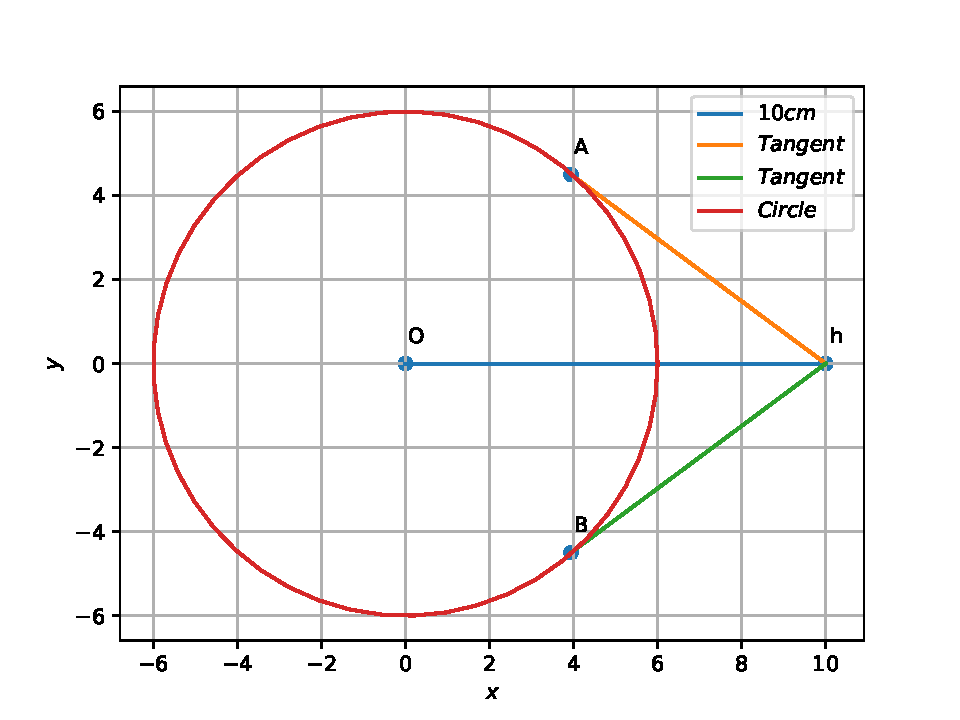
\includegraphics[width=\columnwidth]{chapters/10/11/2/1/figs/circle1.pdf}
		\caption{}
		\label{fig:10/11/2/1}
  	\end{figure}
	\\
	\solution  Follow the approach in Problem  
\ref{chapters/10/10/2/6}.
\iffalse
}

\section*{\large Solution}

\section*{\large Construction}

\begin{figure}[h]
\centering
\includegraphics[width=1\columnwidth]{circle1.pdf}
\caption{Figure}
\label{fig:triangle}
\end{figure}

The dimensions of the figure is taken as below\\\\
{
\setlength\extrarowheight{2pt}
\centering
\begin{tabular}{|c|c|c|}
 \hline
 \textbf{Symbol}&\textbf{Value}&\textbf{Description}\\
 \hline
 r&6&Radius\\
 \hline
 h&10&distance\\
 \hline
 0&$d%
 \begin{pmatrix}
  cos(0)\\
  sin(0)\\
 \end{pmatrix}$%
 &centre\\
 \hline
 A&$a%
 \begin{pmatrix}
  cos\theta\\
  sin\theta\\
 \end{pmatrix}$%
 &point of contact\\
 \hline
 B&$b%
 \begin{pmatrix}
  cos\theta\\
  sin\theta\\
 \end{pmatrix}$%
 &point of contact\\
 \hline
\end{tabular}
}	
\\\\
	The equation of a conic with directrix $\vec{n^Tx}$ = c , eccentricity e anf focus $\boldsymbol{f}$ is given by
	
\begin{equation}
	\vec{x}^T\vec{V}\vec{x} + 2\vec{u}^T + f = 0
\end{equation}
	for circle eccentricity e = 0 then,\\
\begin{equation}
	\vec{V} = \vec{I} = \myvec{1&0\\0&1} , \vec{u} = \myvec{0\\0} , f = -r^2
\end{equation}
Point q on conic is given by 
\begin{equation}
	\vec{q} = \vec{V}^{-1}(\vec{n} - \vec{u})
\end{equation}
where, $\vec{n}$ is the normal vectors of the tangents from a point h to the conic are given by 
\begin{equation}
	\vec{n} = \frac{\vec{e_1}}{\vec{e_1^Th}} + \mu_i(\vec{Rh})
\end{equation}
\\
where $\mu _i$ 's are given by the following equation
\begin{equation}
	\mu_i = \frac{1}{\vec{{m^TVm}}}(\vec{-m^T(Vq+u)})	
\end{equation}
	 			$ \pm \sqrt{\vec{m^T(Vq+u)}^2 - (\vec{q^TVq + 2u^T} + f)(\vec{m^TVm)})}$
\\\\
$\mu _i$ 's are obtained by substituting the following in equation 6\\\\
\begin{equation}
	\vec{m} = (\vec{Rh})  ;  \vec{u}  = \myvec{0\\0}  ;  \vec{q} = \frac{\vec{e_1}}{\vec{e_1^Th}}
\end{equation}
 $\vec{R}$ = $\myvec{0&-1\\1&0}$ 
The obtained $\mu_i$'s are substituted in equation 5 and equation 5 is substituted in equation 6 the required points on conic A and B are obtained.\\\\
Now the point A and B are formed and tangents are drawn \\\\
To find the length of point h and point A \\
\begin{center}
	The distance between h and A is $\norm{\vec{h}-\vec{A}}$\\
\end{center}
\begin{equation}
  (\vec{h}-\vec{A})(\vec{h}-\vec{A})^T=d^2
\end{equation}
\begin{center}
	By solving  equation(7) we get \\
	    distance  d=$8cm$\\
	    \begin{equation}
  (\vec{h}-\vec{A})(\vec{h}-\vec{A})^T=d^2
\end{equation}
\end{center}
\begin{center}
	By solving  equation(7) we get \\
	    distance  d=$8cm$\\
	    \begin{equation}
	    \norm{\vec{h}-\vec{A}}=8cm
	    \end{equation}=8cm
\end{center}
To find the length of point h and point B\\
\begin{center}
	The distance between h and B is $\norm{\vec{h}-\vec{B}}$\\
\end{center}
\begin{equation}
  (\vec{h}-\vec{B})(\vec{h}-\vec{B})^T=d^2
\end{equation}
\begin{center}
	By solving  equation(10) we get \\
	    distance  d=$8cm$\\
	    \begin{equation}
	    \norm{\vec{h}-\vec{B}}=8cm
	    \end{equation}
	    from equation (9) and (11)\\
	    \begin{equation}
	    \norm{\vec{h}-\vec{A}}=\norm{\vec{h}-\vec{B}}
	    \end{equation}
	    \end{center}
	    Hence,the above equation (12) we can prove that the lenght of the tangents to a circle of radius 6cm,from a point 10cm away from the centre of the circle,is 8cm.\\
	    
	    
The below python code realizes the above construction:	\\
\begin{lstlisting}
https://github.com/soundaryanaru/FWC-assignments/blob/main/Matrix/circle_assignment/code/circle.py
\end{lstlisting}
\bibliographystyle{ieeetr}
\end{document}
\fi

\item 
\label{chapters/10/11/2/2}
\iffalse
\documentclass[a4paper,10pt]{report}
\usepackage[latin1]{inputenc}
\usepackage{amsmath}
\usepackage{amsmath,bm}
\usepackage{amsthm}
\usepackage{mathtools}
\usepackage{amsfonts}
\usepackage{amssymb}
\usepackage{graphicx}
\usepackage{array}
\usepackage{booktabs}
\usepackage{hyperref}
\usepackage{multicol}
\usepackage[margin=0.5in]{geometry}
\usepackage{karnaugh-map}
\usepackage[framemethod=tikz]{mdframed}
\newcommand{\myvec}[1]{\ensuremath{\begin{pmatrix}#1\end{pmatrix}}}
\let\vec\mathbf
\newcommand{\mydet}[1]{\ensuremath{\begin{vmatrix}#1\end{vmatrix}}}
\providecommand{\mbf}{\mathbf}
\providecommand{\pr}[1]{\ensuremath{\Pr\left(#1\right)}}
\providecommand{\qfunc}[1]{\ensuremath{Q\left(#1\right)}}
\providecommand{\sbrak}[1]{\ensuremath{{}\left[#1\right]}}
\providecommand{\lsbrak}[1]{\ensuremath{{}\left[#1\right.}}
\providecommand{\rsbrak}[1]{\ensuremath{{}\left.#1\right]}}
\providecommand{\brak}[1]{\ensuremath{\left(#1\right)}}
\providecommand{\lbrak}[1]{\ensuremath{\left(#1\right.}}
\providecommand{\rbrak}[1]{\ensuremath{\left.#1\right)}}
\providecommand{\cbrak}[1]{\ensuremath{\left\{#1\right\}}}
\providecommand{\lcbrak}[1]{\ensuremath{\left\{#1\right.}}
\providecommand{\rcbrak}[1]{\ensuremath{\left.#1\right\}}}
\begin{document}
\raggedright{
\includegraphics[scale=0.07]{logo.jpg}}\hspace{12.425cm}\raggedleft FWC22025\vspace{2mm}\\
\centering\Large\textbf{MATRICES-CIRCLES}\vspace{5mm}
\begin{multicols}{2}
\centering \large\textsc{C}\footnotesize\textsc{ONTENTS}\vspace{5mm}\\
\raggedright\large\textbf{1\hspace{1cm}Problem}\hspace{5.2cm}1\vspace{5mm}\\
\raggedright\large\textbf{2\hspace{1cm}Solution}\hspace{5.25cm}1\vspace{5mm}\\
\raggedright\large\textbf{3\hspace{1cm}Construction}\hspace{4.25cm}2\vspace{5mm}\\
\centering \large\textsc{1  P}\footnotesize\textsc{ROBLEM}\vspace{5mm}\\
\raggedright\large{
\fi
	Construct a tangent to a circle of radius 4cm from a point on the concentric circle of radius 6cm and measure its length. Also verify the measurement by actual calculation.
	\\
	\solution See Fig. 
		\ref{fig:10/11/2/2}.
	\begin{figure}[!ht]
		\centering
 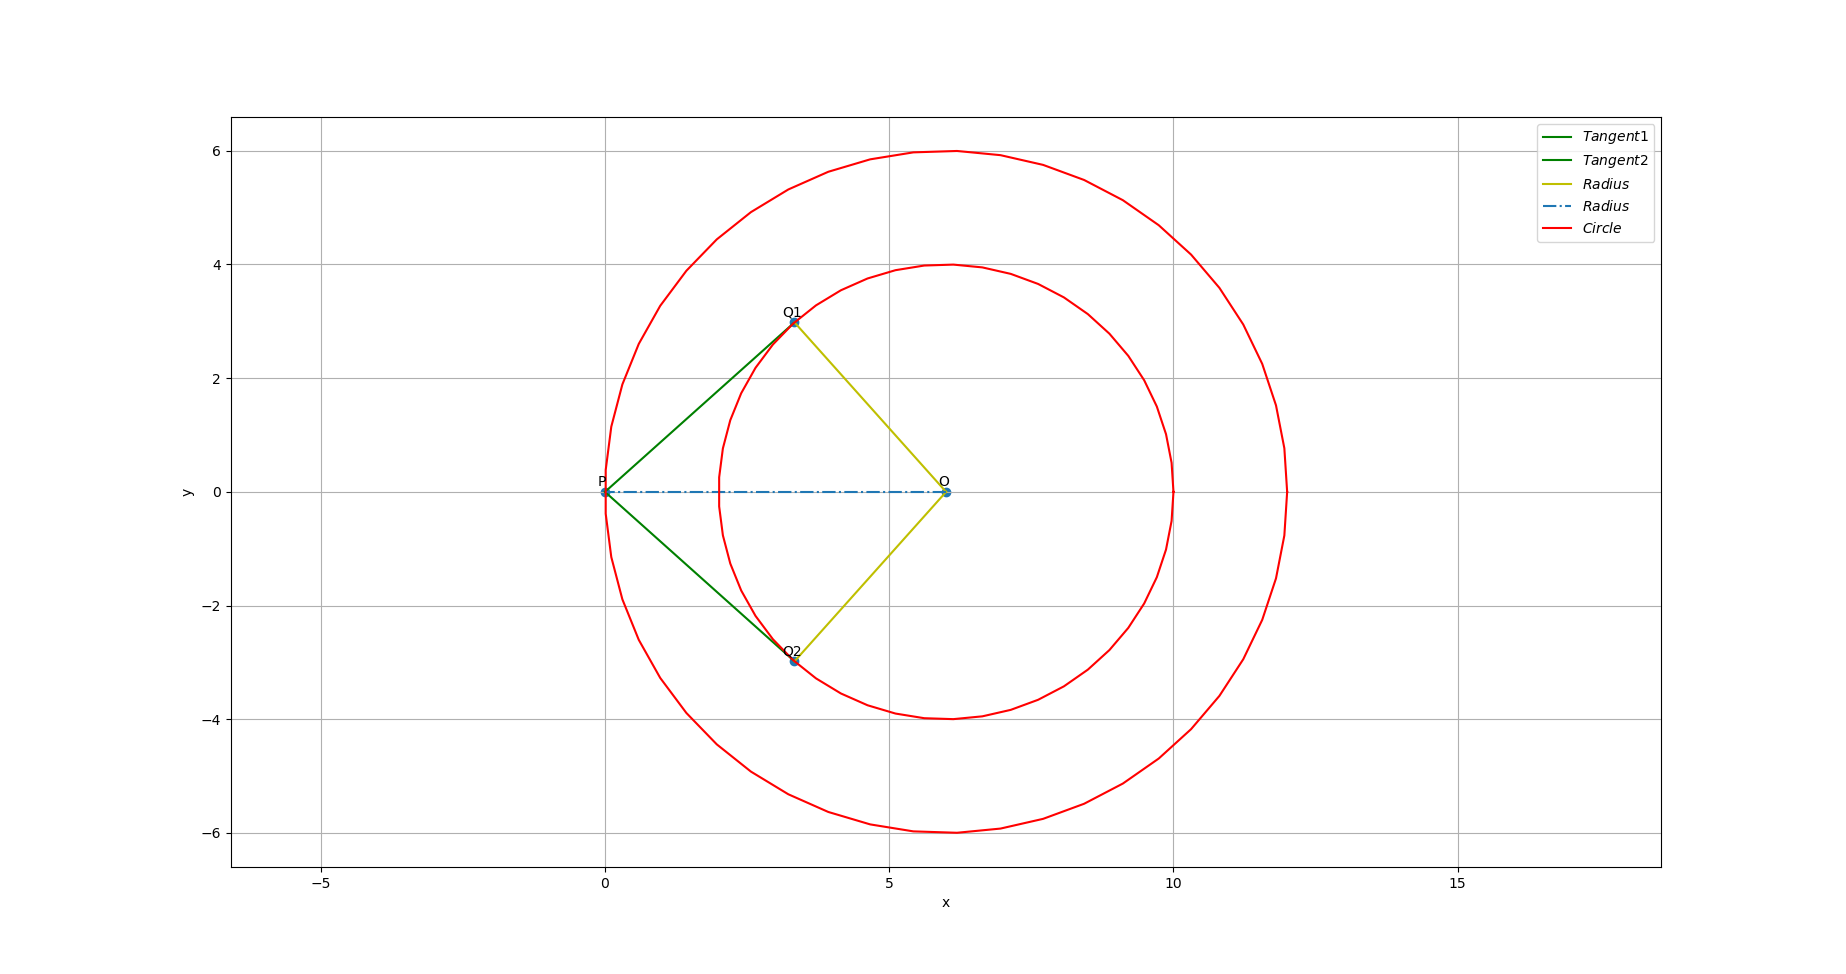
\includegraphics[width=\columnwidth]{chapters/10/11/2/2/figs/main.png}
		\caption{}
		\label{fig:10/11/2/2}
  	\end{figure}
\iffalse
	}\vspace{5mm}\\
\centering \large\textsc{2  S}\footnotesize\textsc{OLUTION}\vspace{5mm}\\
\raggedright\large{Consider a point P on the circle of radius 6 cm is at the origin and the center of circle is at d distance from P (where d=6).}\vspace{2mm}\\
\raggedright\large{Two tangents can be drawn from point P on to the circle of radius 4 cm which is concentric to the circle of radius 6 cm and let the point of contacts be Q1 and Q2.}\vspace{2mm}\\
\raggedright\large{The point of intersection of line \begin{align}L: \quad \vec{x} = \vec{q} + \mu \vec{m} \quad \mu \in \mathbb{R}\end{align} with the conic section \begin{align}\vec{x}^{\top}\vec{V}\vec{x}+2\vec{u}^{\top}\vec{x}+f=0\end{align} is given by \begin{align}\vec{x}_i = \vec{q} + \mu_i \vec{m}\end{align}}
where
\begin{multline}
\mu_i = \frac{1}
{
\vec{m}^{\top}\vec{V}\vec{m}
}
\lbrak{-\vec{m}^{\top}\brak{\vec{V}\vec{q}+\vec{u}}}
\\
\pm
{\small
\rbrak{\sqrt{
\sbrak{
\vec{m}^{\top}\brak{\vec{V}\vec{q}+\vec{u}}
}^2
-
\brak
{
\vec{q}^{\top}\vec{V}\vec{q} + 2\vec{u}^{\top}\vec{q} +f
}
\brak{\vec{m}^{\top}\vec{V}\vec{m}}
}
}
}
\end{multline}
\raggedright\large{If the line L touches the conic at exactly one point $\vec{q}$,}
\begin{align}
\vec{m}^{\top}\brak{\vec{V}\vec{q}+\vec{u}} = 0
\end{align}
\raggedright{In this case, the conic intercept has exactly one root.Hence,}
\begin{align}
  \sbrak{
  \vec{m}^{\top}\brak{\vec{V}\vec{q}+\vec{u}}
  }^2 -\brak{\vec{m}^{\top}\vec{V}\vec{m}}
  \brak
  {
  \vec{q}^{\top}\vec{V}\vec{q} + 2\vec{u}^{\top}\vec{q} +f
  } = 0                                                                                             
\end{align}\vspace{0.5cm}\\
\raggedright\large{So, the equation of conic  $(x-6)^2 + y^2 = 16$ can be written in the form of eq (2) as,}
\begin{align}
\vec{x}^{\top}\myvec{1&0\\0&1}\vec{x}+2\myvec{-6&0}\vec{x}+f=0
\end{align}
\raggedright\large{Let us conisder the direction vector m as,}
\begin{align}
\vec{m}=\myvec{1\\ \lambda}
\end{align}
\raggedright\large{and $\vec{q}$ be the point P,}
\begin{align}
\vec{q}=\myvec{0\\0}
\end{align}
\raggedright\large{Substituting (7),(8) and (9) in eq (6), we get}
\begin{align*}\vspace{0.5cm}\\
\sbrak{\vec{m}^{\top}\brak{\vec{u}}}^2 - f\brak{\vec{m}^{\top}\vec{V}\vec{m}}=0
\end{align*}
\begin{gather*}
\sbrak{\myvec{1& \lambda}\myvec{-6\\0}}^2 - 20\myvec{1 & \lambda}\myvec{1&0\\0&1}\myvec{1\\ \lambda}=0\\
36 - 20\brak{\myvec{1& \lambda}\myvec{1\\ \lambda}}=0\\
36 - 20\brak{1+\lambda^2}=0\\
16 = 20\lambda^2\\
\lambda = \pm 2/\sqrt{5}
\end{gather*}\vspace{0.5cm}\\
\raggedright{Let m1 and m2 be direction vectors of two tangents PQ1 and PQ2, then}
\begin{align*}
\vec{m1}=\myvec{1\\ \frac{2}{\sqrt{5}}}\\
\vec{m2}=\myvec{1\\ \frac{-2}{\sqrt{5}}}
\end{align*}\vspace{0.5cm}\\
\raggedright\large{Substituting (6) in (4), we get}
\begin{align}
\mu_i = \frac{1}
{
\vec{m}^{\top}\vec{V}\vec{m}
}
\lbrak{-\vec{m}^{\top}\brak{\vec{V}\vec{q}+\vec{u}}}
\end{align}
\raggedright\large{Substituting m1 and m2 in (10),we get}\\
\begin{gather*}
\mu_1 = \frac{10}{3} \hspace{0.1cm}and\hspace{0.1cm} \mu_2 = \frac{10}{3}
\end{gather*}
\raggedright\large{Hence,}
\begin{align}
\vec{x}_1 = \vec{q} + \mu_1 \vec{m1}\vspace{2mm}\\
\vec{x}_2 = \vec{q} + \mu_2 \vec{m2}
\end{align}
\raggedright\large{Solving above equations, we get}
\begin{align*}
\vec{x}_1 = \myvec{\frac{10}{3}\vspace{2mm}\\\frac{20}{3\sqrt{5}}}
\implies{\vec{x}_1 = \myvec{3.33 \\ 2.98}}\\
\vec{x}_2 = \myvec{\frac{10}{3}\vspace{2mm}\\\frac{-20}{3\sqrt{5}}}
\implies{\vec{x}_2 = \myvec{3.33 \\ -2.98}}
\end{align*}
\raggedright\large{Thus,}
\begin{align}
\vec{Q1} = \vec{x}_1\hspace{0.1cm} and \hspace{0.1cm}\vec{Q2} = \vec{x}_2
\end{align}\vspace{5mm}\\

\centering{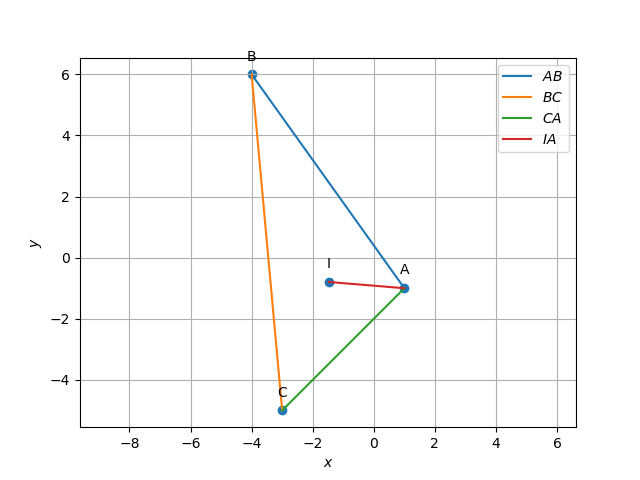
\includegraphics[scale=0.2]{main.png}}\vspace{2mm}\\
\centering{Figure}\vspace{2mm}\\
\centering \large\textsc{3  C}\footnotesize\textsc{ONSTRUCTION}\vspace{5mm}\\
\raggedright\large{The concentric circles and tangents are constructed with,} 
\begin{center}
    \label{tab:truthtable}
    \setlength{\arrayrulewidth}{0.2mm}
\setlength{\tabcolsep}{5pt}
\renewcommand{\arraystretch}{1.25}
    \begin{tabular}{|c|c|c|}
    \hline % <-- Alignments: 1st column left, 2nd middle and 3rd right, with vertical lines in between
      \large\textbf{Symbol} & \large\textbf{Co-ordinates} & \large\textbf{Description}\\
      \hline
       \large r1& 4& \large{radius}\\
       \large r2& 6& \large{radius}\\
       \large d & 6 & OP\\
	\large m1 & $\ \begin{pmatrix} 1\\\frac{2}{\sqrt{5}} \end{pmatrix}$ & \large direction vector of PQ1\\
	\large m2 & $\ \begin{pmatrix} 1\\\frac{-2}{\sqrt{5}} \end{pmatrix}$ & \large direction vector of PQ2\\
        \large$ \mu_1$ & $\frac{10}{3}$ & \large{root}\\
	\large $\mu_2$ & $\frac{10}{3}$ & \large{root}\\
        \large P & $\ \begin{pmatrix} 0\\0 \end{pmatrix}$ & \large point vector P\\
	\large O & $\ \begin{pmatrix} d\\0 \end{pmatrix}$ & \large point vector O\\
	\large \textbf{Q1} & $\mu_1\vec{m1}$ & point of contact 1\\
	\large \textbf{Q2} & $\mu_2\vec{m2}$ & point of contact 2\\
      \hline
   \end{tabular}
 \end{center}\vspace{5mm}
\raggedright\large{The figure above is generated using python code provided in the below source code link.}\vspace{2mm}\\
\begin{mdframed}
\raggedright\large{https://github.com/madind5668 \\ /FWC/blob/main/matrices/circles \\ /codes/main.py}
\end{mdframed}
\end{multicols}
\end{document}
\fi


\item 
\label{chapters/10/11/2/3}
\\
\solution See Fig. 
		\ref{fig:10/11/2/3}.
	\begin{figure}[!ht]
		\centering
 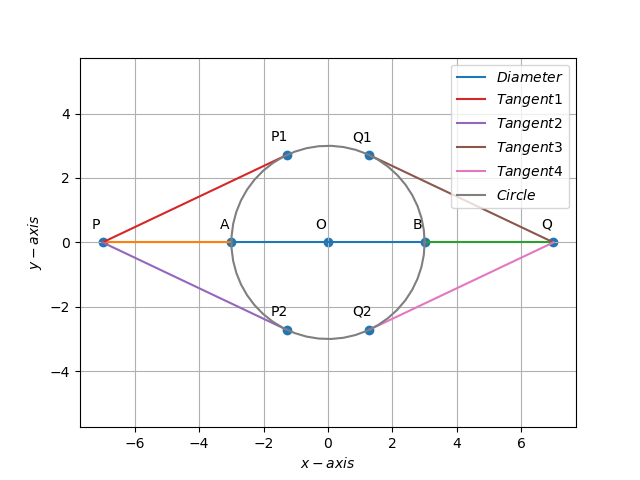
\includegraphics[width=\columnwidth]{chapters/10/11/2/3/figs/Question.png}
		\caption{}
		\label{fig:10/11/2/3}
  	\end{figure}

\item 
\label{chapters/10/11/2/4}
\iffalse
\documentclass{article}
% Language setting
% Replace `english' with e.g. `spanish' to change the document language
\usepackage[english]{babel}
% Set page size and margins
% Replace `letterpaper' with `a4paper' for UK/EU standard size
\usepackage[letterpaper,top=2cm,bottom=2cm,left=3cm,right=3cm,marginparwidth=1.75cm]{geometry}
% Useful packages
\usepackage{multicol}
\usepackage{amsmath}
\usepackage{amssymb}
\usepackage{graphicx}
\usepackage[framemethod=tikz]{mdframed}
\usepackage{array}
\usepackage{blindtext}
%\usepackage[paperwidth=10cm]{geometry}
\usepackage{tkz-euclide}
%\usepackage{tikz}
\usetikzlibrary{
  circuits.logic,
  circuits.logic.US,
  positioning
}

\usepackage[colorlinks=true, allcolors=blue]{hyperref}
\newcommand{\myvec}[1]{\ensuremath{\begin{pmatrix}#1\end{pmatrix}}}
\providecommand{\norm}[1]{\left\lVert#1\right\rVert}
\let\vec\mathbf
\title{Circle Assignment}
\author{Anusha Jella}
\begin{document}
\maketitle
\newtheorem{theorem}{Theorem}[section]
\begin{multicols}{2}

\paragraph{\begin{flushleft}\textbf{Problem: }
\textbf
	\fi
	Draw a pair of tangents to a circle of radius 5 cm which are inclined to each other at an angle of 60\degree.
	\\
	\solution See Fig. 
		\ref{fig:10/11/2/4}.
	\begin{figure}[!ht]
		\centering
 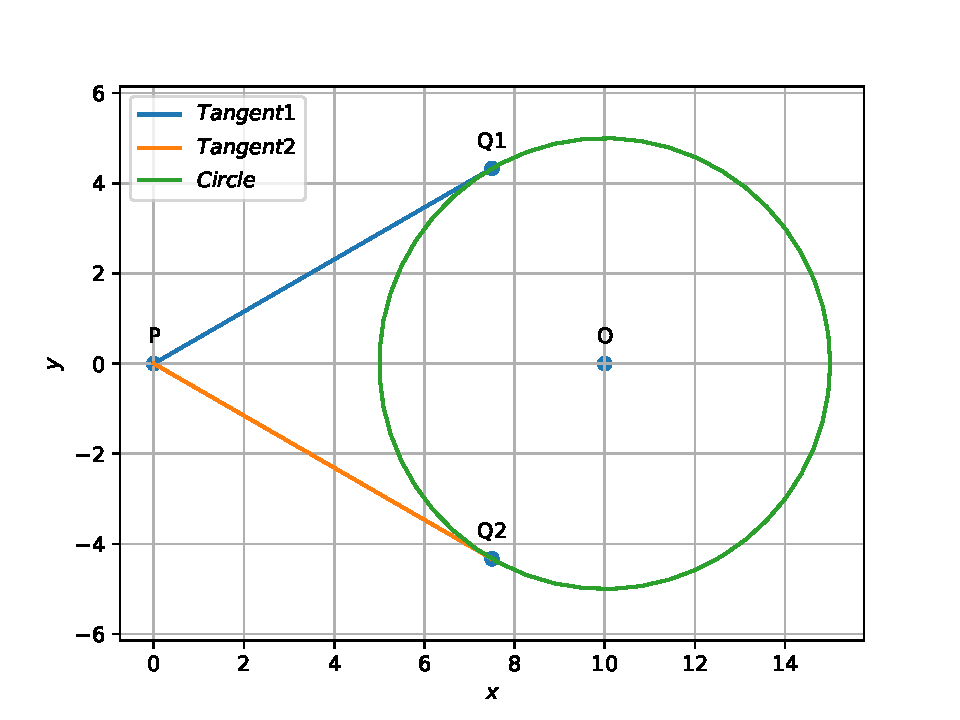
\includegraphics[width=\columnwidth]{chapters/10/11/2/4/figs/circle1.pdf}
		\caption{}
		\label{fig:10/11/2/4}
  	\end{figure}
\iffalse
	$^{\circ}$.}
\end{flushleft}}
%\begin{figure}[h]
\centering
\includegraphics[scale=0.5]{circle_fig2.pdf}  
%\includegraphics[width=\columnwidth]{circle1.pdf} 
\centering{Fig 1. Circle}
\label{fig:circle_1}
%\end{figure}

 \section*{Construction}
 \begin{flushleft}
 \textsc{solution:} The following python code is used for constructing circle with pair of tangents.
 \end{flushleft}
 \begin{mdframed}
   \url{https://github.com/AnushaJella/assignment_circle/blob/main/circle1.py}\\
\end{mdframed}
See Fig 1 for the input parameters in Table 1.\\
{\setlength\extrarowheight{2pt}
\begin{tabular}{|c|c|c|}
	\hline
	\textbf{Symbol}&\textbf{Value}&\textbf{Description}\\
	\hline
	O&$\begin{pmatrix}
	0\\0\\
	\end{pmatrix} $&Center $\vec{O}$\\
	\hline
	$\theta_{1}$&60$^{\circ}$& $\angle$$Q_1$P$Q_2$\\
	\hline
	r&5& radius of circle\\
	\hline
	
\end{tabular}
}\\
\centering {Table 1}\\
\hspace{-6cm}In $\Delta$Oqh 
\begin{align}
	\boldsymbol{h} = r\csc\frac{\theta}{2} e1
\end{align}
\section*{Solution}
\begin{flushleft}
The equation of  a conic with directrix $\vec{n}^{\top}\vec{x} = c$, eccentricity $e$ and focus $\vec{F}$ is given by 
\end{flushleft}
\begin{align}
    \vec{x}^{\top}\vec{V}\vec{x}+2\vec{u}^{\top}\vec{x}+f=0
\end{align}
\hspace{-2cm}for circle eccentricity e=0
then, 
\begin{align}
	\vec{V}
	=\vec{I},
\vec{u} = \myvec{0\\0},  f = -r^2.
	\label{eq:matrix-10-13-param}
\end{align}
\hspace{-2.5cm}Point q on conic is given by
\begin{align*}
q=\vec{V}^{-1}(k_i\vec{n}-\vec{u}^T)^T \\
\hspace{-6cm}where,\\
k_i=\pm \sqrt{\frac{f_0}{\vec{n}^T\vec{V}^{-1}\vec{n}}}\\
f_0=f+\vec{u}^T\vec{V}^{-1}\vec{u}\\
n=P\myvec{\sqrt{\lambda_1}\\\pm \sqrt{\lambda_2}}
\end{align*}
\hspace{-2cm}$\vec{P}$,$\lambda_{1,2}$ are eigen parameters of 
\begin{align*}
\sum=(\vec{V}\vec{h}+\vec{u})(\vec{V}\vec{h}+\vec{u})^T-\vec{V}(\vec{h}^T\vec{V}\vec{h}+2\vec{u}^Th+f)
\end{align*}
\end{multicols}{2}
\end{document}
\fi

\item 
\label{chapters/10/11/2/5}
\iffalse
\documentclass[journal,12pt,twocolumn]{IEEEtran}

\usepackage[utf8]{inputenc}
\usepackage{kvmap}
\usepackage{graphics} 

\usepackage{setspace}
\usepackage{gensymb}

\singlespacing


\usepackage{amsthm}

\usepackage{mathrsfs}
\usepackage{txfonts}
\usepackage{stfloats}
\usepackage{bm}
\usepackage{cite}
\usepackage{cases}
\usepackage{subfig}

\usepackage{longtable}
\usepackage{multirow}

\usepackage{enumitem}
\usepackage{mathtools}
\usepackage{steinmetz}
\usepackage{tikz}
\usepackage{circuitikz}
\usepackage{verbatim}
\usepackage{tfrupee}
\usepackage[breaklinks=true]{hyperref}
\usepackage{graphicx}
\usepackage{tkz-euclide}
\usepackage{float}

\usetikzlibrary{calc,math}
\usepackage{listings}
    \usepackage{color}                                            %%
    \usepackage{array}                                            %%
    \usepackage{longtable}                                        %%
    \usepackage{calc}                                             %%
    \usepackage{multirow}                                         %%
    \usepackage{hhline}                                           %%
    \usepackage{ifthen}                                           %%
    \usepackage{lscape}     
\usepackage{multicol}
\usepackage{chngcntr}

\DeclareMathOperator*{\Res}{Res}

\renewcommand\thesection{\arabic{section}}
\renewcommand\thesubsection{\thesection.\arabic{subsection}}
\renewcommand\thesubsubsection{\thesubsection.\arabic{subsubsection}}

\renewcommand\thesectiondis{\arabic{section}}
\renewcommand\thesubsectiondis{\thesectiondis.\arabic{subsection}}
\renewcommand\thesubsubsectiondis{\thesubsectiondis.\arabic{subsubsection}}


\hyphenation{op-tical net-works semi-conduc-tor}
\def\inputGnumericTable{}                                 %%

\lstset{
%language=C,
frame=single, 
breaklines=true,
columns=fullflexible
}
\begin{document}


\newtheorem{theorem}{Theorem}[section]
\newtheorem{problem}{Problem}
\newtheorem{proposition}{Proposition}[section]
\newtheorem{lemma}{Lemma}[section]
\newtheorem{corollary}[theorem]{Corollary}
\newtheorem{example}{Example}[section]
\newtheorem{definition}[problem]{Definition}

\newcommand{\BEQA}{\begin{eqnarray}}
\newcommand{\EEQA}{\end{eqnarray}}
\newcommand{\define}{\stackrel{\triangle}{=}}
\newcommand\hlight[1]{\tikz[overlay, remember picture,baseline=-\the\dimexpr\fontdimen22\textfont2\relax]\node[rectangle,fill=blue!50,rounded corners,fill opacity = 0.2,draw,thick,text opacity =1] {$#1$};}
\bibliographystyle{IEEEtran}
\providecommand{\mbf}{\mathbf}
\providecommand{\pr}[1]{\ensuremath{\Pr\left(#1\right)}}
\providecommand{\qfunc}[1]{\ensuremath{Q\left(#1\right)}}
\providecommand{\sbrak}[1]{\ensuremath{{}\left[#1\right]}}
\providecommand{\lsbrak}[1]{\ensuremath{{}\left[#1\right.}}
\providecommand{\rsbrak}[1]{\ensuremath{{}\left.#1\right]}}
\providecommand{\brak}[1]{\ensuremath{\left(#1\right)}}
\providecommand{\lbrak}[1]{\ensuremath{\left(#1\right.}}
\providecommand{\rbrak}[1]{\ensuremath{\left.#1\right)}}
\providecommand{\cbrak}[1]{\ensuremath{\left\{#1\right\}}}
\providecommand{\lcbrak}[1]{\ensuremath{\left\{#1\right.}}
\providecommand{\rcbrak}[1]{\ensuremath{\left.#1\right\}}}
\theoremstyle{remark}
\newtheorem{rem}{Remark}
\newcommand{\sgn}{\mathop{\mathrm{sgn}}}
\providecommand{\abs}[1]{\left\vert#1\right\vert}
\providecommand{\res}[1]{\Res\displaylimits_{#1}} 
\providecommand{\norm}[1]{$\left\lVert#1\right\rVert$}
%\providecommand{\norm}[1]{\lVert#1\rVert}
\providecommand{\mtx}[1]{\mathbf{#1}}
\providecommand{\mean}[1]{E\left[ #1 \right]}
\providecommand{\fourier}{\overset{\mathcal{F}}{ \rightleftharpoons}}
%\providecommand{\hilbert}{\overset{\mathcal{H}}{ \rightleftharpoons}}
\providecommand{\system}{\overset{\mathcal{H}}{ \longleftrightarrow}}
	%\newcommand{\solution}[2]{\textbf{Solution:}{#1}}
\newcommand{\solution}{\noindent \textbf{Solution: }}
\newcommand{\cosec}{\,\text{cosec}\,}
\providecommand{\dec}[2]{\ensuremath{\overset{#1}{\underset{#2}{\gtrless}}}}
\newcommand{\myvec}[1]{\ensuremath{\begin{pmatrix}#1\end{pmatrix}}}
\newcommand{\mydet}[1]{\ensuremath{\begin{vmatrix}#1\end{vmatrix}}}
\numberwithin{equation}{subsection}
\makeatletter
\@addtoreset{figure}{problem}
\makeatother
\let\StandardTheFigure\thefigure
\let\vec\mathbf
\renewcommand{\thefigure}{\theproblem}
\def\putbox#1#2#3{\makebox[0in][l]{\makebox[#1][l]{}\raisebox{\baselineskip}[0in][0in]{\raisebox{#2}[0in][0in]{#3}}}}
     \def\rightbox#1{\makebox[0in][r]{#1}}
     \def\centbox#1{\makebox[0in]{#1}}
     \def\topbox#1{\raisebox{-\baselineskip}[0in][0in]{#1}}
     \def\midbox#1{\raisebox{-0.5\baselineskip}[0in][0in]{#1}}
\vspace{3cm}
\title{\textbf{Matrix Assignment - Circle} }
\author{Surabhi Seetha}
\maketitle
\newpage
\bigskip
\renewcommand{\thefigure}{\theenumi}
\renewcommand{\thetable}{\theenumi}
Get Python code for the figure from 
\begin{lstlisting}
https://github.com/SurabhiSeetha/Fwciith2022/tree/main/Assignment%201/codes/src
\end{lstlisting}
Get LaTex code from
\begin{lstlisting}
https://github.com/SurabhiSeetha/Fwciith2022/tree/main/avr%20gcc
\end{lstlisting}
%
\section{Question-Class 10, Exercise 11.2, Q(5)}
\textbf{
\fi
	Draw a line segment $AB$ of length 8cm. Taking $\vec{A}$ as centre, draw a circle of radius 4cm and taking $\vec{B}$ as centre, draw another circle of radius 3cm. Construct tangents to each circle from the centre of the circle.
	\\
	\solution See Fig. 
		\ref{fig:10/11/2/5}.
	\begin{figure}[!h]
		\centering
 \includegraphics[width=\columnwidth]{chapters/10/11/2/5/figs/cir.png}
		\caption{}
		\label{fig:10/11/2/5}
  	\end{figure}
	\iffalse
} \\


\centering
\includegraphics[width=0.45\textwidth]{cir.png}
Figure- Circles A and B with tangents P1,P2,Q1,Q2

\section{Construction}
\vspace{0.25cm}
\raggedright
A circle with radius 4cm and another circle with radius 3cm are taken and their tangents are drawn with their point of contacts as P1,P2,Q1 and Q2 and their construction is done with the help of $\theta$ and $\alpha$ angles as shown in the table below.\\
\centering
\begin{tabular}{|c|c|c|}
\hline
\textbf{Symbol} & \textbf{Value} & \textbf{Description} \\
\hline
$r_1$ & 4cm & radius\\
\hline
$r_2$ & 3cm & radius\\
\hline
O & $\myvec{0\\0}$ & Center O\\
\hline
d & 8cm & Distance OC\\
\hline
$e_1$ & $\myvec{1\\0}$ &  Unit Vector\\
\hline
C & d x $e_1$ & Centre C\\
\hline
$\theta$ & $\angle P_1OC$ & Angle $P_1OC$\\
\hline
$\alpha$ & $\angle Q_1OC$ & Angle $Q_1OC$\\
\hline
t & d $cos\alpha$ & $OQ_1$ \\
\hline
$P_1$ & $r_1$ $\myvec{cos\theta\\ sin\theta}$ & P.O.C \\
\hline
$P_2$ & $r_1$ $\myvec{cos\theta\\ -sin\theta}$ & P.O.C \\
\hline
$Q_1$ & t $\myvec{cos\alpha\\ sin\alpha}$ & P.O.C \\
\hline
$Q_2$ & t $\myvec{cos\alpha\\ -sin\alpha}$ & P.O.C \\
\hline

\end{tabular}

\section{Solution}
\raggedright{\subsection{Part-1:}}
Consider the circle A of radius 4cm and points O and C each at a distance 8cm from the centre. Two tangents can be drawn from point O onto the circle B with point of contacts Q1,Q2 and other two tangents from point C onto the circle A with the point of contacts P1,P2.\\
\vspace{0.25cm}
\raggedright{The point of intersection of line:}\\
\begin{align}
L:\textbf{x}=\textbf{q}+\mu \textbf{m}           
\label{eq1}
\end{align}
\raggedright{with the conic section:}\\
\begin{align}
\textbf{x}^T\textbf{Vx}+2\textbf{u}^T\textbf{x}+f=0     
\label{eq2}
\end{align}
\raggedright{is given by-}\\
\begin{align}
\vec{x_i}=\vec{q}+\mu_i\vec{m}             
\label{eq3}
\end{align}
\raggedright{where,}\\
$\mu_i=\frac{1}{\vec{m}^T\vec{Vm}}(-\vec{m}^T(\vec{Vq}+\vec{u})$\\ 
\begin{align}
\pm\sqrt{(\vec{m}^T(\vec{Vq+u}))^2-(\vec{q}^T+2\vec{u}^T\vec{q}+f)(\vec{m}^T\vec{Vm})}                 
\label{eq4}
\end{align}
\vspace{0.25cm}
\raggedright{If the line L touches the conic at exactly one point q}\\
where q is the point of origin(0,0) which is A\\
\begin{align}
\vec{m}^T(\vec{Vq}+\vec{u}=0)                 
\label{eq5}
\end{align}

\vspace{0.25cm}
\raggedright
In this case,the conic intercept has exactly one root Hence,\\
\vspace{0.25cm}
\begin{align}
[\vec{m}^T(\vec{Vq}+\vec{u})]^2-(\vec{m}^T\vec{Vm})(\vec{q}^T\vec{Vq}+2\vec{u}^T\vec{q}+f)=0    
\label{eq6}
\end{align}
\raggedright\vspace{0.25cm}
So,comparing the equation of our conic $x^2+y^2=4^2$ with the general Equation of a circle:\\
\vspace{0.25cm}
\centering{$Ax^2+Bxy+Cy^2+Fx+Gy+f=0$}\\
\centering\vspace{0.15cm}{$x^2+y^2-16=0$}\\
\raggedright{we get,}\\
\vspace{0.15cm}
\centering{$\vec{V}=\myvec{A&\frac{B}{2} \\\\ \frac{B}{2}&C}$}
\hspace{1.5cm}$\vec{u}=\myvec{\frac{F}{2} \\\\ \frac{G}{2}}$\\
\vspace{0.25cm}
\hspace{0.3cm}{$\vec{V}=\myvec{1&0 \\\\ 0&1}$}
\hspace{1.5cm} $\vec{u}=\myvec{0 \\ 0}$\\
\vspace{0.25cm}
\raggedright
Substituting the above values in eq.\eqref{eq2} we get,\\
\vspace{0.25cm}
\begin{align}
\vec{x}^T\vec{Vx}+2(0\hspace{0.2cm}0)\vec{x}+4=0        
\label{eq7}
\end{align}
\vspace{0.25cm}
\raggedright{Let us consider the direction vector of L as m}\\
\vspace{0.25cm}
\begin{align}
\vec{m}=\myvec{1 \\ \lambda}    
\label{eq8}
\end{align}
\raggedright{and q be the pont A,}\\
\begin{align}
\vec{q}=\myvec{8 \\ 0}        
\label{eq9}
\end{align}
\raggedright{Substituting eq. \eqref{eq7}, \eqref{eq8} and \eqref{eq9} in Eq.\eqref{eq6} we get,}\\
\vspace{0.25cm}
\centering{$[\vec{m}^T(\vec{Iq})]^2-(\vec{m}^T\vec{Im})(\vec{q}^T\vec{Iq}+(-16))=0$}\\
\vspace{0.3cm}
\begin{align}
[\myvec{1&\lambda} \myvec{8 \\ 0}]^2-(\myvec{1&\lambda} \myvec{1 \\ \lambda})(\myvec{8&0}\myvec{8 \\ 0}-16)=0    
\label{eq10}
\end{align}
\vspace{0.25cm}
\centering{$8^2-(1+\lambda^2)(64-16)=0$}\\
\vspace{0.25cm}
$64-(1+\lambda^2)(48)=0$\\
\vspace{0.25cm}
$(1+\lambda^2)=\frac{64}{48}$\\
\vspace{0.25cm}
\begin{align}
\vec{\lambda}=\pm\frac{1}{\sqrt{3}}         
\label{eq11}
\end{align}
\raggedright{That is,}\\
\vspace{0.25cm}
\begin{align}
\vec{m}=\myvec{1  \\ \pm{\frac{1}{\sqrt{3}}}}         
\label{eq12}
\end{align}
\raggedright{from \eqref{eq4} and \eqref{eq6}}\\
\vspace{0.25cm}
\begin{align}
\mu_i=\frac{1}{\vec{m}^T\vec{Vm}}(\vec{-m}^T(\vec{Vq}+\vec{u})) 
\label{eq13}
\end{align}
\vspace{0.25cm}
$ \mu_i = \frac{1}{\myvec{1 \\ \frac{1}{\sqrt{3}}} I \myvec{1 & \frac{1}{\sqrt{3}}}} (-(1 \pm\frac{1}{\sqrt{3}}\myvec{8 \\ 0})$\\
\vspace{0.25cm}
$\mu_i=\frac{1}{1+\frac{1}{3}}(-8)$\\
\vspace{0.25cm}
\begin{align}
\mu_i=-6
\label{eq14}
\end{align}
\vspace{0.25cm}
\raggedright{Now eq. \eqref{eq3} becomes,}\\
\vspace{0.25cm}
\centering
\begin{align}
\myvec{x \\ y} = \myvec{8\\0} + (-6)  \myvec{1 \\ \pm \frac{1}{\sqrt{3}}}
\label{eq15}
\end{align}  
\vspace{0.25cm}
\begin{align}
\myvec{x \\ y} = \myvec{8\\0} + \myvec{-6 \\ \pm \frac{6}{\sqrt{3}}}
\label{eq16}
\end{align}  
\vspace{0.25cm}
\begin{align}
\myvec{x \\ y} = \myvec{2 \\ \pm \frac{6}{\sqrt{3}}}
\label{eq17}
\end{align}  
\vspace{0.25cm}
\raggedright
Therefore,\\
\vspace{0.25cm}
\centering
$ \vec{P_1} = \myvec{2 \\ \frac{6}{\sqrt{3}}} = \myvec{2\\3.464} $\\
\vspace{0.25cm}
$ \vec{P_2} = \myvec{2 \\ -\frac{6}{\sqrt{3}}} = \myvec{2\\-3.464} $\\
\raggedright{\subsection{Part-2:}}
Now for another circle B of radius 3cm which has its tangents drawn from circle A onto B with the point of contacts namely $Q_1$ and $Q_2$.\\
\vspace{0.25cm}
Let us consider the same line and conic equations as in Part 1. The line L touches the conic at exactly one point q.\\
\vspace{0.25cm}
\centering
\begin{align}
\vec{m}^T (\vec{Vq} + \vec{u}) = 0  
\label{eq18}
\end{align}
\vspace{0.25cm}
\raggedright
Hence,\\
\vspace{0.25cm}
\centering
\begin{align}
[ \vec{m}^T (\vec{Vq} + \vec{u}) ]^2 -(\vec{m}^T \vec{Vm})(\vec{q}^T \vec{Vq} + 2\vec{u}^T \vec{q} + f) = 0 
\label{eq19}
\end{align}
\vspace{0.25cm}
\raggedright
The equation of conic is,\\
\vspace{0.25cm}
\centering
$ (x-8)^2 + y^2 = 3^2 $\\
\vspace{0.25cm}
$ x^2 + 64 -16x + y^2 - 9 = 0$ \\
\vspace{0.25cm}
$ x^2 - 16x + y^2 + 55 = 0 $ \\
\vspace{0.25cm}
\raggedright
Comparing it with general Eq. of a circle\\
\vspace{0.25cm}
\centering
$ A x^2 + Bxy + C y^2 + Fx + Gy + f = 0 $\\
\vspace{0.25cm}
\raggedright
We get,\\
\vspace{0.25cm}
\centering{$\vec{V}=\myvec{A&\frac{B}{2} \\\\ \frac{B}{2}&C}$}
\hspace{1.5cm}$\vec{u}=\myvec{\frac{F}{2} \\\\ \frac{G}{2}}$\\
\vspace{0.25cm}
\hspace{0.3cm}{$\vec{V}=\myvec{1&0 \\\\ 0&1}$}
\hspace{1.25cm} $\vec{u}=\myvec{-8 \\\\ 0}$\\
\vspace{0.25cm}
\raggedright
Now Eq. \eqref{eq2} can be written as,\\
\vspace{0.25cm}
\centering
\begin{align}
\vec{x}^T \myvec{1&0\\0&1} x + 2 \myvec{-8&0} \vec{x} + 3 = 0 
\label{eq20}
\end{align}
\vspace{0.25cm}
\raggedright{Let us consider the direction vector of \textbf{L} as m}\\
\vspace{0.25cm}
\begin{align}
\vec{m}=\myvec{1 \\ \lambda}     
\label{eq21}
\end{align}
\raggedright{and q be the pont A,}\\
\begin{align}
\vec{q}=\myvec{0 \\ 0} 
\label{eq22}
\end{align}
\raggedright{Substituting the above values in eq. \eqref{eq19} we get,}\\
\vspace{0.25cm}
\centering
$ [ \vec{m}^T (\vec{Vq} + \vec{u}) ]^2 -(\vec{m}^T \vec{Vm})(\vec{q}^T \vec{Vq} + 2\vec{u}^T \vec{q} + f) = 0$ \\
\vspace{0.25cm}
$ [ \myvec{1 & \lambda} [I \myvec{0\\0} + \myvec{-8 \\ 0}]]^2 - ( \myvec{1&\lambda} I \myvec{1\\ \lambda}) (55) = 0 $ \\
\vspace{0.25cm}
$ [ \myvec{1 & \lambda} \myvec{-8 \\ 0}]^2 - (1 + \lambda^2) (55) = 0 $ \\
\vspace{0.25cm}
$ 64 - ( 1 + \lambda^2 ) 55 = 0 $\\
\vspace{0.25cm}
$ 64 - 55 - 55\lambda^2 = 0 $ \\
\vspace{0.25cm}
$ \lambda^2 = \frac{9}{55}$ \\
\vspace{0.25cm}
\begin{align}
\lambda = \pm \frac{3}{\sqrt{55}} = \pm 0.4
\label{eq23}
\end{align}
\vspace{0.25cm}
\raggedright
Now,\\
\vspace{0.1cm}
\centering
$ \vec{m} = \myvec{1 \\ \pm0.4045} $ \\
\vspace{0.25cm}
\raggedright
From eq. \eqref{eq4} and \eqref{eq6},\\
\vspace{0.25cm}
\centering
$\mu_i=\frac{1}{\vec{m}^T\vec{Vm}}(\vec{-m}^T(\vec{Vq}+\vec{u}))$ \\
\vspace{0.25cm}
$ \mu_i = \frac{1}{\myvec{1\\0.4045} \hspace{0.1cm} I \hspace{0.1cm} \myvec{1 & 0.4045}} (- \myvec{1 & 0.4045} ( I \myvec{0\\0} + \myvec{-8\\0} ) $ \\
\vspace{0.25cm}
\raggedright
\hspace{1cm} $ = \frac{1}{1 + 0.163} ( - \myvec{1 & 0.4045} \myvec{-8 \\ 0} )$ \\
\vspace{0.25cm}
\hspace{1cm} $ = \frac{1}{1.163} \hspace{0.25cm} \times \hspace{0.25cm} 8 $ \\
\vspace{0.25cm}
Therefore,\\
\vspace{0.1cm}
\centering
$ \vec{\mu_i} = \frac{8}{1.163} = 6.875 $ \\
\vspace{0.25cm}
\raggedright
Now eq. \eqref{eq3} becomes,\\
\centering
\vspace{0.1cm}
$ \vec{x_i} = \vec{q} + \mu_i \vec{m} $ \\
\vspace{0.25cm}
$ = \myvec{0\\0} + 6.875 \myvec{1\\ \pm 0.4045} $ \\
\vspace{0.25cm}
\centering
$ x_i = \myvec{x\\y} = \myvec{6.875 \\ \pm 2.7810} $ \\
\vspace{0.25cm}
\raggedright
Therefore,\\
\vspace{0.25cm}
\centering
$ \vec{Q_1} = \myvec{6.875 \\ 2.7810} $ \\
\vspace{0.25cm}
$ \vec{Q_2} = \myvec{6.875 \\ -2.7810} $ \\
\raggedright
\vspace{0.5cm}
Therefore, we have solved and gained the values of four point of contacts P1,P2,Q1,Q2 for two circles of radius 4cm and 3cm.\\
\end{document}
Footer
\fi

\item 
\label{chapters/10/11/2/6}
\iffalse
\documentclass[journal,10pt,twocolumn]{article}
\usepackage{graphicx, float}
\usepackage[margin=0.5in]{geometry}
\usepackage{amsmath, bm}
\usepackage{array}
\usepackage{booktabs}

\providecommand{\norm}[1]{\left\lVert#1\right\rVert}
\let\vec\mathbf
\newcommand{\myvec}[1]{\ensuremath{\begin{pmatrix}#1\end{pmatrix}}}
\newcommand{\mydet}[1]{\ensuremath{\begin{vmatrix}#1\end{vmatrix}}}

\title{\textbf{Circle Assignment}}
\author{Mohamed Hamdan}
\date{September 2022}

\begin{document}

\maketitle
\paragraph{\textit{Problem Statement} -
\fi
Let $ABC$ be a right triangle in which $AB = 6 cm, BC = 8 cm$ and $\angle B = 90\degree$. $BD$ is the perpendicular from $\vec{B}$ on $AC$. The circle through $\vec{B}, \vec{C}, \vec{D}$ is drawn. Construct the tangents from $\vec{A}$ to this circle.
\\
\solution
See Fig. 
		\ref{fig:10/11/2/6}.
	\begin{figure}[!ht]
		\centering
 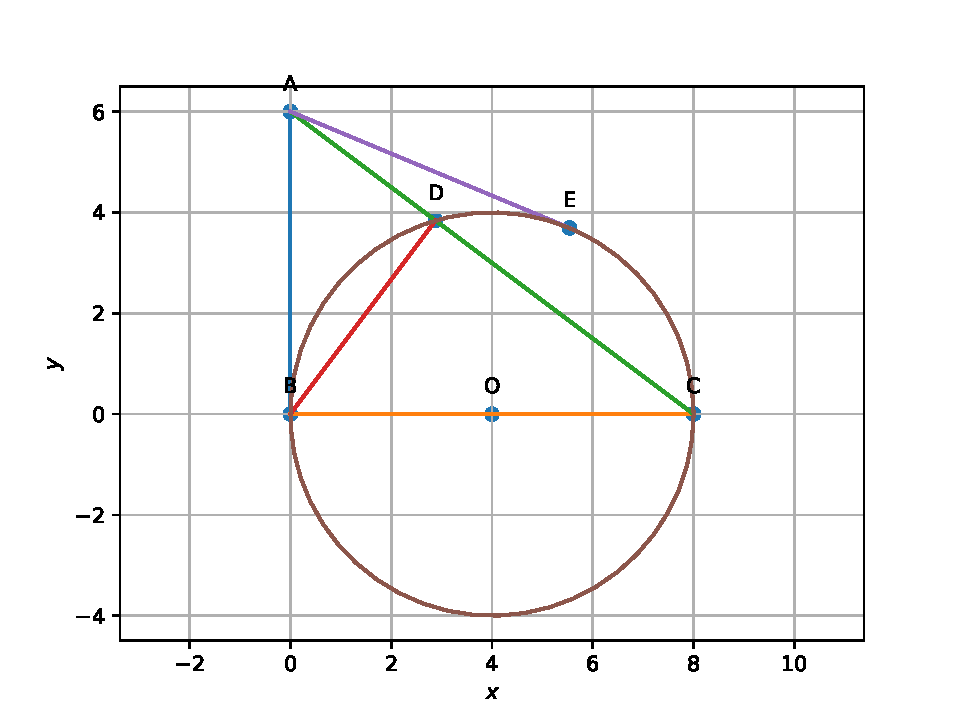
\includegraphics[width=\columnwidth]{chapters/10/11/2/6/figs/fig1.pdf}
		\caption{}
		\label{fig:10/11/2/6}
  	\end{figure}
\begin{align}
	BD &\perp AC
	\implies
	\vec{O} &= \frac{\vec{B}+\vec{C}}{2}
\label{eq3}
\end{align}
From 
	\eqref{eq:normal_line_foot}, the coordinates of $\vec{D}$ can be obtained.
\iffalse

\section*{\large Solution}

\begin{figure}[H]
\centering
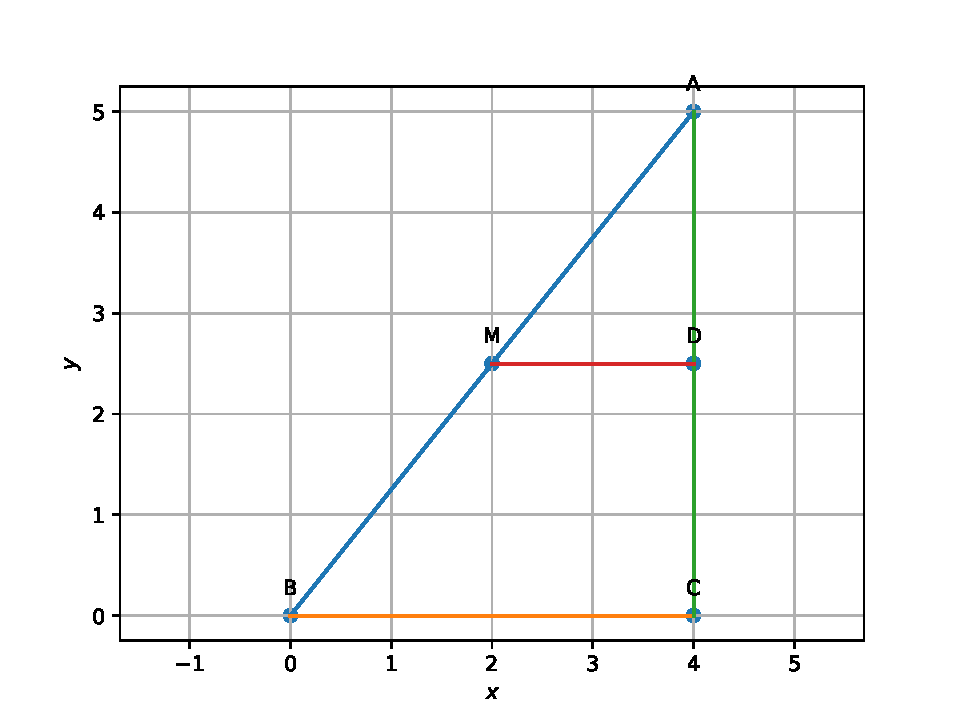
\includegraphics[width=1\columnwidth]{figs/fig1.pdf}
\caption{Tangents from A to circle through B, C and D}
\label{fig:triangle}
\end{figure}

Given that BD $\perp$ AC, which implies
\begin{equation}
\angle D = 90^\circ. 
\label{eq1}
\end{equation}

So, D can be found as the foot of the perpendicular from B on line AC. This is given by
\begin{equation}
\vec{D} = \vec{A} + \frac{\vec{m}^T(\vec{B-A})}{\norm{\vec{m}}^2}\vec{m} 
\label{eq2}
\end{equation}
where $\vec{m}$ is the direction vector for line AC.

The chord BC of the circle subtends $90^\circ$ at D. By the inclusive angle theorem, BC is the diameter of the circle with center O given by
\begin{equation}
\vec{O} = \frac{\vec{B}+\vec{C}}{2}
\label{eq3}
\end{equation}

In order to find the intersection points E and B of tangents from A, the origin is shifted from B to O. The equation of the circle in the new frame is
\begin{equation}
	\vec{x}^T\vec{x} = r^2
	\label{eq4}
\end{equation}

Let the the point of intersection between the tangent from A and the circle be P. Since P lies on the circle given by (\ref{eq4}) it is of the form    
\begin{equation}
	\vec{P} = \myvec{t \\ \sqrt{r^2-t^2}}
	\label{eq5}
\end{equation}

Since AP is a tangent to the circle, OP $\perp$ AP. This implies that
\begin{equation}
	(\vec{A}-\vec{P})^T(\vec{P}-\vec{O}) = 0
	\label{eq6}
\end{equation}

Since O is the origin in the new frame, $\vec{O} = \vec{0}$. Expanding (\ref{eq6}), we get 
\begin{equation}
	\vec{A}^T\vec{P} = \vec{P}^T\vec{P}
	\label{eq7}
\end{equation}

Substituting value of $\vec{P}$ from (\ref{eq5}) in (\ref{eq7}), we get
\begin{equation}
	\vec{A}^T\myvec{t \\ \sqrt{r^2-t^2}} = r^2	
	\label{eq8}
\end{equation}
Expanding and rearranging terms in \eqref{eq8}
\begin{multline}
	\norm{\vec{A}}^2t^2-2r^2\vec{e}_1^\top\vec{A}t+r^2(r^2-(\vec{e}_2^\top\vec{A})^2) = 0
	\label{eq:quad_t}
\end{multline}
Which is a quadratic equation in $t$ with roots given by
\begin{align}
	t = \frac{r^2\vec{e}_1^\top\vec{A}\pm\sqrt{r^4\vec{e}_1^\top\vec{A}^2-r^2\norm{\vec{A}}^2(r^2-\vec{e}_2^\top\vec{A}^2)}}{\norm{\vec{A}}^2}
	\label{eq:quad_soln}
\end{align}
Substituting the values of t from \eqref{eq:quad_soln} in \eqref{eq5} the two points of contact are obtained say $\vec{E_O}$ and $\vec{B_O}$.\\

The coordinates for position vectors $\vec{E_O}$ and $\vec{B_O}$ are with respect to origin O. The actual coordinates with respect to origin B is given by 
\begin{eqnarray}
	\vec{E} = \vec{E_O} + \vec{O}\\
	\vec{B} = \vec{B_O} + \vec{O}
\end{eqnarray}

\section*{\large Construction}
The input parameters are the lengths
\begin{eqnarray*}
	AB = a = 6\\
	BC = b = 8
\end{eqnarray*}
{
\setlength\extrarowheight{5pt}
\begin{tabular}{|c|c|c|}
	\hline
	\textbf{Symbol}&\textbf{Value}&\textbf{Description}\\
	\hline
	a&6&AB\\
	\hline
	b&8&BC\\
	\hline
	r&$\frac{b}{2}$&Radius\\
	\hline
	$\vec{m}$&$\vec{A-C}$&Direction vector of line AC\\
	\hline
	$\vec{D}$&$\vec{A} + \frac{\vec{m}^T(\vec{B-A})}{\norm{\vec{m}}^2}\vec{m}$&Point D\\[5pt]
	\hline
	$\vec{A_O}$&$\vec{A-O}$&$\vec{A}$ when origin shifted to $\vec{O}$\\
	\hline
	$t_1,t_2$&evaluate \eqref{eq:quad_soln}&solution of \eqref{eq:quad_t}\\[5pt] 
	\hline
	$\vec{E}$&$\myvec{t_1 \\ \sqrt{r^2-t_1^2}}+\vec{O}$&Point E\\[5pt]
	\hline
	$\vec{B}$&$\myvec{t_2 \\ \sqrt{r^2-t_2^2}}+\vec{O}$&Point B\\[5pt]
	\hline
\end{tabular}
}

\section*{\large Proofs}
\subsection*{\normalsize Foot of perpendicular from point $\vec{P}$ on line $\vec{A}+\lambda\vec{m}$}
Let the intersection point be $\vec{X}$. Since X is foot of perpendicular from point P to line with direction vector $\vec{m}$,
\begin{equation}
	\vec{m}^T(\vec{X-P}) = 0
	\label{pf1-eq-1}
\end{equation}
Since X lies on the line with direction vector $\vec{m}$,
\begin{equation}
	\vec{X} = \vec{A}+\lambda\vec{m}
	\label{pf1-eq-2}
\end{equation}
Substituting (\ref{pf1-eq-2}) in (\ref{pf1-eq-1}) and solving for $\lambda$,
\begin{equation}
	\lambda = \frac{\vec{m}^T(\vec{P-A})}{\norm{\vec{m}}^2}
	\label{pf1-eq-3}
\end{equation}
Substituting (\ref{pf1-eq-3}) in (\ref{pf1-eq-2}),
\begin{equation}
\vec{X} = \vec{A} + \frac{\vec{m}^T(\vec{P-A})}{\norm{\vec{m}}^2}\vec{m} 
\end{equation}

\subsection*{\normalsize Inclusive angle theorem}
The inclusive angle theorem states that the angle subtended by any chord at the center of a circle is twice the angle angle subtended by the same chord at any other point on the major segment. Take three points A, B, and C on a unit circle at angles $\theta$, $\phi$ and $\psi$. Then,
\begin{eqnarray}
	\vec{A} = \myvec{cos\theta\\sin\theta},
	\vec{B} = \myvec{cos\phi\\sin\phi},
	\vec{C} = \myvec{cos\psi\\sin\psi}
\end{eqnarray}

Let AB be the chord that subtends angles at the center O and at point C. The cosine of the angle subtended at point C is given by
\begin{align}
	cos(\angle ACB) = \frac{\langle A-C, B-C\rangle}{|A-C||B-C|}
	\label{pf2-eq-1}
\end{align}

Where
\begin{multline*}
	\langle A-C, B-C\rangle = \langle (\cos\theta-\cos\psi,\sin\theta-\sin\psi),(\cos\phi-\cos\psi,\\
	\sin\phi-\sin\psi)\rangle
	\end{multline*}
\begin{multline*}
	= (\cos\theta-\cos\psi)(\cos\phi-\cos\psi)+(\sin\theta-\sin\psi)\\
	(\sin\phi-\sin\psi)
\end{multline*}
\begin{multline*}
	= -2\sin\frac{\theta-\psi}2\sin\frac{\theta+\psi}2 \cdot(-2)\sin\frac{\phi-\psi}2\sin\frac{\phi+\psi}2 \\\quad+ 2\cos\frac{\theta+\psi}2\sin\frac{\theta-\psi}2 \cdot 2\cos\frac{\phi+\psi}2\sin\frac{\phi-\psi}2
\end{multline*}
\begin{multline*}
	= 4\sin\frac{\theta-\psi}2\sin\frac{\phi-\psi}2(\sin\frac{\theta+\psi}2\sin\frac{\phi+\psi}2+\\
	\cos\frac{\theta+\psi}2\cos\frac{\phi+\psi}2)
\end{multline*}
\begin{align*}
	= 4\sin\frac{\theta-\psi}2\sin\frac{\phi-\psi}2\cos\left(\frac{\theta+\psi}2-\frac{\phi+\psi}2\right)
\end{align*}
\begin{align}
	= 4\sin\frac{\theta-\psi}2\sin\frac{\phi-\psi}2\cos\frac{\theta-\phi}2
	\label{pf2-eq-2}
\end{align}

\begin{multline*}
	|A-C|^2|B-C|^2 = ((\cos\theta-\cos\psi)^2+(\sin\theta-\sin\psi)^2)\\
	((\cos\phi-\cos\psi)^2+(\sin\phi-\sin\psi)^2)
\end{multline*}
\begin{multline*}
	= (2-2\cos\theta\cos\psi - 2\sin\theta\sin\psi)(2-\\
	2\cos\phi\cos\psi - 2\sin\phi\sin\psi)
\end{multline*}
\begin{align*}
	&= 4(1-\cos(\theta-\psi))(1-\cos(\phi-\psi))\\
	&= 4\cdot 2\sin^2\frac{\theta-\psi}2\cdot 2\sin^2\frac{\phi-\psi}2
\end{align*}
\begin{align}
	&= 16 \sin^2\frac{\theta-\psi}2\sin^2\frac{\phi-\psi}2
	\label{pf2-eq-3}
\end{align}

Substituting (\ref{pf2-eq-2}) and (\ref{pf2-eq-3}) in (\ref{pf2-eq-1}),
\begin{equation}
	cos(\angle ACB) = cos(\frac{\theta-\phi}{2})	
\end{equation}
Hence $\angle ACB = \frac{\theta-\phi}{2} = \frac{\angle AOB}{2}$

\end{document}
\fi

\item A tangent $PQ$ at a point of a circle of radius 5cm meets a line through the centre $O$ at a point $Q$ so that $OQ$=12cm then length of $PQ$ is
\label{chapters/10/10/1/3}
\\
\solution
\iffalse
\documentclass[12pt]{article}
\usepackage{graphicx}
%\documentclass[journal,12pt,twocolumn]{IEEEtran}
\usepackage[none]{hyphenat}
\usepackage{graphicx}
\usepackage{gensymb}
\usepackage{listings}
\usepackage[english]{babel}
\usepackage{graphicx}
\usepackage{caption}
\usepackage[parfill]{parskip}
\usepackage{hyperref}
\usepackage{booktabs}
%\usepackage{setspace}\doublespacing\pagestyle{plain}
\def\inputGnumericTable{}
\usepackage{color}                                            %%
    \usepackage{array}                                            %%
    \usepackage{longtable}                                        %%
    \usepackage{calc}                                             %%
    \usepackage{multirow}                                         %%
    \usepackage{hhline}                                           %%
    \usepackage{ifthen}
\usepackage{array}
\usepackage{amsmath}   % for having text in math mode
\usepackage{parallel,enumitem}
\usepackage{listings}
\lstset{
language=tex,
frame=single,
breaklines=true
}
 
%Following 2 lines were added to remove the blank page at the beginning
\usepackage{atbegshi}% http://ctan.org/pkg/atbegshi
\AtBeginDocument{\AtBeginShipoutNext{\AtBeginShipoutDiscard}}
%
%New macro definitions
\newcommand{\mydet}[1]{\ensuremath{\begin{vmatrix}#1\end{vmatrix}}}
\providecommand{\brak}[1]{\ensuremath{\left(#1\right)}}
\providecommand{\norm}[1]{\left\lVert#1\right\rVert}
\newcommand{\solution}{\noindent \textbf{Solution: }}
\newcommand{\myvec}[1]{\ensuremath{\begin{pmatrix}#1\end{pmatrix}}}
\let\vec\mathbf
\begin{document}
\begin{center}
\enlargethispage{-4cm}
\title{\textbf{Three Dimensional Geometry}}
\date{\vspace{-5ex}} %Not to print date automatically
\maketitle
\end{center}
\setcounter{page}{1}
\section*{12$^{th}$ Maths - Chapter 11}
This is Problem-3 from Exercise 11.1
\begin{enumerate}

\solution
\fi
The input parameters are available in Table \ref{tab:chapters/10/10/1/3/}.
\begin{table}[ht!]\centering
%%%%%%%%%%%%%%%%%%%%%%%%%%%%%%%%%%%%%%%%%%%%%%%%%%%%%%%%%%%%%%%%%%%%%%
%%                                                                  %%
%%  This is the header of a LaTeX2e file exported from Gnumeric.    %%
%%                                                                  %%
%%  This file can be compiled as it stands or included in another   %%
%%  LaTeX document. The table is based on the longtable package so  %%
%%  the longtable options (headers, footers...) can be set in the   %%
%%  preamble section below (see PRAMBLE).                           %%
%%                                                                  %%
%%  To include the file in another, the following two lines must be %%
%%  in the including file:                                          %%
%%        \def\inputGnumericTable{}                                 %%
%%  at the beginning of the file and:                               %%
%%        \input{name-of-this-file.tex}                             %%
%%  where the table is to be placed. Note also that the including   %%
%%  file must use the following packages for the table to be        %%
%%  rendered correctly:                                             %%
%%    \usepackage[latin1]{inputenc}                                 %%
%%    \usepackage{color}                                            %%
%%    \usepackage{array}                                            %%
%%    \usepackage{longtable}                                        %%
%%    \usepackage{calc}                                             %%
%%    \usepackage{multirow}                                         %%
%%    \usepackage{hhline}                                           %%
%%    \usepackage{ifthen}                                           %%
%%  optionally (for landscape tables embedded in another document): %%
%%    \usepackage{lscape}                                           %%
%%                                                                  %%
%%%%%%%%%%%%%%%%%%%%%%%%%%%%%%%%%%%%%%%%%%%%%%%%%%%%%%%%%%%%%%%%%%%%%%



%%  This section checks if we are begin input into another file or  %%
%%  the file will be compiled alone. First use a macro taken from   %%
%%  the TeXbook ex 7.7 (suggestion of Han-Wen Nienhuys).            %%
\def\ifundefined#1{\expandafter\ifx\csname#1\endcsname\relax}


%%  Check for the \def token for inputed files. If it is not        %%
%%  defined, the file will be processed as a standalone and the     %%
%%  preamble will be used.                                          %%
\ifundefined{inputGnumericTable}

%%  We must be able to close or not the document at the end.        %%
	\def\gnumericTableEnd{\end{document}}


%%%%%%%%%%%%%%%%%%%%%%%%%%%%%%%%%%%%%%%%%%%%%%%%%%%%%%%%%%%%%%%%%%%%%%
%%                                                                  %%
%%  This is the PREAMBLE. Change these values to get the right      %%
%%  paper size and other niceties.                                  %%
%%                                                                  %%
%%%%%%%%%%%%%%%%%%%%%%%%%%%%%%%%%%%%%%%%%%%%%%%%%%%%%%%%%%%%%%%%%%%%%%

	\documentclass[12pt%
			  %,landscape%
                    ]{report}
       \usepackage[latin1]{inputenc}
       \usepackage{fullpage}
       \usepackage{color}
       \usepackage{array}
       \usepackage{longtable}
       \usepackage{calc}
       \usepackage{multirow}
       \usepackage{hhline}
       \usepackage{ifthen}

	\begin{document}


%%  End of the preamble for the standalone. The next section is for %%
%%  documents which are included into other LaTeX2e files.          %%
\else

%%  We are not a stand alone document. For a regular table, we will %%
%%  have no preamble and only define the closing to mean nothing.   %%
    \def\gnumericTableEnd{}

%%  If we want landscape mode in an embedded document, comment out  %%
%%  the line above and uncomment the two below. The table will      %%
%%  begin on a new page and run in landscape mode.                  %%
%       \def\gnumericTableEnd{\end{landscape}}
%       \begin{landscape}


%%  End f the else clause for this file being \input.              %%
\fi

%%%%%%%%%%%%%%%%%%%%%%%%%%%%%%%%%%%%%%%%%%%%%%%%%%%%%%%%%%%%%%%%%%%%%%
%%                                                                  %%
%%  The rest is the gnumeric table, except for the closing          %%
%%  statement. Changes below will alter the table's appearance.     %%
%%                                                                  %%
%%%%%%%%%%%%%%%%%%%%%%%%%%%%%%%%%%%%%%%%%%%%%%%%%%%%%%%%%%%%%%%%%%%%%%

\providecommand{\gnumericmathit}[1]{#1} 
%%  Uncomment the next line if you would like your numbers to be in %%
%%  italics if they are italizised in the gnumeric table.           %%
%\renewcommand{\gnumericmathit}[1]{\mathit{#1}}
\providecommand{\gnumericPB}[1]%
{\let\gnumericTemp=\\#1\let\\=\gnumericTemp\hspace{0pt}}
 \ifundefined{gnumericTableWidthDefined}
        \newlength{\gnumericTableWidth}
        \newlength{\gnumericTableWidthComplete}
        \newlength{\gnumericMultiRowLength}
        \global\def\gnumericTableWidthDefined{}
 \fi
%% The following setting protects this code from babel shorthands.  %%
 \ifthenelse{\isundefined{\languageshorthands}}{}{\languageshorthands{english}}
%%  The default table format retains the relative column widths of  %%
%%  gnumeric. They can easily be changed to c, r or l. In that case %%
%%  you may want to comment out the next line and uncomment the one %%
%%  thereafter                                                      %%
\providecommand\gnumbox{\makebox[0pt]}
%%\providecommand\gnumbox[1][]{\makebox}

%% to adjust positions in multirow situations                       %%
\setlength{\bigstrutjot}{\jot}
\setlength{\extrarowheight}{\doublerulesep}

%%  The \setlongtables command keeps column widths the same across  %%
%%  pages. Simply comment out next line for varying column widths.  %%
\setlongtables

\setlength\gnumericTableWidth{%
	53pt+%
	53pt+%
	82pt+%
	53pt+%
0pt}
\def\gumericNumCols{4}
\setlength\gnumericTableWidthComplete{\gnumericTableWidth+%
         \tabcolsep*\gumericNumCols*2+\arrayrulewidth*\gumericNumCols}
\ifthenelse{\lengthtest{\gnumericTableWidthComplete > \linewidth}}%
         {\def\gnumericScale{1*\ratio{\linewidth-%
                        \tabcolsep*\gumericNumCols*2-%
                        \arrayrulewidth*\gumericNumCols}%
{\gnumericTableWidth}}}%
{\def\gnumericScale{1}}

%%%%%%%%%%%%%%%%%%%%%%%%%%%%%%%%%%%%%%%%%%%%%%%%%%%%%%%%%%%%%%%%%%%%%%
%%                                                                  %%
%% The following are the widths of the various columns. We are      %%
%% defining them here because then they are easier to change.       %%
%% Depending on the cell formats we may use them more than once.    %%
%%                                                                  %%
%%%%%%%%%%%%%%%%%%%%%%%%%%%%%%%%%%%%%%%%%%%%%%%%%%%%%%%%%%%%%%%%%%%%%%

\ifthenelse{\isundefined{\gnumericColA}}{\newlength{\gnumericColA}}{}\settowidth{\gnumericColA}{\begin{tabular}{@{}p{53pt*\gnumericScale}@{}}x\end{tabular}}
\ifthenelse{\isundefined{\gnumericColB}}{\newlength{\gnumericColB}}{}\settowidth{\gnumericColB}{\begin{tabular}{@{}p{53pt*\gnumericScale}@{}}x\end{tabular}}
\ifthenelse{\isundefined{\gnumericColC}}{\newlength{\gnumericColC}}{}\settowidth{\gnumericColC}{\begin{tabular}{@{}p{82pt*\gnumericScale}@{}}x\end{tabular}}
\ifthenelse{\isundefined{\gnumericColD}}{\newlength{\gnumericColD}}{}\settowidth{\gnumericColD}{\begin{tabular}{@{}p{53pt*\gnumericScale}@{}}x\end{tabular}}

	\begin{center}
\begin{tabular}[c]{%
	b{\gnumericColA}%
	b{\gnumericColB}%
	b{\gnumericColC}%
	b{\gnumericColD}%
	}

%%%%%%%%%%%%%%%%%%%%%%%%%%%%%%%%%%%%%%%%%%%%%%%%%%%%%%%%%%%%%%%%%%%%%%
%%  The longtable options. (Caption, headers... see Goosens, p.124) %%
%	\caption{The Table Caption.}             \\	%
% \hline	% Across the top of the table.
%%  The rest of these options are table rows which are placed on    %%
%%  the first, last or every page. Use \multicolumn if you want.    %%

%%  Header for the first page.                                      %%
%	\multicolumn{4}{c}{The First Header} \\ \hline 
%	\multicolumn{1}{c}{colTag}	%Column 1
%	&\multicolumn{1}{c}{colTag}	%Column 2
%	&\multicolumn{1}{c}{colTag}	%Column 3
%	&\multicolumn{1}{c}{colTag}	\\ \hline %Last column
%	\endfirsthead

%%  The running header definition.                                  %%
%	\hline
%	\multicolumn{4}{l}{\ldots\small\slshape continued} \\ \hline
%	\multicolumn{1}{c}{colTag}	%Column 1
%	&\multicolumn{1}{c}{colTag}	%Column 2
%	&\multicolumn{1}{c}{colTag}	%Column 3
%	&\multicolumn{1}{c}{colTag}	\\ \hline %Last column
%	\endhead

%%  The running footer definition.                                  %%
%	\hline
%	\multicolumn{4}{r}{\small\slshape continued\ldots} \\
%	\endfoot

%%  The ending footer definition.                                   %%
%	\multicolumn{4}{c}{That's all folks} \\ \hline 
%	\endlastfoot
%%%%%%%%%%%%%%%%%%%%%%%%%%%%%%%%%%%%%%%%%%%%%%%%%%%%%%%%%%%%%%%%%%%%%%

\hhline{|-|-|-~}
	 \multicolumn{1}{|p{\gnumericColA}|}%
	{\gnumericPB{\centering}\gnumbox{\textbf{Symbol}}}
	&\multicolumn{1}{p{\gnumericColB}|}%
	{\gnumericPB{\centering}\gnumbox{\textbf{Value}}}
	&\multicolumn{1}{p{\gnumericColC}|}%
	{\gnumericPB{\centering}\gnumbox{\textbf{Description}}}
	&
\\
\hhline{|---|~}
	 \multicolumn{1}{|p{\gnumericColA}|}%
	{\gnumericPB{\centering}\gnumbox{$r$}}
	&\multicolumn{1}{p{\gnumericColB}|}%
	{\gnumericPB{\centering}\gnumbox{${5}$}}
	&\multicolumn{1}{p{\gnumericColC}|}%
	{\gnumericPB{\centering}\gnumbox{Radius}}
	&
\\
\hhline{|---|~}
	 \multicolumn{1}{|p{\gnumericColA}|}%
	{\gnumericPB{\centering}\gnumbox{$\vec{O}$}}
	&\multicolumn{1}{p{\gnumericColB}|}%
	{\gnumericPB{\centering}\gnumbox{$\myvec{0 \\ 0}$}}
	&\multicolumn{1}{p{\gnumericColC}|}%
	{\gnumericPB{\centering}\gnumbox{Centre $\vec{O}$}}
	&
\\
\hhline{|---|~}
	 \multicolumn{1}{|p{\gnumericColA}|}%
	{\gnumericPB{\centering}\gnumbox{$\vec{P}$}}
	&\multicolumn{1}{p{\gnumericColB}|}%
	{\gnumericPB{\centering}\gnumbox{$r\myvec{\cos{\theta}\\\sin{\theta}}$}}
	&\multicolumn{1}{p{\gnumericColC}|}%
	{\gnumericPB{\centering}\gnumbox{Point of contact}}
	&
\\
\hhline{|---|~}
	 \multicolumn{1}{|p{\gnumericColA}|}%
	{\gnumericPB{\centering}\gnumbox{$d$}}
	&\multicolumn{1}{p{\gnumericColB}|}%
	{\gnumericPB{\centering}\gnumbox{12}}
	&\multicolumn{1}{p{\gnumericColC}|}%
	{\gnumericPB{\centering}\gnumbox{Lenght of $OQ$}}
	&
\\
\hhline{|-|-|-|~}
\end{tabular}
	\end{center}

\ifthenelse{\isundefined{\languageshorthands}}{}{\languageshorthands{\languagename}}
\gnumericTableEnd

\caption{}
\label{tab:chapters/10/10/1/3/} 
\end{table}
From the given information, 	
\begin{align}
	\norm{\vec{Q}}^2&=d^2\label{eq:chapters/10/10/1/3/1}
	\\
\brak{\vec{Q}-\vec{P}}^{\top}\vec{P}&=0 \implies
\vec{P}^{\top}\vec{Q}=\norm{\vec{P}}^2=r^2\\
	\text{or, }	\vec{P}^{\top}\vec{Q}&=25\label{eq:chapters/10/10/1/3/4}
\end{align}
For $\theta=0\degree$ 
\begin{align}
\vec{P}=\myvec{5\\0}
\end{align}
Substituting the above in \eqref{eq:chapters/10/10/1/3/4},
\begin{align}
\myvec{5&0}\vec{Q}&=25\\
\implies 
	\vec{Q}&=\myvec{5\\0}+\mu\myvec{0\\1}\label{eq:chapters/10/10/1/3/9}
\end{align}
	which is of the form 
\begin{align}
	\vec{Q}=\vec{A}+\mu\vec{m}\label{eq:chapters/10/10/1/3/10}
\end{align}
		Then substituting \eqref{eq:chapters/10/10/1/3/10} in \eqref{eq:chapters/10/10/1/3/1} yeilds,
\begin{align}
	&\implies\brak{\vec{A}+\mu\vec{m}}^{\top}\brak{\vec{A}+\mu\vec{m}}=d^2\\
	&\implies \mu^2\norm{\vec{m}}^2+2\mu\vec{A}^{\top}\vec{m}+\norm{\vec{A}}^2=d^2\label{eq:chapters/10/10/1/3/14}
\end{align}
where
\begin{align}
	\vec{A}=\myvec{5\\0}\text{ and }\vec{m}=\myvec{0\\1}
\end{align}
	Substituting numerical values, 
\begin{align}
\mu^2=119
	\implies\mu=\pm\sqrt{119}
\end{align}
yeilding 
\begin{align}
\vec{Q_1}=\myvec{5\\\sqrt{119}},\vec{Q_2}=\myvec{5\\-\sqrt{119}}
\end{align}
Thus, 
\begin{align}
	PQ_1 = PQ_2  = \sqrt{119}
\end{align}
See Fig. 
\ref{fig:chapters/10/10/1/3/Fig1}.
\begin{figure}[!h]
\begin{center}
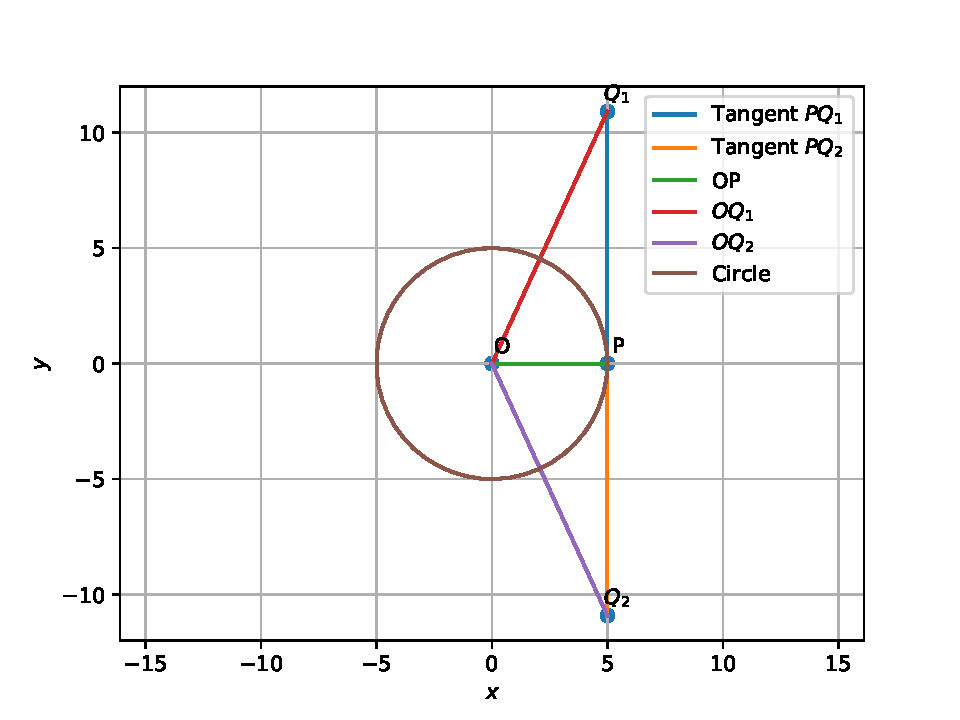
\includegraphics[width=\columnwidth]{chapters/10/10/1/3/figs/fig2.pdf}
\end{center}
\caption{}
\label{fig:chapters/10/10/1/3/Fig1}
\end{figure}

\item 
\label{chapters/10/10/1/4}
\iffalse
\def\mytitle{MATRICES USING PYTHON}
\def\myauthor{THOUTU RAHUL RAJ}
\def\contact{rdj4648@gmail.com}
\def\mymodule{Future Wireless Communication (FWC)}
\documentclass[10pt, a4paper]{article}
\usepackage[a4paper,outer=1.5cm,inner=1.5cm,top=1.75cm,bottom=1.5cm]{geometry}
\twocolumn
\usepackage{graphicx}
\graphicspath{{./images/}}
\usepackage[colorlinks,linkcolor={black},citecolor={blue!80!black},urlcolor={blue!80!black}]{hyperref}
\usepackage[parfill]{parskip}
\usepackage{lmodern}
\usepackage{amsmath,amsfonts,amssymb,amsthm}
\usepackage{tikz}
	\usepackage{physics}
%\documentclass[tikz, border=2mm]{standalone}
\usepackage{karnaugh-map}
%\documentclass{article}
\usepackage{tabularx}
\usepackage{circuitikz}
\usetikzlibrary{calc}
\usepackage{amsmath}
\usepackage{amssymb}
\renewcommand*\familydefault{\sfdefault}
\usepackage{watermark}
\usepackage{lipsum}
\usepackage{xcolor}
\usepackage{listings}
\usepackage{float}
\usepackage{titlesec}
\providecommand{\norm}[1]{\left\lVert#1\right\rVert}
\providecommand{\sbrak}[1]{\ensuremath{{}\left[#1\right]}}
\providecommand{\lsbrak}[1]{\ensuremath{{}\left[#1\right.}}
\providecommand{\rsbrak}[1]{\ensuremath{{}\left.#1\right]}}
\providecommand{\brak}[1]{\ensuremath{\left(#1\right)}}
\providecommand{\lbrak}[1]{\ensuremath{\left(#1\right.}}
\providecommand{\rbrak}[1]{\ensuremath{\left.#1\right)}}
\providecommand{\cbrak}[1]{\ensuremath{\left\{#1\right\}}}
\providecommand{\lcbrak}[1]{\ensuremath{\left\{#1\right.}}
\providecommand{\rcbrak}[1]{\ensuremath{\left.#1\right\}}}
\newcommand{\myvec}[1]{\ensuremath{\begin{pmatrix}#1\end{pmatrix}}}
\let\vec\mathbf
\providecommand{\mtx}[1]{\mathbf{#1}}
\titlespacing{\subsection}{1pt}{\parskip}{3pt}
\titlespacing{\subsubsection}{0pt}{\parskip}{-\parskip}
\titlespacing{\paragraph}{0pt}{\parskip}{\parskip}
\newcommand{\figuremacro}[5]

\begin{document}

\title{\mytitle}
\author{\myauthor\hspace{1em}\\\contact\\FWC22008\hspace{6.5em}IITH\hspace{0.5em}\mymodule\hspace{6em}ASSIGN-5}
\date{}
	\maketitle
		
	\tableofcontents
\vspace{5mm}
   \section{Problem}
\textbf{ 
   \fi
Draw a circle and two lines parallel to a given line such that one is a tangent and the other is a secant to the circle 
	\begin{figure}[!h]
		\centering
 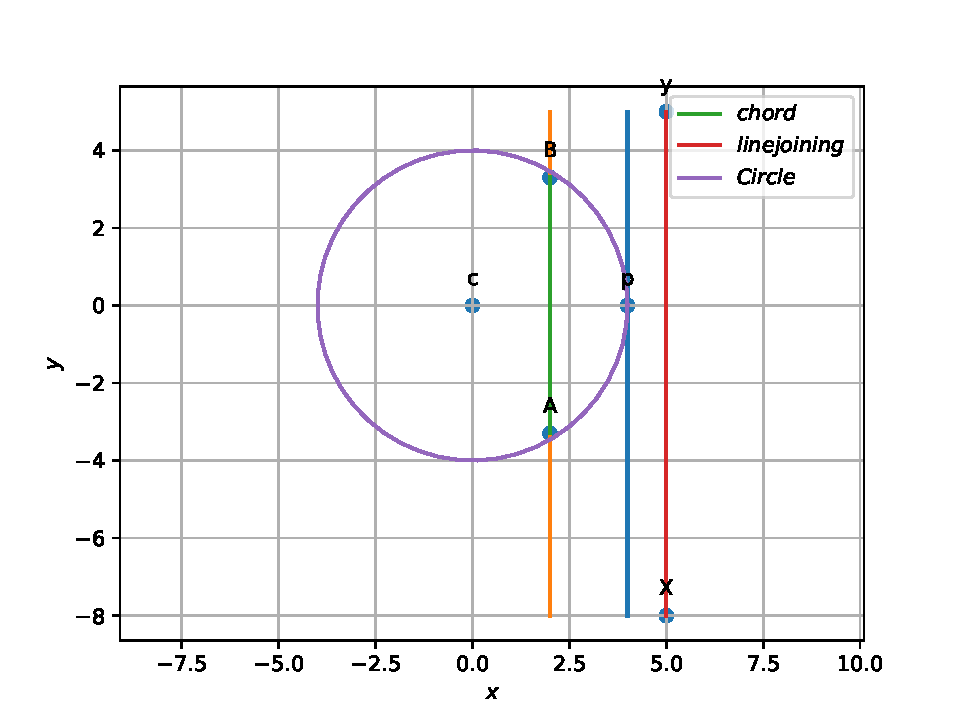
\includegraphics[width=\columnwidth]{chapters/10/10/1/4/figs/fig.pdf}
		\caption{}
		\label{fig:10/10/1/4}
  	\end{figure}
	\\
	\solution	
\iffalse
 \section{Construction}
 	\begin{center}
     Figure of Construction
     \includegraphics[scale=0.5]{figs/fig.pdf} 
  	\end{center}
  	The input parameters for this construction are 
\begin{center}
\begin{tabular}{|c|c|c|}
	\hline
	\textbf{Symbol}&\textbf{Value}&\textbf{Description}\\
	\hline
	r&4&Radius of the circle\\
	\hline		
	c&5&constant \\
	\hline
	\textbf{C}&$\
	\begin{pmatrix}
		0 \\
		0 \\
	\end{pmatrix}$
	&center\\
	\hline
	
\end{tabular}
\end{center}

   \section{Solution}

\vspace{1mm}
\textbf{Termux commands :}
\begin{lstlisting}
python3 xyz.py
\end{lstlisting}


\vspace{.25 cm}
\textbf{To Prove:}
In a given circle and a line draw two lines such that one is a secant and other one is tangent. 

 Given:
 \fi
 The parameters of the circle in Fig. 
		\ref{fig:10/10/1/4} are
%Circle center with (0,0), radius 4 and a line. \\
\begin{align}
%\vec{x}^{\top}\vec{V}\vec{x}+2\vec{u}^{\top}\vec{x}+f=0
	\vec{u} = \vec{0},
f = -16
\end{align}	
Considering the given line to be 
\begin{align}
\vec{e}_1^{\top}\vec{x}=5
\end{align}
the tangent to the circle will be 
\begin{align}
\vec{e}_1^{\top}\vec{x}=4
\end{align}
and the secant will be 
\begin{align}
\vec{e}_1^{\top}\vec{x}=c
\end{align}
%
where
\begin{align}
	\abs{c} < 4
\end{align}
\iffalse
and the secant will be 
\begin{align}
D = \pm C\\
\vec{D}= \pm \sqrt{e^2\brak{\vec{u}^{\top}\vec{n}}^2-\lambda_2\brak{e^2-1}\brak{\norm{\vec{u}}^2 - \lambda_2 f}}
\end{align}
by sloving the above eq we get,
\begin{align}
D = \pm 4 
\end{align}

and the condition for secant which is also parallel to the given line will be
\begin{align}
D \geq 0 
\end{align}
i.e 
\begin{align}
-4 < C < 4
\end{align}
\vspace{1mm}
The below python code realizes the above construction:	\\
\url{https://github.com/Rahulraj00/Assignments/tree/main/Assignments/assg_5/xyz.py}
\bibliographystyle{ieeetr}
\end{document}
\fi

\item From a point $\vec{Q}$, the length of the tangent to a circle is $24 cm$ and the distance of $\vec{Q}$ from the centre is $25 cm$. Find the radius of the circle. Draw the circle and the tangents. 
\label{chapters/10/10/2/1}
\\
\solution
\iffalse
\documentclass[12pt]{article}
\usepackage{graphicx}
\usepackage[none]{hyphenat}
\usepackage{graphicx}
\usepackage{listings}
\usepackage[english]{babel}
\usepackage{graphicx}
\usepackage{caption} 
\usepackage{booktabs}
\usepackage{array}
\usepackage{amssymb} % for \because
\usepackage{amsmath}   % for having text in math mode
\usepackage{extarrows} % for Row operations arrows
\usepackage{listings}
\lstset{
  frame=single,
  breaklines=true
}
\usepackage{hyperref}
\usepackage{mathtools}

%Following 2 lines were added to remove the blank page at the beginning
\usepackage{atbegshi}% http://ctan.org/pkg/atbegshi
\AtBeginDocument{\AtBeginShipoutNext{\AtBeginShipoutDiscard}}


%New macro definitions
\newcommand{\mydet}[1]{\ensuremath{\begin{vmatrix}#1\end{vmatrix}}}
\providecommand{\brak}[1]{\ensuremath{\left(#1\right)}}
\providecommand{\norm}[1]{\left\lVert#1\right\rVert}
\providecommand{\abs}[1]{\left\vert#1\right\vert}
\newcommand{\solution}{\noindent \textbf{Solution: }}
\newcommand{\myvec}[1]{\ensuremath{\begin{pmatrix}#1\end{pmatrix}}}
\let\vec\mathbf


\begin{document}

\begin{center}
\title{\textbf{Conic Sections - Circle}}
\date{\vspace{-5ex}} %Not to print date automatically
\maketitle
\end{center}
\setcounter{page}{1}

\section{10$^{th}$ Maths - Chapter 10}
This is Problem-1 from Exercise 10.2
\begin{enumerate}
\solution 
\fi
Let
\begin{align}
		\vec{Q} =\myvec{0 \\ 0}
\end{align}
and
$\vec{O}$ be the centre of the circle.  Let $\vec{R}_1 \text{ and } \vec{R}_2$ be the two points on the circle such that $R_1Q$ and $R_2Q$ are tangents to the circle from the point $\vec{Q}$. Given that,  
\begin{align}
	OQ &= 25, R_1Q = R_2Q = 24 \\ 
	\therefore \vec{O} &= \myvec{25 \\ 0} \\
	r &= OR_1 = \sqrt{OQ^2 - R_1Q^2}  \\
	&= \sqrt{25^2 - 24^2} \\
	&= 7
\end{align}
We have to find points $\vec{R}_1 \text{ and } \vec{R}_2$. 
We know that the equation to the circle is given as
\begin{align}
	\label{eq:chapters/10/10/2/1/circEq1}
	\norm{\vec{x}}^2+2\vec{x}^\top\vec{u}+f = 0 
\end{align}
where
\begin{align}
	\vec{u} &= -\vec{O}  = -\myvec{25\\0}\text{ and } \\
        \label{eq:chapters/10/10/2/1/fRelation}
	f &= \norm{\vec{O}}^2 - r^2 = 576
\end{align}
The matrix
\begin{align}
	\vec{\Sigma} &= \brak{\vec{Q}+\vec{u}}\brak{\vec{Q}+\vec{u}}^\top - \brak{\norm{\vec{Q}}^2+2\vec{u}^\top\vec{Q}+f}\vec{I}
	\\
  \begin{split}
	={}& \brak{\myvec{0\\0}-\myvec{25\\0}}\brak{\myvec{0\\0}-\myvec{25\\0}}^\top \\
	   & -\brak{0-2\myvec{25&0}\myvec{0 \\0}+576}\vec{I}\\ 
  \end{split}\\
	&= \myvec{-25\\0}\myvec{-25&0} - \brak{576}\vec{I} \\ 
	&= \myvec{625&0\\0&0 } - \myvec{576&0\\0&576} \\ 
        \label{eq:chapters/10/10/2/1/Eq1}
	&= \myvec{49&0\\0&-576 } 
\end{align}
From \eqref{eq:chapters/10/10/2/1/Eq1}, we can deduce Eigen pairs as follows 
\begin{align}
	\lambda_1 &= 49 , \lambda_2 = -576 \\
	\vec{p_1} &= \myvec{1\\0} , \vec{p_2} = \myvec{0\\1}
\end{align}
Then
\begin{align}
	\vec{n_1} &= \myvec{1&0\\0&1}\myvec{\sqrt{\abs{\lambda_1}} \\ \sqrt{\abs{\lambda_2}}} = \myvec{7\\24} \\
	\vec{n_2} &= \myvec{1&0\\0&1}\myvec{\sqrt{\abs{\lambda_1}} \\ -\sqrt{\abs{\lambda_2}}} = \myvec{7\\-24}
\end{align}
The points of contact of a tangent on a circle from an external point is given by 
\begin{align}
	\vec{q_{ij}} &= \brak{\pm r \frac{\vec{n_j}}{\norm{\vec{n_j}}}- \vec{u}},  \quad i,j = 1,2 \\
	\vec{q_{i1}} &= \brak{\pm r \frac{\vec{n_1}}{\norm{\vec{n_1}}}- \vec{u}} \\
	&= \brak{\pm \frac{7}{25}\myvec{7\\24}+ \myvec{25\\0}} \\
	&= \brak{\pm \myvec{\frac{49}{25} \\ \\[1pt] \frac{168}{25}} + \myvec{25\\0}} \\
	&= \myvec{\frac{674}{25} \\ \\[1pt] \frac{168}{25}}, \myvec{\frac{576}{25} \\ \\[1pt] -\frac{168}{25}}
\end{align}
\begin{align}
	\vec{q_{i2}} &= \brak{\pm r \frac{\vec{n_2}}{\norm{\vec{n_2}}}- \vec{u}} \\
	&= \brak{\pm \frac{7}{25}\myvec{7 \\ -24}+ \myvec{25 \\ 0}} \\
	&= \brak{\pm \myvec{\frac{49}{25} \\ \\[1pt] \frac{-168}{25}} + \myvec{25 \\ 0}} \\
	&= \myvec{\frac{674}{25} \\ \\[1pt] \frac{-168}{25}}, \myvec{\frac{576}{25} \\ \\[1pt] \frac{168}{25}}  \\
	\therefore \vec{R}_1 &= \vec{q}_{22} = \myvec{\frac{576}{25} \\ \\[1pt] \frac{168}{25}} \\
	\vec{R}_2 &= \vec{q}_{12} = \myvec{\frac{576}{25} \\ \\[1pt] -\frac{168}{25}}
\end{align}
The figure is as shown in \ref{fig:chapters/10/10/2/1/Fig1}
\begin{figure}[!h]
	\begin{center}
		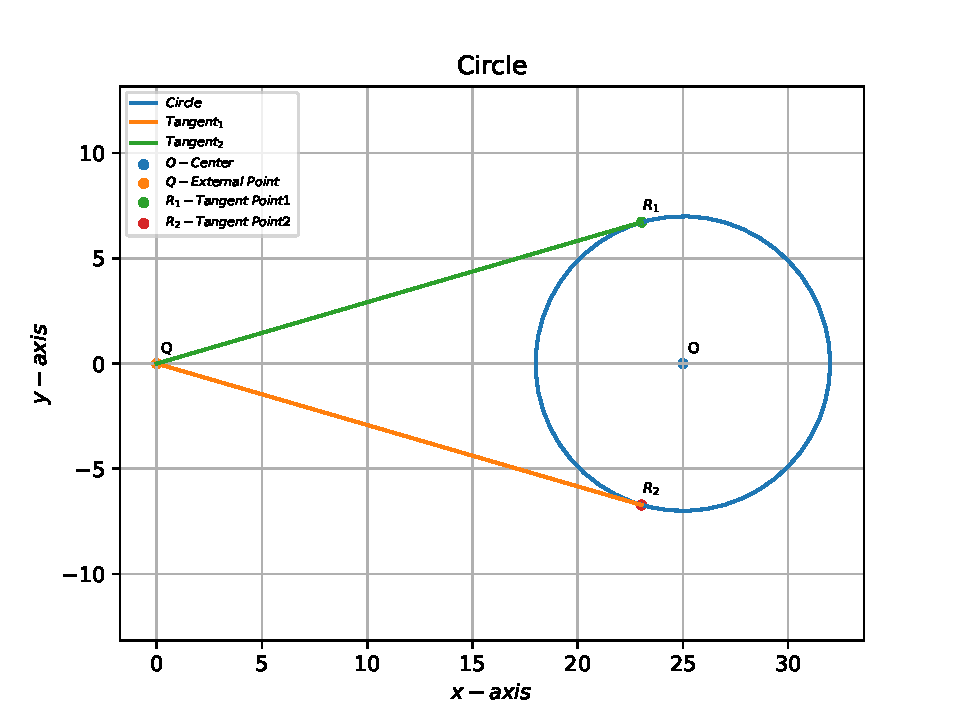
\includegraphics[width=\columnwidth]{chapters/10/10/2/1/figs/problem1.pdf}
	\end{center}
\caption{}
\label{fig:chapters/10/10/2/1/Fig1}
\end{figure}

\item In Fig. \ref{fig:chapters/10/10/2/2/Fig1}, if TP and TQ are two tangents to a circle with centre O so that $\angle{POQ} = 110\degree$ then find $\angle{PTQ}$. 
\\
\solution
\iffalse
\documentclass[12pt]{article}
\usepackage{graphicx}
\usepackage{amsmath}
\usepackage{mathtools}
\usepackage{gensymb}
\usepackage{tabularx}
\usepackage{array}
\usepackage[latin1]{inputenc}
\usepackage{fullpage}
\usepackage{color}
\usepackage{array}
\usepackage{longtable}
\usepackage{calc}
\usepackage{multirow}
\usepackage{hhline}
\usepackage{ifthen}
\usepackage{lscape}
\usepackage{float}

\newcommand{\mydet}[1]{\ensuremath{\begin{vmatrix}#1\end{vmatrix}}}
\providecommand{\brak}[1]{\ensuremath{\left(#1\right)}}
\providecommand{\norm}[1]{\left\lVert#1\right\rVert}
\providecommand{\abs}[1]{\left\vert#1\right\vert}
\newcommand{\solution}{\noindent \textbf{Solution: }}
\newcommand{\myvec}[1]{\ensuremath{\begin{pmatrix}#1\end{pmatrix}}}
\let\vec\mathbf

\def\inputGnumericTable{}

\begin{document}
\begin{center}
\textbf\large{TANGENTS AND NORMALS}

\end{center}
\section*{Excercise 10.2}

\solution
\fi
Let the output angle be $\phi$.
The input parameters are given as
%%%%%%%%%%%%%%%%%%%%%%%%%%%%%%%%%%%%%%%%%%%%%%%%%%%%%%%%%%%%%%%%%%%%%%
%%                                                                  %%
%%  This is the header of a LaTeX2e file exported from Gnumeric.    %%
%%                                                                  %%
%%  This file can be compiled as it stands or included in another   %%
%%  LaTeX document. The table is based on the longtable package so  %%
%%  the longtable options (headers, footers...) can be set in the   %%
%%  preamble section below (see PRAMBLE).                           %%
%%                                                                  %%
%%  To include the file in another, the following two lines must be %%
%%  in the including file:                                          %%
%%        \def\inputGnumericTable{}                                 %%
%%  at the beginning of the file and:                               %%
%%        \input{name-of-this-file.tex}                             %%
%%  where the table is to be placed. Note also that the including   %%
%%  file must use the following packages for the table to be        %%
%%  rendered correctly:                                             %%
%%    \usepackage[latin1]{inputenc}                                 %%
%%    \usepackage{color}                                            %%
%%    \usepackage{array}                                            %%
%%    \usepackage{longtable}                                        %%
%%    \usepackage{calc}                                             %%
%%    \usepackage{multirow}                                         %%
%%    \usepackage{hhline}                                           %%
%%    \usepackage{ifthen}                                           %%
%%  optionally (for landscape tables embedded in another document): %%
%%    \usepackage{lscape}                                           %%
%%                                                                  %%
%%%%%%%%%%%%%%%%%%%%%%%%%%%%%%%%%%%%%%%%%%%%%%%%%%%%%%%%%%%%%%%%%%%%%%



%%  This section checks if we are begin input into another file or  %%
%%  the file will be compiled alone. First use a macro taken from   %%
%%  the TeXbook ex 7.7 (suggestion of Han-Wen Nienhuys).            %%
\def\ifundefined#1{\expandafter\ifx\csname#1\endcsname\relax}


%%  Check for the \def token for inputed files. If it is not        %%
%%  defined, the file will be processed as a standalone and the     %%
%%  preamble will be used.                                          %%
\ifundefined{inputGnumericTable}

%%  We must be able to close or not the document at the end.        %%
	\def\gnumericTableEnd{\end{document}}


%%%%%%%%%%%%%%%%%%%%%%%%%%%%%%%%%%%%%%%%%%%%%%%%%%%%%%%%%%%%%%%%%%%%%%
%%                                                                  %%
%%  This is the PREAMBLE. Change these values to get the right      %%
%%  paper size and other niceties.                                  %%
%%                                                                  %%
%%%%%%%%%%%%%%%%%%%%%%%%%%%%%%%%%%%%%%%%%%%%%%%%%%%%%%%%%%%%%%%%%%%%%%

	\documentclass[12pt%
			  %,landscape%
                    ]{report}
       \usepackage[latin1]{inputenc}
       \usepackage{fullpage}
       \usepackage{color}
       \usepackage{amsmath}
       \usepackage{array}
       \usepackage{longtable}
       \usepackage{calc}
       \usepackage{multirow}
       \usepackage{hhline}
       \usepackage{ifthen}
       \let\vec\mathbf
\newcommand{\myvec}[1]{\ensuremath{\begin{pmatrix}#1\end{pmatrix}}}

	\begin{document}


%%  End of the preamble for the standalone. The next section is for %%
%%  documents which are included into other LaTeX2e files.          %%
\else

%%  We are not a stand alone document. For a regular table, we will %%
%%  have no preamble and only define the closing to mean nothing.   %%
    \def\gnumericTableEnd{}

%%  If we want landscape mode in an embedded document, comment out  %%
%%  the line above and uncomment the two below. The table will      %%
%%  begin on a new page and run in landscape mode.                  %%
%       \def\gnumericTableEnd{\end{landscape}}
%       \begin{landscape}


%%  End of the else clause for this file being \input.              %%
\fi

%%%%%%%%%%%%%%%%%%%%%%%%%%%%%%%%%%%%%%%%%%%%%%%%%%%%%%%%%%%%%%%%%%%%%%
%%                                                                  %%
%%  The rest is the gnumeric table, except for the closing          %%
%%  statement. Changes below will alter the table's appearance.     %%
%%                                                                  %%
%%%%%%%%%%%%%%%%%%%%%%%%%%%%%%%%%%%%%%%%%%%%%%%%%%%%%%%%%%%%%%%%%%%%%%

\providecommand{\gnumericmathit}[1]{#1} 
%%  Uncomment the next line if you would like your numbers to be in %%
%%  italics if they are italizised in the gnumeric table.           %%
%\renewcommand{\gnumericmathit}[1]{\mathit{#1}}
\providecommand{\gnumericPB}[1]%
{\let\gnumericTemp=\\#1\let\\=\gnumericTemp\hspace{0pt}}
 \ifundefined{gnumericTableWidthDefined}
        \newlength{\gnumericTableWidth}
        \newlength{\gnumericTableWidthComplete}
        \newlength{\gnumericMultiRowLength}
        \global\def\gnumericTableWidthDefined{}
 \fi
%% The following setting protects this code from babel shorthands.  %%
 \ifthenelse{\isundefined{\languageshorthands}}{}{\languageshorthands{english}}
%%  The default table format retains the relative column widths of  %%
%%  gnumeric. They can easily be changed to c, r or l. In that case %%
%%  you may want to comment out the next line and uncomment the one %%
%%  thereafter                                                      %%
\providecommand\gnumbox{\makebox[0pt]}
%%\providecommand\gnumbox[1][]{\makebox}

%% to adjust positions in multirow situations                       %%
\setlength{\bigstrutjot}{\jot}
\setlength{\extrarowheight}{\doublerulesep}

%%  The \setlongtables command keeps column widths the same across  %%
%%  pages. Simply comment out next line for varying column widths.  %%
\setlongtables

\setlength\gnumericTableWidth{%
	133pt+%
	53pt+%
	57pt+%
0pt}
\def\gumericNumCols{3}
\setlength\gnumericTableWidthComplete{\gnumericTableWidth+%
         \tabcolsep*\gumericNumCols*2+\arrayrulewidth*\gumericNumCols}
\ifthenelse{\lengthtest{\gnumericTableWidthComplete > \linewidth}}%
         {\def\gnumericScale{\ratio{\linewidth-%
                        \tabcolsep*\gumericNumCols*2-%
                        \arrayrulewidth*\gumericNumCols}%
{\gnumericTableWidth}}}%
{\def\gnumericScale{1}}

%%%%%%%%%%%%%%%%%%%%%%%%%%%%%%%%%%%%%%%%%%%%%%%%%%%%%%%%%%%%%%%%%%%%%%
%%                                                                  %%
%% The following are the widths of the various columns. We are      %%
%% defining them here because then they are easier to change.       %%
%% Depending on the cell formats we may use them more than once.    %%
%%                                                                  %%
%%%%%%%%%%%%%%%%%%%%%%%%%%%%%%%%%%%%%%%%%%%%%%%%%%%%%%%%%%%%%%%%%%%%%%

\ifthenelse{\isundefined{\gnumericColA}}{\newlength{\gnumericColA}}{}\settowidth{\gnumericColA}{\begin{tabular}{@{}p{130pt*\gnumericScale}@{}}x\end{tabular}}
\ifthenelse{\isundefined{\gnumericColB}}{\newlength{\gnumericColB}}{}\settowidth{\gnumericColB}{\begin{tabular}{@{}p{60pt*\gnumericScale}@{}}x\end{tabular}}
\ifthenelse{\isundefined{\gnumericColC}}{\newlength{\gnumericColC}}{}\settowidth{\gnumericColC}{\begin{tabular}{@{}p{80pt*\gnumericScale}@{}}x\end{tabular}}

%\begin{longtable}[c]{%
\begin{table}[!h]
\centering

\begin{tabular}[c]{
	b{\gnumericColA}%
	b{\gnumericColB}%
	b{\gnumericColC}%
	}

%%%%%%%%%%%%%%%%%%%%%%%%%%%%%%%%%%%%%%%%%%%%%%%%%%%%%%%%%%%%%%%%%%%%%%
%%  The longtable options. (Caption, headers... see Goosens, p.124) %%
%	\caption{The Table Caption.}             \\	%
% \hline	% Across the top of the table.
%%  The rest of these options are table rows which are placed on    %%
%%  the first, last or every page. Use \multicolumn if you want.    %%

%%  Header for the first page.                                      %%
%	\multicolumn{3}{c}{The First Header} \\ \hline 
%	\multicolumn{1}{c}{colTag}	%Column 1
%	&\multicolumn{1}{c}{colTag}	%Column 2
%	&\multicolumn{1}{c}{colTag}	\\ \hline %Last column
%	\endfirsthead

%%  The running header definition.                                  %%
%	\hline
%	\multicolumn{3}{l}{\ldots\small\slshape continued} \\ \hline
%	\multicolumn{1}{c}{colTag}	%Column 1
%	&\multicolumn{1}{c}{colTag}	%Column 2
%	&\multicolumn{1}{c}{colTag}	\\ \hline %Last column
%	\endhead

%%  The running footer definition.                                  %%
%	\hline
%	\multicolumn{3}{r}{\small\slshape continued\ldots} \\
%	\endfoot

%%  The ending footer definition.                                   %%
%	\multicolumn{3}{c}{That's all folks} \\ \hline 
%	\endlastfoot
%%%%%%%%%%%%%%%%%%%%%%%%%%%%%%%%%%%%%%%%%%%%%%%%%%%%%%%%%%%%%%%%%%%%%%

\hhline{|-|-|-}
	 \multicolumn{1}{|p{\gnumericColA}|}%
	{\gnumericPB{\centering}\textbf{Input Parameters}}
	&\multicolumn{1}{p{\gnumericColB}|}%
	{\gnumericPB{\raggedright}\textbf{Value}}
	&\multicolumn{1}{|p{\gnumericColC}|}%
	{\gnumericPB{\centering}\textbf{Description}}
\\
\hhline{|---|}
	 \multicolumn{1}{|p{\gnumericColA}|}%
	{\gnumericPB{\centering}$\vec{O}$}
	&\multicolumn{1}{p{\gnumericColB}|}%
	{\gnumericPB{\raggedright}$\myvec{0\\0}$}
	&\multicolumn{1}{|p{\gnumericColC}|}%
	{\gnumericPB{\centering}Centre of the circle}
\\
\hhline{|---|}
	 \multicolumn{1}{|p{\gnumericColA}|}%
	{\gnumericPB{\centering}r}
	&\multicolumn{1}{p{\gnumericColB}|}%
	{\gnumericPB{\raggedright} 1cm}
	&\multicolumn{1}{|p{\gnumericColC}|}%
	{\gnumericPB{\centering}radius of the circle}
\\
\hhline{|---|}
	 \multicolumn{1}{|p{\gnumericColA}|}%
	{\gnumericPB{\centering}$\theta$}
	&\multicolumn{1}{p{\gnumericColB}|}%
	{$110\degree$}
	&\multicolumn{1}{|p{\gnumericColC}|}%
	{\gnumericPB{\centering}$\angle{POQ}$}
\\
\hhline{|-|-|-|}
%\end{longtable}
\end{tabular}
\caption{}
\label{table:parameters}
\end{table}
\ifthenelse{\isundefined{\languageshorthands}}{}{\languageshorthands{\languagename}}
\gnumericTableEnd

Any point $\vec{X}$ on the circle is given as
\begin{align}
	\vec{X} = \vec{O}+r\myvec{\cos\theta\\\sin\theta}
\end{align}
So points $\vec{P} \text{ and } \vec{Q}$ can be calculated as
\begin{align}
	\vec{P} &= \vec{O}+\myvec{\cos\theta\\\sin\theta} = \myvec{\cos\theta\\\sin\theta}\\
	\vec{Q} &= \vec{e}_1
\end{align}
For tangent $TP$
\begin{align}
	\vec{n}_1 &= \vec{P}-\vec{O}\\
	&= \myvec{\cos\theta\\\sin\theta} =  \myvec{1\\\tan\theta}\\
	\vec{m}_1 &= \myvec{1\\-\cot\theta}
\end{align}
For tangent $TQ$
\begin{align}
	\vec{n}_2 &= \vec{e}_1-\vec{O}\\
	&= \vec{e}_1\\
	\vec{m}_2 &= \vec{e}_2
\end{align}
The equation of $TP$ is given as
\begin{align}
	\vec{n}_1^\top\brak{\vec{x}-\vec{P}} &= 0\\
	\vec{n}_1^\top\brak{\vec{x}-\myvec{\cos\theta\\\sin\theta}} &= 0\\
	\label{eq:chapters/10/10/2/2/eq1}
	\myvec{\cos\theta & \sin\theta}\vec{x} &= 1
\end{align}
The equation of $TQ$ is given as
\begin{align}
	\vec{n}_2^\top\brak{\vec{x}-\vec{e}_1} &= 0\\
	\label{eq:chapters/10/10/2/2/eq2}
	\myvec{1&0}\vec{x} &= 1
\end{align}
The tangent point can be calculated by solving \eqref{eq:chapters/10/10/2/2/eq1} and \eqref{eq:chapters/10/10/2/2/eq2}
\begin{align}
	\myvec{\cos\theta&\sin\theta\\1&0}\myvec{x\\y} &= \myvec{1\\1}\\
	\label{eq:chapters/10/10/2/2/eq3}
	\implies \myvec{x\\y} &= \myvec{1\\\tan{\frac{\theta}{2}}}
\end{align}
Now, $\vec{T}=$\eqref{eq:chapters/10/10/2/2/eq3}, since it is the intersection of $TP \text{ and } TQ$. Hence, it is given as
\begin{align}
	\vec{T} = \myvec{1\\\tan{55}\degree} = \myvec{1\\1.428}	
\end{align}
The angle between two lines with slope $\vec{m}_1 \text{ and } \vec{m}_2$ is given as
\begin{align}
	\cos\phi &= \frac{\vec{m}_1^\top\vec{m}_2}{\norm{\vec{m}_1}\norm{\vec{m}_2}}\\
	&= \frac{\myvec{1&-\cot\theta}\myvec{0\\1}}{\brak{\csc\theta}\brak{1}}\\
	&= -\cos\theta\\
	\implies \cos\phi &= -\cos\theta
\end{align}
Hence,
\begin{align}
	\phi &= \cos^{-1}\brak{\cos{\brak{180\degree-\theta}}}\\
	     &= 180\degree-\theta = 70\degree
\end{align}
Hence, $\angle{PTQ} = 70\degree$. See Fig \ref{fig:chapters/10/10/2/2/Fig1}
\begin{figure}[!h]
	\begin{center} 
	    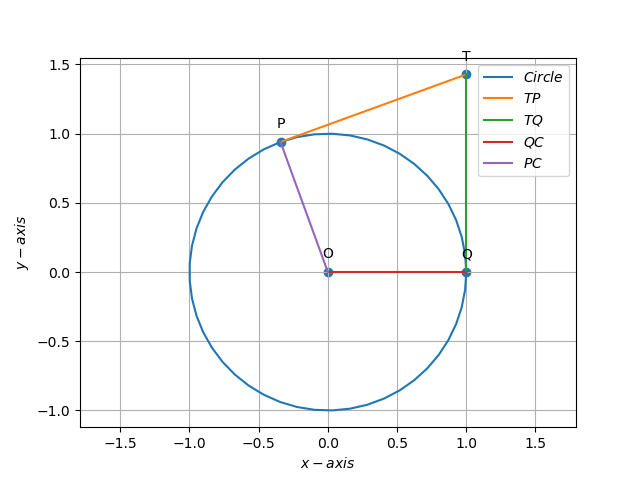
\includegraphics[width=\columnwidth]{chapters/10/10/2/2/figs/tangent2}
	\end{center}
\caption{}
\label{fig:chapters/10/10/2/2/Fig1}
\end{figure}



















\item If the tangents $PA$ and $PB$ from a point $\vec{P}$ to a circle with center $\vec{O}$ are inclined to each other at $80{\degree}$, find $\angle{POA}$.
\\
\solution
\iffalse
\documentclass[journal,12pt,twocolumn]{IEEEtran}
%
\usepackage{setspace}
\usepackage{gensymb}
%\doublespacing
\singlespacing

%\usepackage{graphicx}
%\usepackage{amssymb}
%\usepackage{relsize}
\usepackage[cmex10]{amsmath}
%\usepackage{amsthm}
%\interdisplaylinepenalty=2500
%\savesymbol{iint}
%\usepackage{txfonts}
%\restoresymbol{TXF}{iint}
%\usepackage{wasysym}
\usepackage{amsthm}
%\usepackage{iithtlc}
\usepackage{mathrsfs}
\usepackage{txfonts}
\usepackage{stfloats}
\usepackage{bm}
\usepackage{cite}
\usepackage{cases}
\usepackage{subfig}
%\usepackage{xtab}
\usepackage{longtable}
\usepackage{multirow}
%\usepackage{algorithm}
%\usepackage{algpseudocode}
\usepackage{enumitem}
\usepackage{mathtools}
\usepackage{steinmetz}
\usepackage{tikz}
\usepackage{circuitikz}
\usepackage{verbatim}
\usepackage{tfrupee}
\usepackage[breaklinks=true]{hyperref}
%\usepackage{stmaryrd}
\usepackage{tkz-euclide} % loads  TikZ and tkz-base
%\usetkzobj{all}
\usetikzlibrary{calc,math}
\usepackage{listings}
    \usepackage{color}                                            %%
    \usepackage{array}                                            %%
    \usepackage{longtable}                                        %%
    \usepackage{calc}                                             %%
    \usepackage{multirow}                                         %%
    \usepackage{hhline}                                           %%
    \usepackage{ifthen}                                           %%
  %optionally (for landscape tables embedded in another document): %%
    \usepackage{lscape}     
\usepackage{multicol}
\usepackage{chngcntr}
%\usepackage{enumerate}

%\usepackage{wasysym}
%\newcounter{MYtempeqncnt}
\DeclareMathOperator*{\Res}{Res}
%\renewcommand{\baselinestretch}{2}
\renewcommand\thesection{\arabic{section}}
\renewcommand\thesubsection{\thesection.\arabic{subsection}}
\renewcommand\thesubsubsection{\thesubsection.\arabic{subsubsection}}

\renewcommand\thesectiondis{\arabic{section}}
\renewcommand\thesubsectiondis{\thesectiondis.\arabic{subsection}}
\renewcommand\thesubsubsectiondis{\thesubsectiondis.\arabic{subsubsection}}

% correct bad hyphenation here
\hyphenation{op-tical net-works semi-conduc-tor}
\def\inputGnumericTable{}                                 %%

\lstset{
%language=C,
frame=single, 
breaklines=true,
columns=fullflexible
}
%\lstset{
%language=tex,
%frame=single, 
%breaklines=true
%}

\begin{document}
%


\newtheorem{theorem}{Theorem}[section]
\newtheorem{problem}{Problem}
\newtheorem{proposition}{Proposition}[section]
\newtheorem{lemma}{Lemma}[section]
\newtheorem{corollary}[theorem]{Corollary}
\newtheorem{example}{Example}[section]
\newtheorem{definition}[problem]{Definition}
%\newtheorem{thm}{Theorem}[section] 
%\newtheorem{defn}[thm]{Definition}
%\newtheorem{algorithm}{Algorithm}[section]
%\newtheorem{cor}{Corollary}
\newcommand{\BEQA}{\begin{eqnarray}}
\newcommand{\EEQA}{\end{eqnarray}}
\newcommand{\define}{\stackrel{\triangle}{=}}

\bibliographystyle{IEEEtran}
%\bibliographystyle{ieeetr}


\providecommand{\mbf}{\mathbf}
\providecommand{\pr}[1]{\ensuremath{\Pr\left(#1\right)}}
\providecommand{\qfunc}[1]{\ensuremath{Q\left(#1\right)}}
\providecommand{\sbrak}[1]{\ensuremath{{}\left[#1\right]}}
\providecommand{\lsbrak}[1]{\ensuremath{{}\left[#1\right.}}
\providecommand{\rsbrak}[1]{\ensuremath{{}\left.#1\right]}}
\providecommand{\brak}[1]{\ensuremath{\left(#1\right)}}
\providecommand{\lbrak}[1]{\ensuremath{\left(#1\right.}}
\providecommand{\rbrak}[1]{\ensuremath{\left.#1\right)}}
\providecommand{\cbrak}[1]{\ensuremath{\left\{#1\right\}}}
\providecommand{\lcbrak}[1]{\ensuremath{\left\{#1\right.}}
\providecommand{\rcbrak}[1]{\ensuremath{\left.#1\right\}}}
\theoremstyle{remark}
\newtheorem{rem}{Remark}
\newcommand{\sgn}{\mathop{\mathrm{sgn}}}
\providecommand{\abs}[1]{\left\vert#1\right\vert}
\providecommand{\res}[1]{\Res\displaylimits_{#1}} 
\providecommand{\norm}[1]{\left\lVert#1\right\rVert}
%\providecommand{\norm}[1]{\lVert#1\rVert}
\providecommand{\mtx}[1]{\mathbf{#1}}
\providecommand{\mean}[1]{E\left[ #1 \right]}
\providecommand{\fourier}{\overset{\mathcal{F}}{ \rightleftharpoons}}
%\providecommand{\hilbert}{\overset{\mathcal{H}}{ \rightleftharpoons}}
\providecommand{\system}{\overset{\mathcal{H}}{ \longleftrightarrow}}
	%\newcommand{\solution}[2]{\textbf{Solution:}{#1}}
\newcommand{\solution}{\noindent \textbf{Solution: }}
\newcommand{\cosec}{\,\text{cosec}\,}
\providecommand{\dec}[2]{\ensuremath{\overset{#1}{\underset{#2}{\gtrless}}}}
\newcommand{\myvec}[1]{\ensuremath{\begin{pmatrix}#1\end{pmatrix}}}
\newcommand{\mydet}[1]{\ensuremath{\begin{vmatrix}#1\end{vmatrix}}}
%\numberwithin{equation}{section}
\numberwithin{equation}{subsection}
%\numberwithin{problem}{section}
%\numberwithin{definition}{section}
\makeatletter
\@addtoreset{figure}{problem}
\makeatother

\let\StandardTheFigure\thefigure
\let\vec\mathbf
%\renewcommand{\thefigure}{\theproblem.\arabic{figure}}
\renewcommand{\thefigure}{\theproblem}
%\setlist[enumerate,1]{before=\renewcommand\theequation{\theenumi.\arabic{equation}}
%\counterwithin{equation}{enumi}


%\renewcommand{\theequation}{\arabic{subsection}.\arabic{equation}}

\def\putbox#1#2#3{\makebox[0in][l]{\makebox[#1][l]{}\raisebox{\baselineskip}[0in][0in]{\raisebox{#2}[0in][0in]{#3}}}}
     \def\rightbox#1{\makebox[0in][r]{#1}}
     \def\centbox#1{\makebox[0in]{#1}}
     \def\topbox#1{\raisebox{-\baselineskip}[0in][0in]{#1}}
     \def\midbox#1{\raisebox{-0.5\baselineskip}[0in][0in]{#1}}

\vspace{3cm}


\title{Problem: 10.10.2.3}
\author{Nikam Pratik Balasaheb (EE21BTECH11037)}





% make the title area
\maketitle

\newpage

%\tableofcontents

\bigskip

\renewcommand{\thefigure}{\theenumi}
\renewcommand{\thetable}{\theenumi}
%\renewcommand{\theequation}{\theenumi}

\section{Problem}
\section{Solution}
\fi
The input parameters are listed in Table 
\ref{tab:chapters/10/10/2/3/}.
Since
\begin{align}
	\angle{APB} &= 80{\degree}\\
	\angle{APO} &= \frac{1}{2} \angle{APB}\\
		    &= 40 \degree\;\; = \theta\; (say)
\end{align}
Therefore, it can be said that $\vec{P}$ lies on the line
\begin{align}
	\myvec{-\sin{\theta} & \cos{\theta}} \vec{x} =0
\end{align}
Let the circle be $\norm{\vec{x}}^2 = r^2$ and $\vec{A}$ be $\myvec{0\\r}$.
Therefore, the tangent that P lies on is given by
\begin{align}
	\myvec{0 & 1} \vec{x} = r
\end{align}
The point $\vec{P}$ is given by:
\begin{align}
	\myvec{ -\cos{\theta} & \sin{\theta} \\ 0 &1} \vec{x} = \myvec{0\\r}
\end{align}
The augmented matrix for the above equation is 
\begin{align}
	\myvec{ -\sin{\theta} & \cos{\theta} &\vrule & 0 \\
	0 & 1 & \vrule & r}\\
	\xleftrightarrow{R_1 \leftarrow \frac{R_1}{-\sin{\theta}} + \cot{\theta} R_2}\\
	\myvec{ 1 & 0 & \vrule & r\cot{\theta}\\
	0 & 1 & \vrule & r}
\end{align}
yielding
\begin{align}
	\vec{P} = \myvec{r \cot{\theta} \\ r}
\end{align}
Let $\angle{POA} = \phi$.  Then, 
\begin{align}
	\cos{\phi} &= \frac{ \brak{\vec{P}-\vec{O}}^{\top} \brak{\vec{A}-\vec{O}} }{ \norm{\vec{P}-\vec{O}} \norm{\vec{A}-\vec{O}}}\\ 
		   &= \frac{ \myvec{r \cot{\theta} & r} \myvec{ 0\\r} }{ r^2 \cosec{\theta} }\\
	\cos{\phi} &= \sin{\theta}\\
	\implies \; \phi &= 90\degree - \theta\\
	\phi &= 50 \degree
\end{align}
\begin{table}[h!]
\begin{center}
	%%%%%%%%%%%%%%%%%%%%%%%%%%%%%%%%%%%%%%%%%%%%%%%%%%%%%%%%%%%%%%%%%%%%%%
%%                                                                  %%
%%  This is a LaTeX2e table fragment exported from Gnumeric.        %%
%%                                                                  %%
%%%%%%%%%%%%%%%%%%%%%%%%%%%%%%%%%%%%%%%%%%%%%%%%%%%%%%%%%%%%%%%%%%%%%%

\begin{tabular}[]{|c|c|c|}
\hline
$\vec{O}$	& $\myvec{0\\0}$ &Center of the given circle \\ \hline
$\vec{A}$	& $\myvec{0\\5}$ &Point where tangent is taken\\ \hline
$r$		& 5 & radius of given circle \\ \hline
$\angle{APB}$ 		& $80\degree$ & Angle between tangents\\ \hline
\end{tabular}

\end{center}
\caption{Table 1}
\label{tab:chapters/10/10/2/3/}
\end{table}
See Fig. 
    \ref{fig:chapters/10/10/2/3/}.
\begin{figure}[h!]
  \centering
    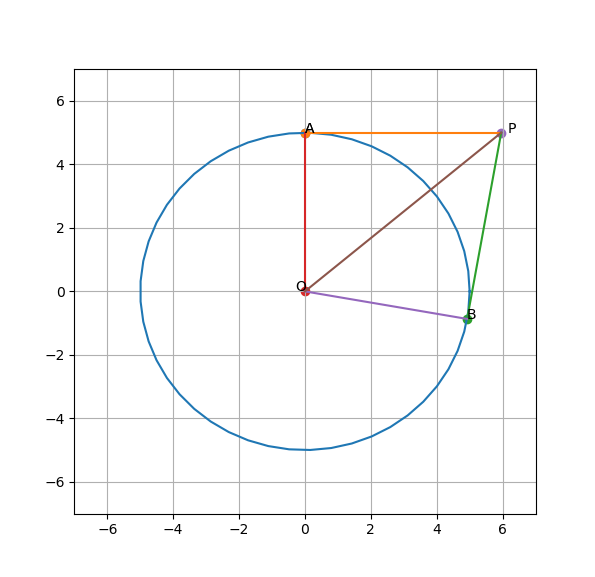
\includegraphics[width=\columnwidth,height=\columnwidth]{chapters/10/10/2/3/figs/Figure_1.png}
    \caption{Figure 1}
    \label{fig:chapters/10/10/2/3/}
\end{figure}





\item 
\label{chapters/10/10/2/4}
\iffalse
\documentclass[journal,12pt,twocolumn]{article}
\usepackage{graphicx}
\usepackage[none]{hyphenat}
\usepackage[margin=0.5in]{geometry}
\usepackage[cmex10]{amsmath}
\usepackage{array}
\usepackage{booktabs}
\usepackage{gensymb}
\usepackage{textcomp}
\title{\textbf{Circle Assignment}}
\author{Manideep Parusha - FWC22004}
\date{\today}

\providecommand{\norm}[1]{\left\lVert#1\right\rVert}
\providecommand{\abs}[1]{\left\vert#1\right\vert}
\let\vec\mathbf
\newcommand{\myvec}[1]{\ensuremath{\begin{pmatrix}#1\end{pmatrix}}}
\newcommand{\mydet}[1]{\ensuremath{\begin{vmatrix}#1\end{vmatrix}}}
\providecommand{\brak}[1]{\ensuremath{\left(#1\right)}}

\begin{document}

\maketitle
\section*{Problem}
\paragraph{
\fi
	Show that the tangents of circle drawn at the ends of diameter are parallel.
	\begin{figure}[!ht]
		\centering
 \includegraphics[width=\columnwidth]{chapters/10/10/2/4/figs/plot_cir.png}
		\caption{}
		\label{fig:10/10/2/4}
  	\end{figure}
	\\
	\solution See Fig. 
		\ref{fig:10/10/2/4}.
	\iffalse
\section*{Solution}

\begin{figure}[h]
\centering
\includegraphics[width=\columnwidth]{figs/plot_cir.png}
\caption{Circle with tangents at ends of it's diameter}
\label{fig:cir_py}
\end{figure}

\subsection*{Construction}
Input taken for the construction of the Circle and the tangents is 'r' radius of the circle.

\begin{table}[h]
	\centering
\setlength\extrarowheight{2pt}
	\begin{tabular}{|c|c|c|}
		\hline
		\textbf{Symbol} & \textbf{Value} & \textbf{Description} \\
		\hline
		r & 10 & circle radius\\
		\hline
		O & $-\vec{u}$ & Center\\
		\hline
		A & \myvec{a_1\\a_2} & point A\\
		\hline
		B & \myvec{b_1\\b_2} & point B\\
		\hline
	\end{tabular}
\end{table}

Let us assume a circle with radius 'r' and center at origin.\\
\begin{align}
	\vec{x}^{T}\vec{Vx} + 2\vec{u}^{T}\vec{x} + f = 0
\end{align}
but, for a Circle 
\begin{align}
	\vec{V} = \myvec{ 1 & 0 \\0 & 1}
\end{align}
and the center of the circle is,
\begin{align}
	-\vec{u} = \myvec{u_1 \\ u_2}
	\label{center}
\end{align}
\fi
Let $\vec{A}, \vec{B}$ be  the end points of the diameter of the circle through which the tangents are drawn.
From 
	\eqref{eq:circ-cr},
\begin{align}
	\frac{\vec{A} + \vec{B}}{2} = -\vec{u} \\
	\implies \vec{A}+\vec{B} = -2\vec{u}
	\label{ab}
\end{align}

From 
  \eqref{eq:conic_tangent_mq},
  \begin{align}
	  \vec{m}_1^{\top}\brak{\vec{A}+\vec{u}} &= 0
	  \\
	  \vec{m}_2^{\top}\brak{\vec{B}+\vec{u}} &= 0
  \end{align}
where $\vec{m_1}, \vec{m_2}$ are the direction vectors of the tangents at $\vec{A}, \vec{B}$ respectively.
Then, the normal vectors at the point of contact of tangets are
\begin{align}
	\vec{A}+\vec{u} &= k_1\vec{n_1}
	\label{n1}
	\\
	\vec{B}+\vec{u} &= k_2\vec{n_2}
	\label{n2}
\end{align}
Adding \eqref{n1} and \eqref{n2}, 
\begin{align}
	k_1\vec{n_1}+k_2\vec{n_2} &=\vec{A}+\vec{B} + 2\vec{u}  
	\\
	&=\vec{0}
	\label{addeq}
\end{align}
from \eqref{ab}, \eqref{addeq} can be expressed as 
 \begin{align}
	 k_1\vec{n_1}+k_2\vec{n_2} &= 0 \\
	 k_1\vec{n_1} &= -k_2\vec{n_2}
 \end{align}
Since 
\begin{align}
	\vec{n_1} \times \vec{n_2} &= \vec{0},
	\\
	\vec{n_1} \parallel \vec{n_2}  &\implies 
	\vec{m_1} \parallel \vec{m_2}  
\end{align}
\iffalse

 So the tangents are parallel to each other.\\
Hence, we have proved that the tangents at the ends of the diameter of a circle are parallel.
\end{document}
\fi

\item 
\label{chapters/10/10/2/5}
%\iffalse
\documentclass[12pt]{article}
\usepackage{graphicx}
\usepackage{amsmath}
\usepackage{mathtools}
\usepackage{gensymb}
\usepackage{amssymb}
\usepackage{tikz}
\usetikzlibrary{arrows,shapes,automata,petri,positioning,calc}
\usepackage{hyperref}
\usepackage{tikz}
\usetikzlibrary{matrix,calc}
\usepackage[margin=0.5in]{geometry}

\providecommand{\norm}[1]{\left\lVert#1\right\rVert}
\newcommand{\myvec}[1]{\ensuremath{\begin{pmatrix}#1\end{pmatrix}}}
\let\vec\mathbf
%\providecommand $${\norm}[1]{\left\lVert#1\right\rVert}$$
\providecommand{\abs}[1]{\left\vert#1\right\vert}
\let\vec\mathbf

\newcommand{\mydet}[1]{\ensuremath{\begin{vmatrix}#1\end{vmatrix}}}
\providecommand{\brak}[1]{\ensuremath{\left(#1\right)}}
\providecommand{\lbrak}[1]{\ensuremath{\left(#1\right.}}
\providecommand{\rbrak}[1]{\ensuremath{\left.#1\right)}}
\providecommand{\sbrak}[1]{\ensuremath{{}\left[#1\right]}}

\providecommand{\brak}[1]{\ensuremath{\left(#1\right)}}
\providecommand{\norm}[1]{\left\lVert#1\right\rVert}
\newcommand{\solution}{\noindent \textbf{Solution: }}

\let\vec\mathbf
\def\inputGnumericTable{}
\usepackage{color}                                            %%
    \usepackage{array}                                            %%
    \usepackage{longtable}                                        %%
    \usepackage{calc}                                             %%
    \usepackage{multirow}                                         %%
    \usepackage{hhline}                                           %%
    \usepackage{ifthen}
\usepackage{array}
\usepackage{amsmath}   % for having text in math mode
\usepackage{listings}
\lstset{
language=tex,
frame=single, 
breaklines=true
}
\newenvironment{Figure}
  {\par\medskip\noindent\minipage{\linewidth}}
  {\endminipage\par\medskip}
\begin{document}
\begin{center}
\textbf\large{CLASS-9\\CHAPTER-10 \\ CIRCLES}

\end{center}
\section*{Excercise 10.6}

\section*{\large Solution}:
\fi
The input parameters are available in Table 
	\ref{tab:chapters/9/10/6/1/table1}.
\begin{figure}[h!]
\centering
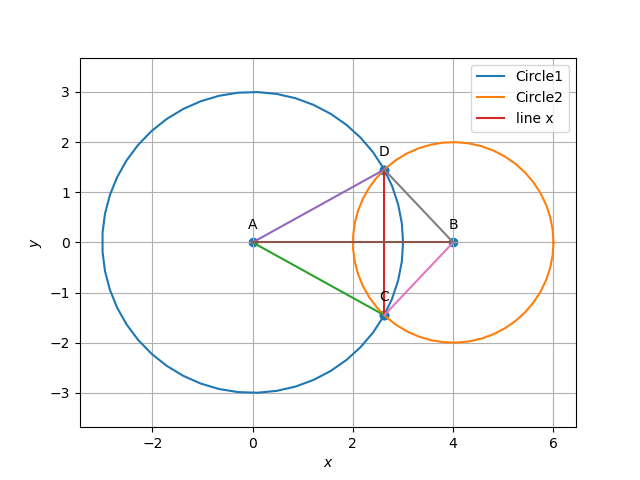
\includegraphics[width=\columnwidth]{chapters/9/10/6/1/figs/circle3.png}
\caption{}
\label{fig:chapters/9/10/6/1/Fig1}
\end{figure}



\begin{table}[h!]
	\small
	\centering
	%\subimport{../chapters/9/10/6/1/tables/}{table1.tex}
     %%%%%%%%%%%%%%%%%%%%%%%%%%%%%%%%%%%%%%%%%%%%%%%%%%%%%%%%%%%%%%%%%%%%%%
%%                                                                  %%
%%  This is the header of a LaTeX2e file exported from Gnumeric.    %%
%%                                                                  %%
%%  This file can be compiled as it stands or included in another   %%
%%  LaTeX document. The table is based on the longtable package so  %%
%%  the longtable options (headers, footers...) can be set in the   %%
%%  preamble section below (see PRAMBLE).                           %%
%%                                                                  %%
%%  To include the file in another, the following two lines must be %%
%%  in the including file:                                          %%
%%        \def\inputGnumericTable{}                                 %%
%%  at the beginning of the file and:                               %%
%%        \input{name-of-this-file.tex}                             %%
%%  where the table is to be placed. Note also that the including   %%
%%  file must use the following packages for the table to be        %%
%%  rendered correctly:                                             %%
%%    \usepackage[latin1]{inputenc}                                 %%
%%    \usepackage{color}                                            %%
%%    \usepackage{array}                                            %%
%%    \usepackage{longtable}                                        %%
%%    \usepackage{calc}                                             %%
%%    \usepackage{multirow}                                         %%
%%    \usepackage{hhline}                                           %%
%%    \usepackage{ifthen}                                           %%
%%  optionally (for landscape tables embedded in another document): %%
%%    \usepackage{lscape}                                           %%
%%                                                                  %%
%%%%%%%%%%%%%%%%%%%%%%%%%%%%%%%%%%%%%%%%%%%%%%%%%%%%%%%%%%%%%%%%%%%%%



%%  This section checks if we are begin input into another file or  %%
%%  the file will be compiled alone. First use a macro taken from   %%
%%  the TeXbook ex 7.7 (suggestion of Han-Wen Nienhuys).            %%
\def\ifundefined#1{\expandafter\ifx\csname#1\endcsname\relax}


%%  Check for the \def token for inputed files. If it is not        %%
%%  defined, the file will be processed as a standalone and the     %%
%%  preamble will be used.                                          %%
\ifundefined{inputGnumericTable}

%%  We must be able to close or not the document at the end.        %%
	\def\gnumericTableEnd{\end{document}}


%%%%%%%%%%%%%%%%%%%%%%%%%%%%%%%%%%%%%%%%%%%%%%%%%%%%%%%%%%%%%%%%%%%%%%
%%                                                                  %%
%%  This is the PREAMBLE. Change these values to get the right      %%
%%  paper size and other niceties.                                  %%
%%                                                                  %%
%%%%%%%%%%%%%%%%%%%%%%%%%%%%%%%%%%%%%%%%%%%%%%%%%%%%%%%%%%%%%%%%%%%%%%

	\documentclass[12pt%
			  %,landscape%
                    ]{report}
       \usepackage[latin1]{inputenc}
       \usepackage{fullpage}
       \usepackage{color}
       \usepackage{array}
       \usepackage{longtable}
       \usepackage{calc}
       \usepackage{multirow}
       \usepackage{hhline}
       \usepackage{ifthen}
       \usepackage{gensymb}
       \usepackage{graphicx}
\usepackage{amsmath}
\usepackage{mathtools}
\newcommand{\mydet}[1]{\ensuremath{\begin{vmatrix}#1\end{vmatrix}}}
\providecommand{\brak}[1]{\ensuremath{\left(#1\right)}}
\providecommand{\norm}[1]{\left\lVert#1\right\rVert}
\newcommand{\solution}{\noindent \textbf{Solution: }}
\newcommand{\myvec}[1]{\ensuremath{\begin{pmatrix}#1\end{pmatrix}}}
\let\vec\mathbf
	\begin{document}


%%  End of the preamble for the standalone. The next section is for %%
%%  documents which are included into other LaTeX2e files.          %%
\else

%%  We are not a stand alone document. For a regular able, we will %%
%%  have no preamble and only define the closing to mean nothing.   %%
    \def\gnumericTableEnd{}

%%  If we want landscape mode in an embedded document, comment out  %%
%%  the line above and uncomment the two below. The table will      %%
%%  begin on a new page and run in landscape mode.                  %%
%       \def\gnumericTableEnd{\end{landscape}}
%       \begin{landscape}


%%  End of the else clause for this file being \input.              %%
\fi

%%%%%%%%%%%%%%%%%%%%%%%%%%%%%%%%%%%%%%%%%%%%%%%%%%%%%%%%%%%%%%%%%%%%%%
%%                                                                  %%
%%  The rest is the gnumeric table, except for the closing          %%
%%  statement. Changes below will alter the table's appearance.     %%
%%                                                                  %%
%%%%%%%%%%%%%%%%%%%%%%%%%%%%%%%%%%%%%%%%%%%%%%%%%%%%%%%%%%%%%%%%%%%%%%
\providecommand{\gnumericmathit}[1]{#1} 
%%  Uncomment the next line if you would like your numbers to be in %%
%%  italics if they are italizised in the gnumeric table.           %%
%\renewcommand{\gnumericmathit}[1]{\mathit{#1}}
\providecommand{\gnumericPB}[1]%
{\let\gnumericTemp=\\#1\let\\=\gnumericTemp\hspace{0pt}}
 \ifundefined{gnumericTableWidthDefined}
        \newlength{\gnumericTableWidth}
        \newlength{\gnumericTableWidthComplete}
        \newlength{\gnumericMultiRowLength}
        \global\def\gnumericTableWidthDefined{}
 \fi
%% The following setting protects this code from babel shorthands.  %%
 \ifthenelse{\isundefined{\languageshorthands}}{}{\languageshorthands{english}}
%%  The default table format retains the relative column widths of  %%
%%  gnumeric. They can easily be changed to c, r or l. In that case %%
%%  you may want to comment out the next line and uncomment the one %%
%%  thereafter                                                      %%
\providecommand\gnumbox{\makebox[0pt]}
%%\providecommand\gnumbox[1][]{\makebox}

%% to adjust positions in multirow situations                       %%
\setlength{\bigstrutjot}{\jot}
\setlength{\extrarowheight}{\doublerulesep}

%%  The \setlongtables command keeps column widths the same across  %%
%%  pages. Simply comment out next line for varying column widths.  %%
\setlongtables

\setlength\gnumericTableWidth{%
	40pt+%
	35pt+%
	210pt+%
0pt}
\def\gumericNumCols{3}
\setlength\gnumericTableWidthComplete{\gnumericTableWidth+%
         \tabcolsep*\gumericNumCols*2+\arrayrulewidth*\gumericNumCols}
\ifthenelse{\lengthtest{\gnumericTableWidthComplete > \linewidth}}%
         {\def\gnumericScale{\ratio{\linewidth-%
                        \tabcolsep*\gumericNumCols*2-%
                        \arrayrulewidth*\gumericNumCols}%
{\gnumericTableWidth}}}%
{\def\gnumericScale{1}}

%%%%%%%%%%%%%%%%%%%%%%%%%%%%%%%%%%%%%%%%%%%%%%%%%%%%%%%%%%%%%%%%%%%%%%
%%                                                                  %%
%% The following are the widths of the various columns. We are      %%
%% defining them here because then they are easier to change.       %%
%% Depending on the cell formats we may use them more than once.    %%
%%                                                                  %%
%%%%%%%%%%%%%%%%%%%%%%%%%%%%%%%%%%%%%%%%%%%%%%%%%%%%%%%%%%%%%%%%%%%%%%

\ifthenelse{\isundefined{\gnumericColA}}{\newlength{\gnumericColA}}{}\settowidth{\gnumericColA}{\begin{tabular}{@{}p{40pt*\gnumericScale}@{}}x\end{tabular}}
\ifthenelse{\isundefined{\gnumericColB}}{\newlength{\gnumericColB}}{}\settowidth{\gnumericColB}{\begin{tabular}{@{}p{35pt*\gnumericScale}@{}}x\end{tabular}}
\ifthenelse{\isundefined{\gnumericColC}}{\newlength{\gnumericColC}}{}\settowidth{\gnumericColC}{\begin{tabular}{@{}p{210pt*\gnumericScale}@{}}x\end{tabular}}

\begin{longtable}[c]{%
	b{\gnumericColA}%
	b{\gnumericColB}%
	b{\gnumericColC}%
	}

%%%%%%%%%%%%%%%%%%%%%%%%%%%%%%%%%%%%%%%%%%%%%%%%%%%%%%%%%%%%%%%%%%%%%%
%%  The longtable options. (Caption, headers... see Goosens, p.124) %%
%	\caption{The Table Caption.}             \\	%
% \hline	% Across the top of the table.
%%  The rest of these options are table rows which are placed on    %%
%%  the first, last or every page. Use \multicolumn if you want.    %%

%%  Header for the first page.                                      %%
%	\multicolumn{3}{c}{The First Header} \\ \hline 
%	\multicolumn{1}{c}{colTag}	%Column 1
%	&\multicolumn{1}{c}{colTag}	%Column 2
%	&\multicolumn{1}{c}{colTag}	\\ \hline %Last column
%	\endfirsthead

%%  The running header definition.                                  %%
%	\hline
%	\multicolumn{3}{l}{\ldots\small\slshape continued} \\ \hline
%	\multicolumn{1}{c}{colTag}	%Column 1
%	&\multicolumn{1}{c}{colTag}	%Column 2
%	&\multicolumn{1}{c}{colTag}	\\ \hline %Last column
%	\endhead

%%  The running footer definition.                                  %%
%	\hline
%	\multicolumn{3}{r}{\small\slshape continued\ldots} \\
%	\endfoot

%%  The ending footer definition.                                   %%
%	\multicolumn{3}{c}{That's all folks} \\ \hline 
%	\endlastfoot
%%%%%%%%%%%%%%%%%%%%%%%%%%%%%%%%%%%%%%%%%%%%%%%%%%%%%%%%%%%%%%%%%%%%%%

\hhline{|-|-|-}
	 \multicolumn{1}{|p{\gnumericColA}|}%
	{\gnumericPB{\raggedright}\gnumbox[l]{\textbf{Symbol}}}
	&\multicolumn{1}{p{\gnumericColB}|}%
	{\gnumericPB{\raggedright}\gnumbox[l]{\textbf{Values}}}
	&\multicolumn{1}{p{\gnumericColC}|}%
	{\gnumericPB{\raggedright}\gnumbox[l]{\textbf{Description}}}
\\
\hhline{|---|}
	 \multicolumn{1}{|p{\gnumericColA}|}%
	{\gnumericPB{\raggedright}\gnumbox[l]{$\vec{A}$}}
	&\multicolumn{1}{p{\gnumericColB}|}%
	{\gnumericPB{\raggedright}\gnumbox[l]{\myvec{0\\0}}}
	&\multicolumn{1}{p{\gnumericColC}|}%
	{\gnumericPB{\raggedright}\gnumbox[l]{Center of circle 1}}
\\
\hhline{|---|}
	 \multicolumn{1}{|p{\gnumericColA}|}%
	{\gnumericPB{\raggedright}\gnumbox[l]{$r_1$}}
	&\multicolumn{1}{p{\gnumericColB}|}%
	{\gnumericPB{\raggedright}\gnumbox[l]{3 units}}
	&\multicolumn{1}{p{\gnumericColC}|}%
	{\gnumericPB{\raggedright}\gnumbox[l]{Radius of the circle 1 }}
\\
\hhline{|---|}
	 \multicolumn{1}{|p{\gnumericColA}|}%
	{\gnumericPB{\raggedright}\gnumbox[l]{$\vec{B}$}}
	&\multicolumn{1}{p{\gnumericColB}|}%
	{\gnumericPB{\raggedright}\gnumbox[l]{\myvec{4\\0}}}
	&\multicolumn{1}{p{\gnumericColC}|}%
	{\gnumericPB{\raggedright}\gnumbox[l]{Center of circle 2}}
\\
\hhline{|---|}
	 \multicolumn{1}{|p{\gnumericColA}|}%
	{\gnumericPB{\raggedright}\gnumbox[l]{$r_2$}}
	&\multicolumn{1}{p{\gnumericColB}|}%
	{\gnumericPB{\raggedright}\gnumbox[l]{2 units}}
	&\multicolumn{1}{p{\gnumericColC}|}%
	{\gnumericPB{\raggedright}\gnumbox[l]{Radius of circle 2}}
\\
\hhline{|---|}
	 \multicolumn{1}{|p{\gnumericColA}|}%
	{\gnumericPB{\raggedright}\gnumbox[l]{$\vec{e}_1$}}
	&\multicolumn{1}{p{\gnumericColB}|}%
	{\gnumericPB{\raggedright}\gnumbox[l]{\myvec{1\\0}}}
	&\multicolumn{1}{p{\gnumericColC}|}%
	{\gnumericPB{\raggedright}\gnumbox[l]{Standard basis vector 1}}
\\
\hhline{|---|}
\multicolumn{1}{|p{\gnumericColA}|}%
	{\gnumericPB{\raggedright}\gnumbox[l]{$\vec{e}_2$}}
	&\multicolumn{1}{p{\gnumericColB}|}%
	{\gnumericPB{\raggedright}\gnumbox[l]{\myvec{0\\1}}}
	&\multicolumn{1}{p{\gnumericColC}|}%
	{\gnumericPB{\raggedright}\gnumbox[l]{Standard basis vector 2}}
	\\
\hhline{|---|}
\end{longtable}

\ifthenelse{\isundefined{\languageshorthands}}{}{\languageshorthands{\languagename}}
\gnumericTableEnd%t
%	\caption{}
	\label{tab:chapters/9/10/6/1/table1}
\end{table}
 The two circle equations are given by
\begin{align}
\label{eq:chapters/9/10/6/1/1}
	\norm{x}^2-9&=0\\
	\norm{x}^2-8\vec{e}_1+12&=0
\end{align}
yielding the intersection of the circles as the line
\begin{align}
\myvec{1&0}\vec{x}&=\frac{21}{8}\\
\label{eq:chapters/9/10/6/1/20}
\end{align}
		\eqref{eq:chapters/9/10/6/1/20} can be expressed as
\begin{align}
	\vec{x}=\vec{q}+\lambda\vec{m}\label{eq:chapters/9/10/6/1/21}
\end{align}
The distance form origin to point $\vec{x}$ is given by
\begin{align}
	\norm{\vec{x}}^2&=d^2\label{eq:chapters/9/10/6/1/22}
\end{align}
		Then substituting \eqref{eq:chapters/9/10/6/1/21} in \eqref{eq:chapters/9/10/6/1/22} yeilds,
\begin{align}
	\brak{\vec{q}+\lambda\vec{m}}^{\top}\brak{\vec{q}+\lambda\vec{m}}&=d^2\\
	\implies \lambda^2\norm{\vec{m}}^2+2\lambda\vec{q}^{\top}\vec{m}+\norm{\vec{q}}^2&=d^2\label{eq:chapters/9/10/6/1/26}
\end{align}
where
\begin{align}
	\vec{q}=\myvec{\frac{21}{8}\\0},\vec{m}=\myvec{0\\1} \text{ and } d=r_1=3
	\label{eq:chapters/9/10/6/1/27}
\end{align}
		Substituting the values in \eqref{eq:chapters/9/10/6/1/27} in \eqref{eq:chapters/9/10/6/1/26}, 
\begin{align}
	\lambda^2(1)+2\lambda\myvec{\frac{21}{8}&0}\myvec{0\\1}+\frac{441}{64}&=9\\
	\implies\lambda_i&=\pm\frac{3\sqrt{5}}{8}
\end{align}
Thus, 
the intersecting points $\vec{C}$ and $\vec{D}$ are given by
\begin{align}
    \vec{C}&=\vec{q}+\lambda_1\vec{m}=\myvec{\frac{21}{8}\\[2pt]-\frac{3\sqrt{5}}{8}}\\
    \vec{D}&=\vec{q}+\lambda_2\vec{m}=\myvec{\frac{21}{8}\\[2pt]\frac{3\sqrt{5}}{8}}
\end{align}
\begin{enumerate}
\item Finding $\angle$ADB
	\begin{align}
		 \vec{A-D} = \myvec{-\frac{21}{8}\\[2pt]-\frac{3\sqrt{5}}{8}},
		\vec{B-D}& = \myvec{\frac{11}{8}\\[2pt]-\frac{3\sqrt{5}}{8}}\\
	 \vec{(A-D)^\top(B-D)}&= -\frac{3}{2}\\
	 \norm{\vec{A-D}}\norm{\vec{C-D}}& = 6\\
\implies		\cos(\angle ADB)& = \frac{\vec{(A-D)^\top(B-D)}}{\norm{\vec{A-D}}\norm{\vec{B-D}}}\\
		\text{or, }		\angle ADB&=104\degree
\end{align}
\item Finding $\angle$ACB
\begin{align}
	\vec{A-C} = \myvec{-\frac{21}{8}\\[2pt]\frac{3\sqrt{5}}{8}},
	 \vec{B-C}& = \myvec{\frac{11}{8}\\[2pt]\frac{3\sqrt{5}}{8}}\\
	 \vec{(A-C)^\top(B-C)}&= -\frac{3}{2}\\
	 \norm{\vec{A-C}}\norm{\vec{B-C}}& = 6\\
\implies 	 \cos(\angle ACB) &= \frac{\vec{(A-C)^\top(B-C)}}{\norm{\vec{A-C}}\norm{\vec{B-C}}}\\
	\text{or, }	 \angle ACB&=104\degree = \angle ADB
\end{align}
\end{enumerate}
See Fig. 
\ref{fig:chapters/9/10/6/1/Fig1}.



\item 
\label{chapters/10/10/2/6}
\iffalse
\documentclass[journal,10pt,twocolumn]{article}
\usepackage{graphicx}
\usepackage[margin=0.5in]{geometry}
\usepackage{amsmath}
\usepackage{array}
\usepackage{booktabs}
\usepackage{enumerate}
\providecommand{\norm}[1]{\left\lVert#1\right\rVert}
\providecommand{\abs}[1]{\left\vert#1\right\vert}
\let\vec\mathbf
\newcommand{\myvec}[1]{\ensuremath{\begin{pmatrix}#1\end{pmatrix}}}
\newcommand{\mydet}[1]{\ensuremath{\begin{vmatrix}#1\end{vmatrix}}}
\providecommand{\brak}[1]{\ensuremath{\left(#1\right)}}
\title{\textbf{Matrix Assignment}}
\author{Mannava Venkatasai}
\date{September 2022}

\begin{document}

\maketitle
\paragraph{\textit{Problem Statement} -
\fi
The length of a tangent from a point $\vec{A}$ at distance 5 cm from the centre of the circle is 4
cm. Find the radius of the circle.
	\begin{figure}[!h]
		\centering
 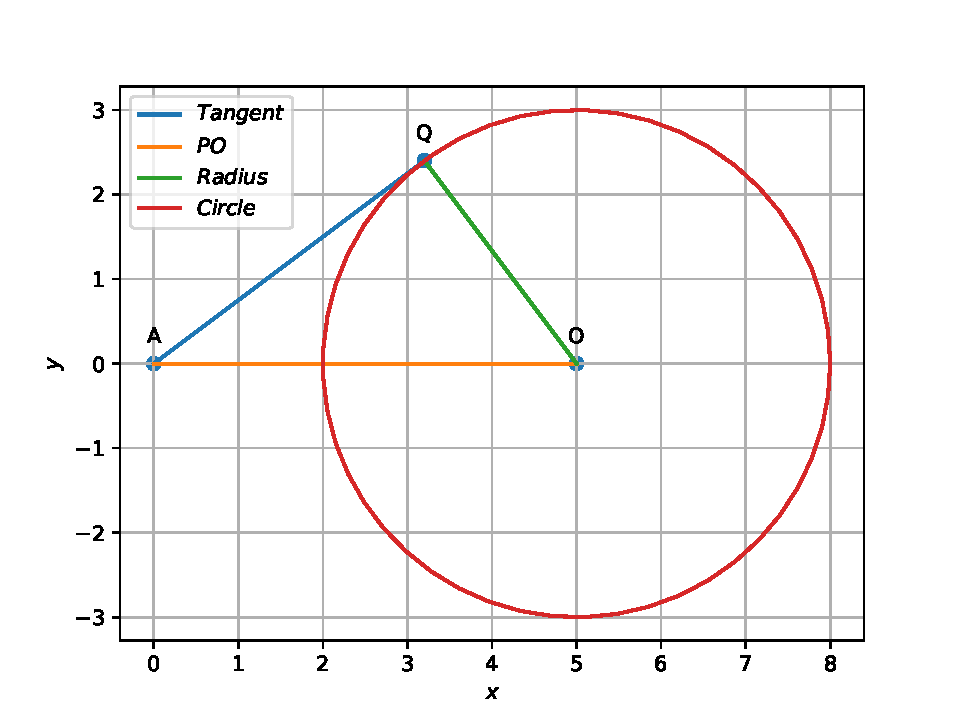
\includegraphics[width=\columnwidth]{chapters/10/10/2/6/figs/circle.pdf}
		\caption{}
		\label{fig:10/10/2/6}
  	\end{figure}
	\\
	\solution
	From the Baudhayana theorem, the radius
\begin{align}
	r =3
\end{align}
%
	Let 
\begin{align}
	\vec{A} = \vec{O} \text{ and } \vec{O} =  \myvec{5\\0} 
\end{align}
The equation of the circle can then be expressed as
\begin{align}
	\norm{\vec{x}}^2+2\vec{u}^{\top}\vec{x} +f = 0
\end{align}
where 
\begin{align}
	\vec{u}  &= - 
	\vec{O} =-  \myvec{5\\0} 
	\\
	f &= \norm{\vec{u}}^2 -r^2 = 16
\end{align}
From 
	  \eqref{eq:h-tangents-sigma},
  \begin{align} 
		\bm{\Sigma} &= 
	   \brak{\vec{A}+\vec{u}}
	  \brak{\vec{A}+\vec{u}}^{\top}
   -
  \brak
  {
  \vec{A}^{\top}\vec{A} + 2\vec{u}^{\top}\vec{A} +f
  }\vec{I}
  \\
	  &=\myvec{9 & 0 \\ 0 & -16}
  \end{align}                    
  Thus,
  from 
  \eqref{eq:quad_form_pair_normvecs-sigma},
  \begin{align} 
	  \vec{P} &= \vec{I}, \lambda_1 = 9, \lambda_2 = -16
	  \\
	  \implies
	  \vec{n}_1 &= \myvec{3 \\[2mm] 4} \quad \text{ and }
  \vec{n}_2 = \myvec{3 \\[2mm] -4}
  \end{align} 
  Substituting  from the above in 
\eqref{eq:conic_tangent_qk-circ},
  \begin{align} 
	\vec{q}_{22} = \frac{1}{5}\myvec{16 \\ 12} = \vec{Q}
\end{align}
in Fig. 
		\ref{fig:10/10/2/6}.
\iffalse
\begin{enumerate}
	\item \textbf{PO = 5cm}
	\item \textbf{PQ = 4cm}
\end{enumerate}
\begin{figure}[h]
\centering
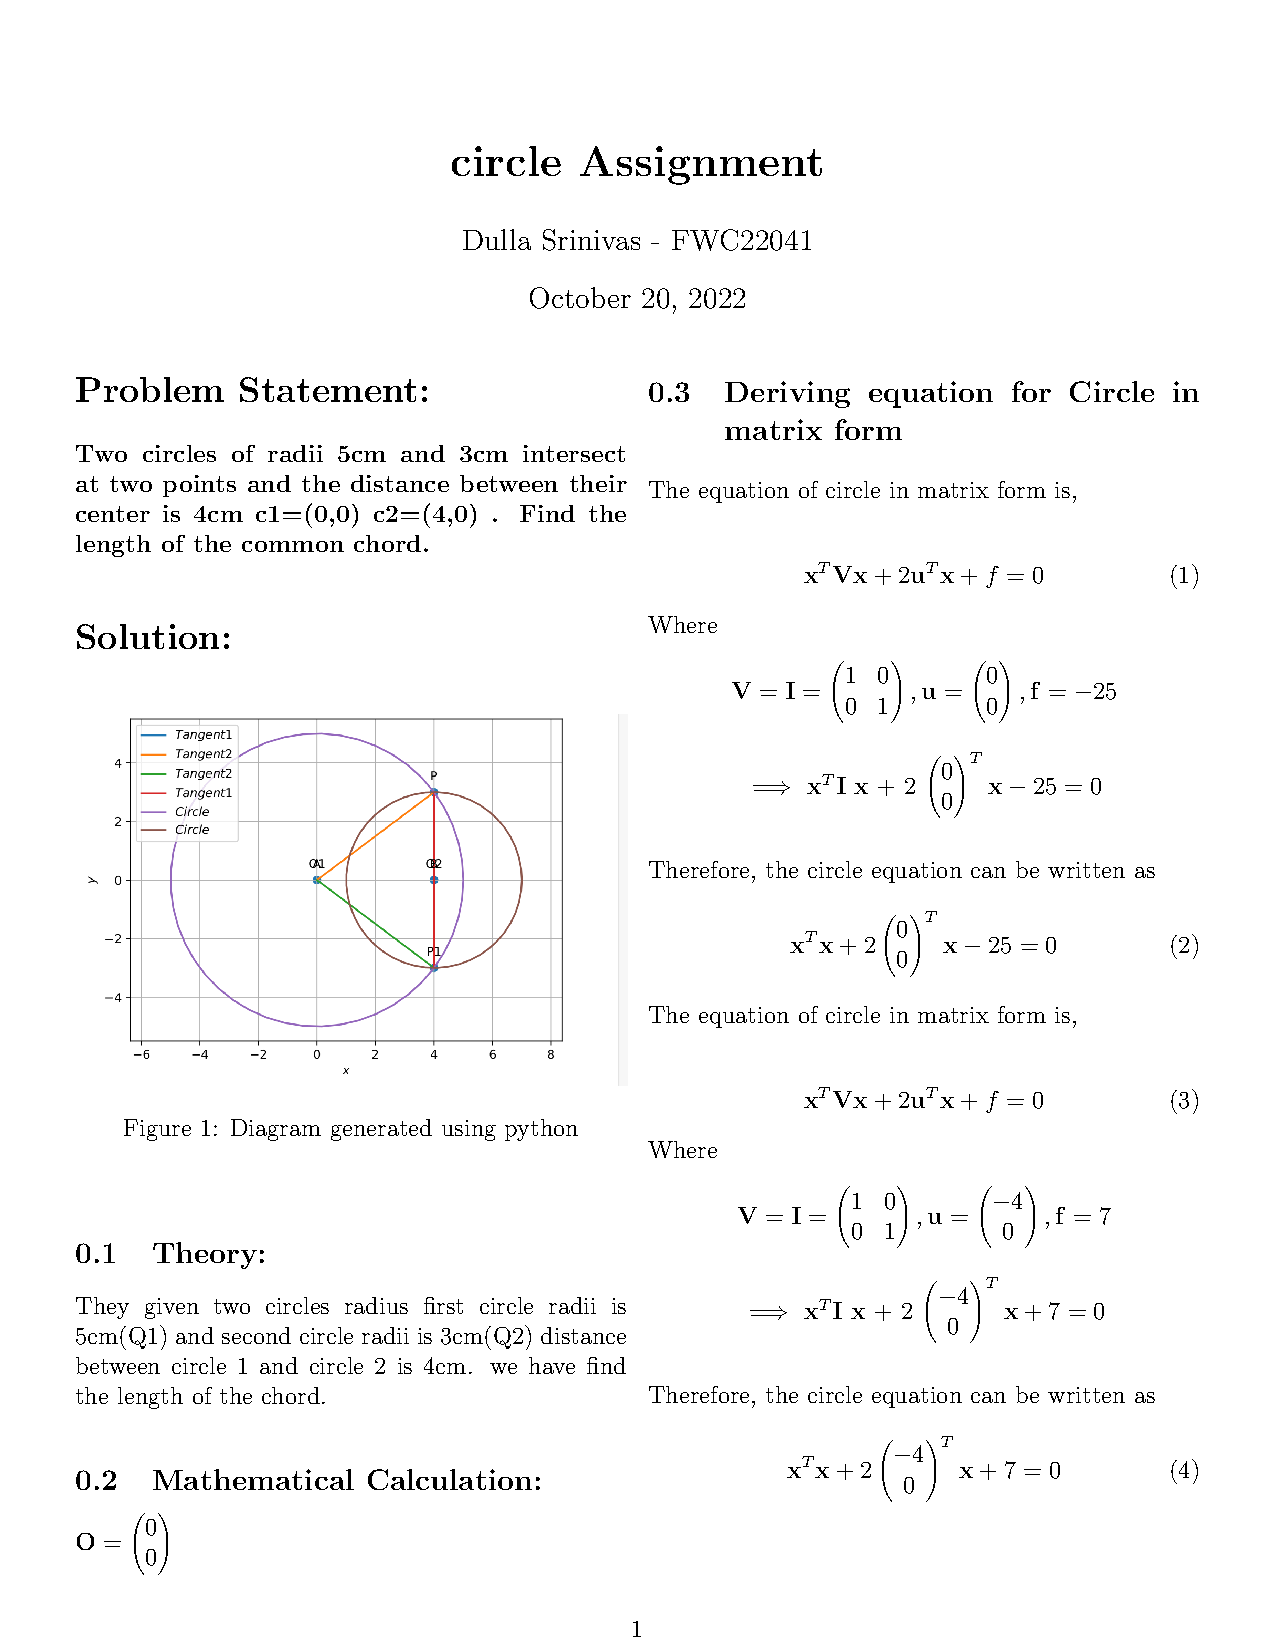
\includegraphics[width=1\columnwidth]{circle.pdf}
\caption{Circle with centre O and a tangent is drawn to circle from point P to Q}
\label{fig:Circle}
\end{figure}

\section*{Solution}
\subsection*{Part 1}
\section*{Construction}
The input parameters are the lengths of AB and AD and angle between AB and ADs \vspace{2mm}\\
{
\setlength\extrarowheight{2pt}
\begin{tabular}{|c|c|c|}
 \hline
 \textbf{Symbol}&\textbf{Value}&\textbf{Description}\\
 \hline
 a&4&PQ\\
 \hline
 d&5&OP\\
 \hline
	$\theta$&$\arccos(4/5)$&$\angle$P\\
 \hline
 0&$d%
 \begin{pmatrix}
  cos(0)\\
  sin(0)\\
 \end{pmatrix}$%
 &centre\\
 \hline
 Q&$a%
 \begin{pmatrix}
  cos\theta\\
  sin\theta\\
 \end{pmatrix}$%
 &point of contact\\
 \hline
\end{tabular}
}
\subsection*{Part 2}
We know that the angle made by tangent and radius of circle at the point of contact is 90 degrees. \\
In order to get the radius of circle consider the triangle $\triangle$PQO \\
\begin{align}
	r = \norm{\vec{O}-\vec{Q}}
\end{align}
\begin{align}
	\norm{\vec{O} - \vec{Q}}= 3
\end{align}
\begin{align}
  r= 3 cm 
\end{align}


Hence the radius of circle is 3cm

\subsection*{Part 3}
Let us proove that the angle made by the tangent and radius at the point of contact is 90  degrees. \\
\begin{enumerate}
	\item OC=OA=3cm
	\item AB = 4cm
\end{enumerate}
\begin{figure}[h]
\centering
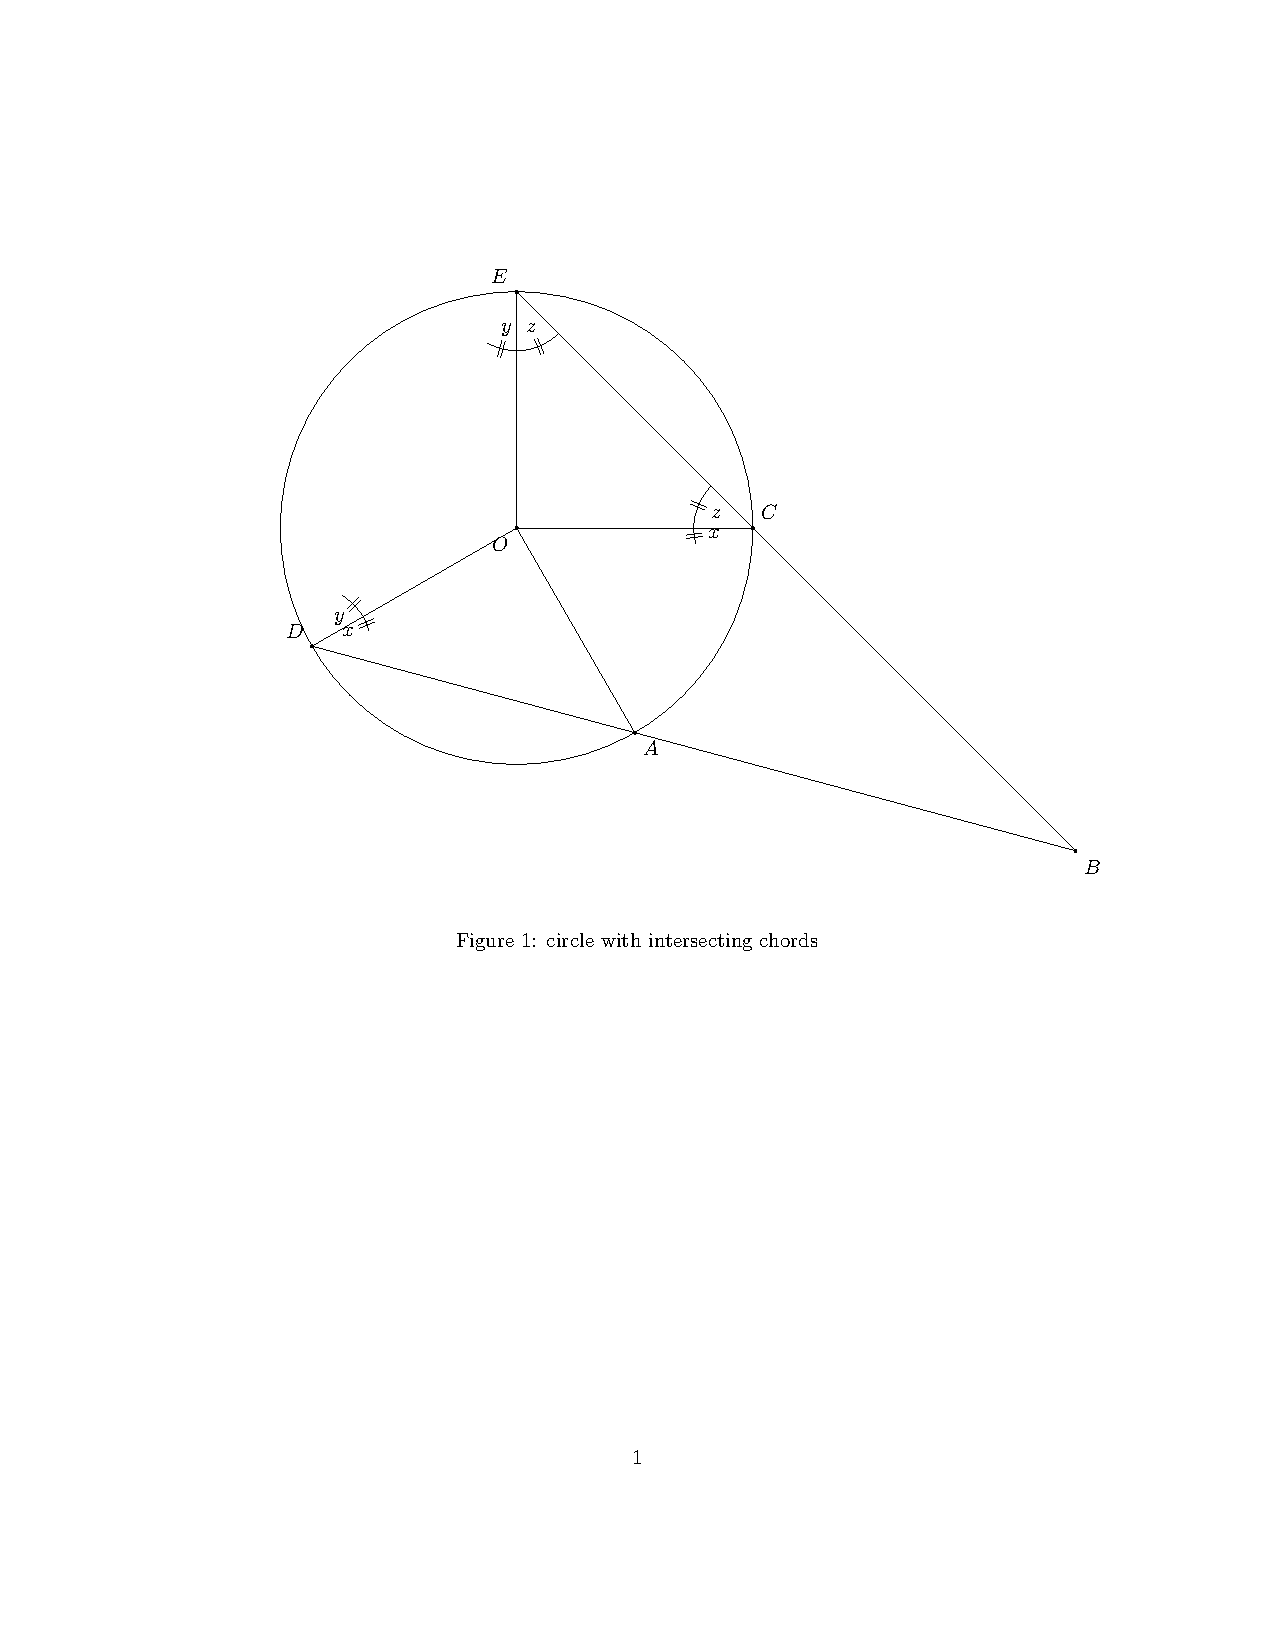
\includegraphics[width=1\columnwidth]{proof.pdf}
\caption{Circle with centre X and a tangent is drawn to circle from point B to A}
\label{fig:Circle}
\end{figure}
From the above figure 
\begin{align}
	\norm{\vec{XB}} = \norm{\vec{XC}} + \norm{\vec{CB}}
\end{align}
\begin{align}
	\norm{\vec{B-X}} = \norm{(\vec{C-X})} + \norm{(\vec{B-C})}
\end{align}
we know that \\
\begin{align}
	\norm{\vec{A-X}} = \norm{\vec{C-X}}
\end{align}
From the above equation we can say that 
\begin{align}
	\norm{\vec{B-X}} > \norm{\vec{A-X}}
\end{align}
From the above result we can conclude that the distance between centre of circle to the any point on the tangent other than point of contact is greater than the distance between the centre to the point of contact. \\
XA is the shortest distance
Hence The distance from centre to the point of contact is shortest distance.\\
Shortest distance of a point from a given line is the perpendicular distance from that line.\\
Hence prooved.
\end{document}
\fi

\item 
\label{chapters/10/10/2/7}
\iffalse
\documentclass[journal,10pt,twocolumn]{article}
\usepackage{graphicx}
\usepackage[margin=0.5in]{geometry}
\usepackage{amsmath}
\usepackage{array}
\usepackage{booktabs}
\usepackage{amssymb}
\title{\textbf{Matrix Assignment}}
\author{lakshmi kamakshi}
\date{September 2022}

\begin{document}

\maketitle
\paragraph{\textit{Problem Statement} -
\fi
Two concentric circles are of radii 5cm and 3cm. Find the length of the chord of the larger circle which touches the smaller circle.
	\begin{figure}[!h]
		\centering
 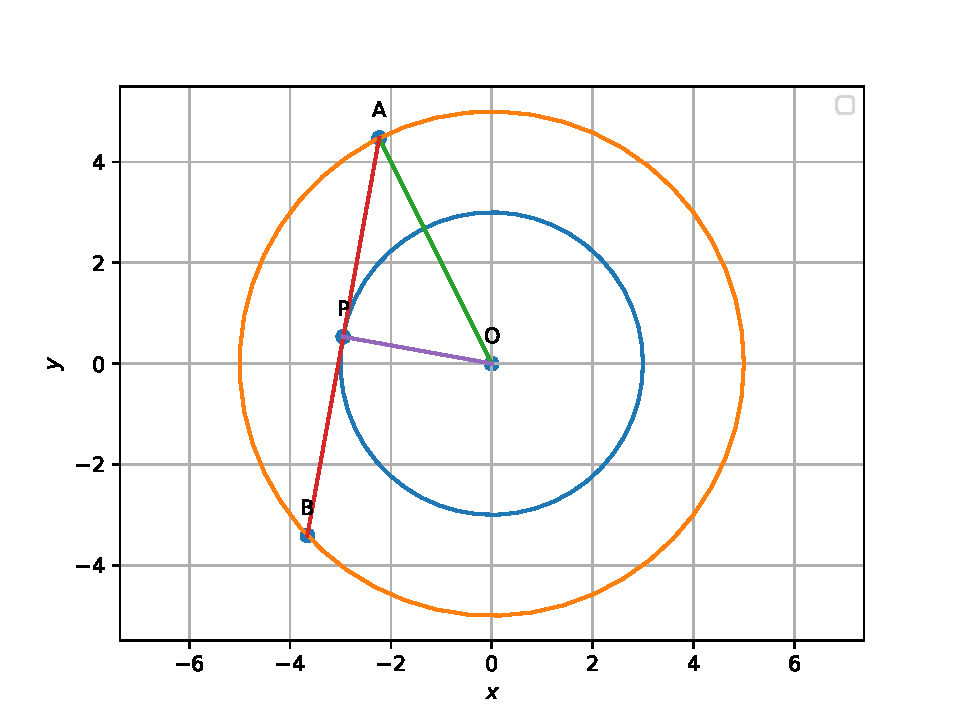
\includegraphics[width=\columnwidth]{chapters/10/10/2/7/figs/fig.pdf}
		\caption{}
		\label{fig:10/10/2/7}
  	\end{figure}
	\\
	\solution  See Fig.
		\ref{fig:10/10/2/7}.  Let 
\begin{align}
	\vec{O} &=
\vec{0}
\\
	r_1 &= 5, r_2 = 3.
\end{align}
Choosing
\begin{align}
	\vec{A} = r_1\myvec{\cos \theta \\ \sin \theta},
\end{align}
$\vec{P}$ can be obtained following the approach in Problem 
\ref{chapters/10/10/2/7}.
From Appendix
	\ref{prop:circ-chord-perp}, $\vec{P}$ is the mid point of $AB$.  This can be used to obtain $\vec{B}$.
\iffalse
\vspace{5mm}

\section*{Solution}

Given the radii of the circles : $3cm$,$5cm$

 r1 = $5cm$ , r2 = $3cm$.
Let,
\begin{eqnarray}
	\boldsymbol{O}-\boldsymbol{A} = \boldsymbol{p}
\\	\boldsymbol{O}-\boldsymbol{P} = \boldsymbol{a}
\\	\boldsymbol{P}-\boldsymbol{A} = \boldsymbol{o}
\end{eqnarray}
\\ From the triangle law of addition of vectors:
\begin{eqnarray}
 \boldsymbol{p} = \boldsymbol{a} + \boldsymbol{o}
\\ \boldsymbol{o} = \boldsymbol{p} - \boldsymbol{a}
\end{eqnarray}
\\ find the magnitude of the vector o 
	\begin{eqnarray}
		||\textbf{o}||^2 = ||\textbf{p-a}||^2
		\\	||\textbf{o}||^2 = |\textbf{p-a}||\textbf{p-a}|^T
		\\||\textbf{o}||^2 = ||\textbf{p}||^2+||\textbf{a}||^2-2\textbf{p.a}^T
		\\ ||\boldsymbol{o}||^2 = \boldsymbol{25 + 9 -2(|\textbf{p}||\textbf{a}|)(cos\theta)}
\end{eqnarray}


\begin{figure}[h]
\includegraphics[width=1\columnwidth]{fig.pdf}
\end{figure}
 From the figure, in $\triangle$ OPA:
\begin{equation}
\boldsymbol{cos\theta} = \boldsymbol{\frac{3}{5}}
\end{equation}
\\ Substitute eqn10 value in eqn9
\begin{eqnarray}
||o||^2 = 34 - 2(3)(5)(\frac{3}{5})
\\ ||o||^2 = 34-18
\\ ||o||^2 = 16
\\ \boldsymbol{||o||} =\boldsymbol{4}
\end{eqnarray}
Similarly, in $\triangle$ OPB,
\begin{eqnarray}
	\boldsymbol{P}-\boldsymbol{B} = \boldsymbol{b}
\\	||\boldsymbol{b}|| = 4
\end{eqnarray}
\begin{eqnarray}
	||\boldsymbol{A-B}|| =|\boldsymbol{o}|+|\boldsymbol{b}|
	\\ \boldsymbol{A-B} = 4+4
	\\ \boldsymbol{A-B} = \boldsymbol{8}
\end{eqnarray}
\\ Therefore, the length of the required chord is $8cm$

\section*{Construction}
The input parameters are the lengths $r_1$ and $r_2$ .\\
\setlength \extrarowheight{2pt}
\centering
	\begin{tabular}{|c|c|c|}
	\hline
	\textbf{symbol}&\textbf{value}&\textbf{description}\\
	\hline
	$r_1$&3&OP\\
	\hline
	$r_2$&5&OA\\
	\hline
		$\theta$&acos($\frac{r_1}{r_2}$)&$\angle$O\\
	\hline
	A&$r_1%
	\begin{pmatrix}
		cos(90 -\theta)\\
		sin(90 -\theta)\\
	\end{pmatrix}$%
	&Point A\\
		\hline
	B&$r_1%
		\begin{pmatrix}
			cos(270+\theta)\\
			-sin(270+\theta)\\
		\end{pmatrix}$%
		&Point B\\
	\hline
\end{tabular}
\end{document}
\fi

\item 
\label{chapters/10/10/2/8}
\iffalse
\documentclass[a4paper,12pt,twocolumn]{article}
\usepackage{graphicx}
\usepackage[margin=0.5in]{geometry}
\usepackage[cmex10]{amsmath}
\usepackage{array}
\usepackage{gensymb}
\usepackage{booktabs}
\title{Circle Assignment}

\author{Ravi Sumanth Muppana- FWC22003}
\date{September 2022}
\providecommand{\norm}[1]{\left\lVert#1\right\rVert}
\providecommand{\abs}[1]{\left\vert#1\right\vert}
\let\vec\mathbf
\newcommand{\myvec}[1]{\ensuremath{\begin{pmatrix}#1\end{pmatrix}}}	
\newcommand{\mydet}[1]{\ensuremath{\begin{vmatrix}#1\end{vmatrix}}}
\providecommand{\brak}[1]{\ensuremath{\left((#1\right)}}
\begin{document}
\maketitle
\section{Problem:}
<<<<<<< HEAD
A quadrilateral $ABCD$ is drawn to circumscribe a circle. Show that $\vec{AB+CD}$ is equal to $\vec{BC+AD}$
=======
\fi
A quadrilateral $ABCD$ is drawn to circumscribe a circle. Show that $AB+CD$ is equal to $BC+AD$
	\begin{figure}[!h]
		\centering
 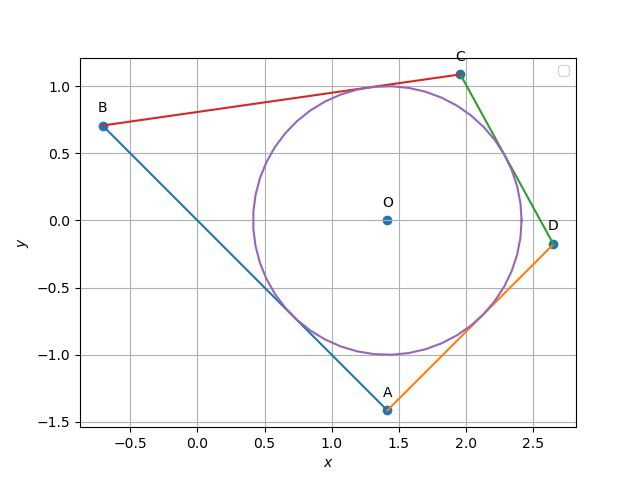
\includegraphics[width=\columnwidth]{chapters/10/10/2/8/figs/circle.png}
		\caption{}
		\label{fig:10/10/2/8}
  	\end{figure}
	\\
	\solution 
	\begin{enumerate}
		\item  Draw the circle.
		\item Choose the point $\vec{A}$.
		\item Draw the tangents from $\vec{A}$ to the circle.
		\item Choose points $\vec{B}, \vec{D}$ on the tangents.
		\item From $\vec{B}, \vec{D}$, draw tangents to the circle intersecting at $\vec{C}$.
	\end{enumerate}
\iffalse
>>>>>>> f531642 (Created codes and figs folder)
\maketitle
\section{Solution:}
\begin{figure}[h]
	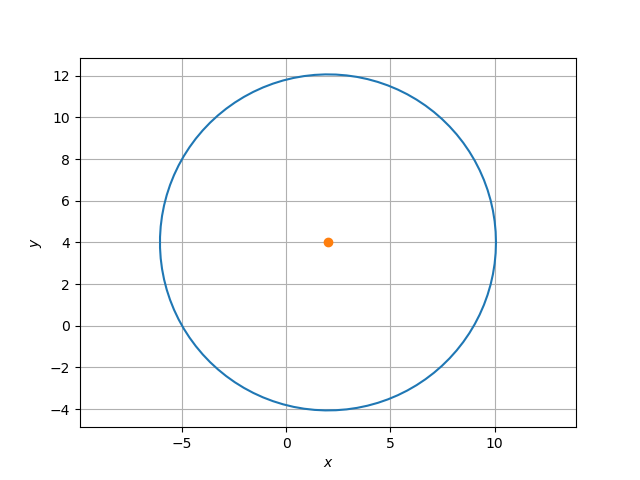
\includegraphics[width=\linewidth]{circle.png}
	\caption{Circle}
\end{figure}
\subsection{Theory:}
The sides of quadrilateral act as tangents to the circle. Also, the tangents at any point is at right angle to the radius of the circle. Let us assume two vectors $\vec{a}$ and $\vec{b}$.
\subsection{Mathematical Calculation:}
The possible tangents to the circle w.r.t vertices are (AP,AQ,BQ,BR,CR,CS,DS,DP). Let us consider the tangents AP,AQ. Their addition vector is $\vec{X}$. The radius of the circle be $\vec{y}$.
\begin{align*}
<<<<<<< HEAD
&\vec{P-A} = \vec{a}\\
&\vec{Q-A} = \vec{b}\\
	&\vec{O-P} = \vec{O-Q} = \vec{y}\\
=======
&\vec{P-A}\\
&\vec{Q-A}\\
	&\vec{O-P} = \vec{O-Q}\\
>>>>>>> f531642 (Created codes and figs folder)
\end{align*}
In triangle APO and AQO,  
\begin{align*}
	&\vec{O-A}= \vec{(O-P)+(P-A)}\\
	&\vec{O-A}= \vec{(O-Q)+(Q-A)}\\
<<<<<<< HEAD
&||\vec{O-A}||^2 = ||\vec{y+a}||^2\\
	&||\vec{O-A}||^2 = ||\vec{y+b}||^2\\
	&||\vec{O-A}||^2 = ||\vec{y}||^2 +2(\vec{y^Ta}) +||\vec{a}||^2\\
&||\vec{O-A}||^2 = ||\vec{y}||^2 +2(\vec{y^Tb}) +||\vec{b}||^2\\
\end{align*}
As $\vec{(y,a)}$ and $\vec{(y,b)}$ are perpendicular to each other, the terms $+2(\vec{y^Ta})$ and $+2(\vec{y^Tb})$ will be equal to zero. 
\begin{align*}
&||\vec{O-A}||^2 = ||\vec{y}||^2 + ||\vec{a}||^2 \\
&||\vec{O-A}||^2 = ||\vec{y}||^2 + ||\vec{b}||^2\\
&||\vec{a}|| = ||\vec{b}||
=======
	&||\vec{O-A}||^2 = ||\vec{(O-P)+(P-A)}||^2\\
	&||\vec{O-A}||^2 = ||\vec{(O-Q)+(Q-A)}||^2\\
	&||\vec{O-A}||^2 = ||\vec{O-P}||^2 +2(\vec{(O-P)^T(P-A)})\\ +||\vec{P-A}||^2\\
	&||\vec{O-A}||^2 = ||\vec{O-Q}||^2 +2(\vec{(O-Q)^T(Q-A)})\\ +||\vec{Q-A}||^2\\
\end{align*}
As $\vec{(O-P),(P-A)}$ and $\vec{(O-Q),(Q-A)}$ are perpendicular to each other, the terms $+2(\vec{(O-P)^T(P-A)})$ and $+2(\vec{(O-Q)^T(Q-A)})$ will be equal to zero. 
\begin{align*}
&||\vec{O-A}||^2 = ||\vec{O-P}||^2 + ||\vec{P-A}||^2 \\
&||\vec{O-A}||^2 = ||\vec{O-Q}||^2 + ||\vec{Q-A}||^2\\
	&||\vec{P-A}|| = ||\vec{Q-A}||
>>>>>>> f531642 (Created codes and figs folder)
\end{align*}
Therefore, the lengths AP is equal to AQ.\\
Similarly, if we take the rest of the tangents as vectors and solve in the same way, we get $BR = BQ$, $CR = CS$, $DP = DS$.
Now, add all the above equations and we get,
\begin{align*}
<<<<<<< HEAD
	&\vec{(AP+BR+CR+DP)} = \vec{(AQ+BQ+CS+DS)}\\
	&\vec{(AD+BC)} = \vec{(AB+CD)}
=======
	&(AP+BR+CR+DP) = (AQ+BQ+CS+DS)\\
	&(AD+BC) = (AB+CD)\\
>>>>>>> f531642 (Created codes and figs folder)
\end{align*}
Hence proved.
\section{Construction:}
The construction of rhombus can be done using only two diagonals, taken as d1 and d2.
\begin{table}
	\centering
\setlength\extrarowheight{2pt}
	\begin{tabular}{|c|c|c|}
		\hline
		\textbf{vertices, variables} & \textbf{formulae} & \textbf{Comments}\\
		\hline
<<<<<<< HEAD
		(a,c,d,r) & (8,3,4,5) & ;sides and radius\\
		\hline
		theta1 & 2*mp.atan(r/d) & angle ADC\\
		\hline
		theta2 & 2*mp.atan(r/a) & angle BAD\\
		\hline                   
		theta3 & 2*mp.atan(r/c) & angle BCD\\
		\hline
		D & (0,0) & vertex D\\
		\hline
		O & (d,r) & centre O\\
		\hline
		C & (c+d)*e1& e1 = (1,0), direction vector\\
		\hline
		A & (a+d)*[(mp.cos(theta1),mp.sin(theta1)] & vertex A\\
		\hline
		m1 & [1, mp.tan(theta1+theta2)] & directional vector\\
		\hline
		B  &  A+lam[0]*m1 & lam = LA.solve(matM,C-A)\\
=======
		O & (1.414,0) & Center\\
		\hline
		r & 1 & radius\\
		\hline
		R & r+d & vertex dist.\\
		\hline
		theta & 270(pi/360) & vertex angle\\
		\hline
		delta1 & 2 & intrsctn dist frm vertex\\
		\hline
		delta2 & 3 & intrsctn dist frm vertex\\
>>>>>>> f531642 (Created codes and figs folder)
		\hline
	\end{tabular}
\end{table}

\end{document}
\fi

\item 
\label{chapters/10/10/2/9}
\iffalse
\documentclass[journal,10pt,twocolumn]{article}
\usepackage{graphicx, float}
\usepackage[margin=0.5in]{geometry}
\usepackage{amsmath, bm}
\usepackage{array}
\usepackage{booktabs}
\providecommand{\norm}[1]{\left\lVert#1\right\rVert}
\let\vec\mathbf
\newcommand{\myvec}[1]{\ensuremath{\begin{pmatrix}#1\end{pmatrix}}}
\newcommand{\mydet}[1]{\ensuremath{\begin{vmatrix}#1\end{vmatrix}}}

\title{\textbf{Circle Assignment}}
\author{Alavala Chinnapa Reddy}
\date{September 2022}

\begin{document}

\maketitle
\paragraph{\textit{Problem Statement} -
\fi
In Fig. 		\ref{fig:10/10/2/9}, $XY$ and $EF$ are two parallel tangents to a circle  with centre $\vec{O}$ and another tangent $AB$ with point of contact $\vec{C}$ intersecting $XY$ at $\vec{A}$ and $EF$ at $\vec{B}$. Prove that $\angle{AOB} = 90\degree$.
	\begin{figure}[!h]
		\centering
 \includegraphics[width=\columnwidth]{chapters/10/10/2/9/figs/c.pdf}
		\caption{}
		\label{fig:10/10/2/9}
  	\end{figure}
	\\
\solution
\iffalse
\section*{\large Solution}

\begin{figure}[H]
\centering
\includegraphics[width=1\columnwidth]{figs/c.pdf}
\caption{Tangents from A to circle through P, C and Tangent from B to circle through Q}
\end{figure}
\section*{Solution}
In order to find the intersection points C and P of tangents from A, the origin is  O. The equation of the circle in the new frame is
\begin{equation}
  \boldsymbol{x}^T\boldsymbol{x} = r^2
\end{equation}

\begin{equation}
	\boldsymbol{x} = \vec{A}+\lambda(\vec{m})
\end{equation}
Sub eq2 in eq1
\begin{equation}
	(\vec{A}+\lambda(\vec{m}))^\top(\vec{A}+\lambda(\vec{m}))=r^2
\end{equation}

Simplify eq3
\begin{equation}
	\lambda^{2}\norm{\boldsymbol{m}}^{2}+2\lambda\vec{A}^\top\vec{m}+\norm{\boldsymbol{A}}^{2}=r^{2}
\end{equation}

Solving eq4
\begin{equation}
	\lambda=\frac{-\vec{A}^\top\vec{m}}{\norm{\boldsymbol{m}}^{2}}  
\end{equation}
\begin{equation}
	(\vec{A}^\top\vec{m})^{2}=(\norm{\boldsymbol{A}}-r^{2})(\norm{\boldsymbol{m}}^{2})
\end{equation}
consider
\begin{equation}
	\vec{m}=\myvec{1\\m}
\end{equation}
From eq6
\begin{eqnarray}
	\vec{A}^\top\vec{m}\vec{m}^\top\vec{A}=\norm{\boldsymbol{m}}^{2}(\norm{\boldsymbol{A}}^{2}-r^{2})\\
	\vec{A}^\top\myvec{1&m\\m&m^{2}}\vec{A}=(1+m^{2})(\norm{\boldsymbol{A}}-r^{2})
\end{eqnarray}
consider
\begin{equation}
	\vec{A}=\myvec{a_1\\a_2}=r_1\myvec{\cos{\theta}\\\sin{\theta}}\\
\end{equation}
sub eq10 in eq9
\begin{eqnarray}
	\myvec{a_1&a_2}\myvec{1&m\\m&m^{2}}\myvec{a_1\\a_2}=(1+m^{2})(\norm{\boldsymbol{A}}^{2}-r^{2})\\
	a_1^{2}+2ma_1a_2+m^{2}a_2^{2}=(1+m^{2})(\norm{\boldsymbol{A}}^{2}-r^{2})\\
	m =  \frac{-a_1a_2\pm\sqrt{r^2\norm{\vec{A}}^2-r^4}}{r^2-a_1^2}
\end{eqnarray}
Solving eq13,we get two values $m_1,m_2$.using $\lambda,m_1,m_2$ find two Points intersecting circle at $\vec{P}$ and $\vec{C}$ from eq2
\begin{eqnarray}
	\vec{m_1}=\myvec{1\\m_1}\\
	\vec{m_2}=\myvec{1\\m_2}\\
	\vec{P}=\vec{A}+\lambda\vec{m_1}\\
	\vec{C}=\vec{A}+\lambda\vec{m_2}
\end{eqnarray}
here $\boldsymbol{O}$ is mid point of $\boldsymbol{P}$ and $\boldsymbol{Q}$
\begin{eqnarray}
	\vec{Q}=2(\vec{O})-\vec{P}
	\end{eqnarray}
	assume 
	\begin{equation}
	\vec{D}=\myvec{0&-1\\1&0}
	\end{equation}
\begin{eqnarray}
	\vec{j} = \vec{D}(\vec{P-A})\\
	\vec{k} =\vec{D}(\vec{A-C})\\
	\vec{C}=\myvec{\vec{j^\top}\\\vec{k^\top}}\myvec{\vec{Q} & \vec{A}}\\
	\vec{B}=\myvec{\vec{j^\top}\\\vec{k^\top}}^{-1}\vec{C}
\end{eqnarray}
Using Parallelogram Law Vector Addition
\begin{equation}
	\vec{A-O}=(\vec{P-O})+(\vec{C-O})    
\end{equation}
\begin{eqnarray}
	\vec{B-O}=(\vec{Q-O})+(\vec{C-O})\\
	\vec{B-O}=-(\vec{O-Q})+(\vec{C-O})
\end{eqnarray}
\begin{equation}
	(\vec{A-O})^\top(\vec{B-O})=((\vec{P-O})+(\vec{C-O}))^\top(-(\vec{O-Q})+(\vec{C-O}))
\end{equation}
We Know
\begin{equation}
    \vec{P-O}=\vec{O-Q}
\end{equation}
From eq27 and eq28
\begin{equation}
	(\vec{O-A})^\top(\vec{O-B})=0
\end{equation}
Finally\\
Dot Product of two  Vectors is Zero\\
then,Angle between those two Vectors is  90$^{\circ}$
\begin{equation}
    \angle{\boldsymbol{AOB}}=\boldsymbol{ 90^{\circ}}
\end{equation}
\section*{\large Construction}
{
\setlength\extrarowheight{5pt}
\begin{tabular}{|c|c|c|}
  \hline
  \textbf{Symbol}&\textbf{Value}&\textbf{Description}\\
  \hline
	$r_1$&4&OA \\
  \hline
	$\theta$&120&\\
  \hline
  r&$3$&Radius\\
  \hline
	$\vec{A}$&$r_1\myvec{cos{\theta}\\sin{\theta}}$&Point A\\[5pt]
	\hline
	$\vec{O}$&$\myvec{0\\0}$&Point O\\[5pt]
	\hline
	$\vec{A_O}$&$\vec{A-O}$&$\vec{A}$ when origin shifted to $\vec{O}$\\[5pt]
  \hline
  $m_1,m_2$&evaluate  eq13 &solution of eq13\\[5pt] 
  \hline
	$\vec{C}$&$\vec{A}+\lambda\vec{m_2}$&Point C\\[5pt]
  \hline
	$\vec{P}$&$\vec{A}+\lambda\vec{m_1}$&Point P\\[5pt]
	\hline
	$\vec{Q}$&2$(\vec{O})-\vec{P}$& Point Q\\
	\hline
	$\vec{B}$&$\myvec{j^\top\\k^\top}\vec{c}$&Point B\\[5pt]
	\hline
\end{tabular}
}
\end{document}
\fi

\item 
\label{chapters/10/10/2/10}
\iffalse
\documentclass[journal,10pt,twocolumn]{article}
\usepackage{graphicx}
\usepackage[margin=0.5in]{geometry}
\usepackage[cmex10]{amsmath}
\usepackage{array}
\usepackage{booktabs}
\title{\textbf{Circle Assignment}}
\author{Bhavani Kanike}
\date{October 2022}

\providecommand{\norm}[1]{\left\lVert#1\right\rVert}
\providecommand{\abs}[1]{\left\vert#1\right\vert}
\let\vec\mathbf
\newcommand{\myvec}[1]{\ensuremath{\begin{pmatrix}#1\end{pmatrix}}}
\newcommand{\mydet}[1]{\ensuremath{\begin{vmatrix}#1\end{vmatrix}}}
\providecommand{\brak}[1]{\ensuremath{\left(#1\right)}}

\begin{document}

\maketitle
\paragraph{\textit{Problem Statement} \\\\-
\fi
Prove that the angle between the two tangents drawn from an external point to a circle is supplementary to the angle subtended by the line-segment joining the points of contact at the centre.
	\begin{figure}[!h]
		\centering
 \includegraphics[width=\columnwidth]{chapters/10/10/2/10/figs/circle1.pdf}
		\caption{}
		\label{fig:10/10/2/10}
  	\end{figure}
	\\
	\solution Follow the approach in Problem 
\ref{chapters/10/10/2/6}
for constructing the tangents to the circle.
\iffalse
}

\section*{\large Solution}

\section*{\large Construction}

\begin{figure}[h]
\centering
\includegraphics[width=1\columnwidth]{circle1.pdf}
\caption{Figure}
\label{fig:triangle}
\end{figure}

The dimensions of the figure is taken as below\\\\
{
\setlength\extrarowheight{2pt}
\centering
	\begin{tabular}{|c|c|}
	\hline
	\textbf{symbol}&\textbf{value}\\
	\hline
	Origin&(0,0)\\
	\hline
	r&4\\
	\hline
	h&(8,6)\\
	\hline
\end{tabular}
}
\\\\\\

TO PROVE :
\begin{equation}
	 \boldsymbol{\angle{AOB} + \angle{AhB} = 180^\circ}
\end{equation}\\
	The equation of a conic with directrix $\vec{n^Tx}$ = c , eccentricity e anf focus $\boldsymbol{f}$ is given by
	
\begin{equation}
	\vec{x}^T\vec{V}\vec{x} + 2\vec{u}^T + f = 0
\end{equation}
	for circle eccentricity e = 0 then,\\
\begin{equation}
	\vec{V} = \vec{I} = \myvec{1&0\\0&1} , \vec{u} = \myvec{0\\0} , f = -r^2
\end{equation}
Point q on conic is given by 
\begin{equation}
	\vec{q} = \vec{V}^{-1}(\vec{n} - \vec{u})
\end{equation}
where, $\vec{n}$ is the normal vectors of the tangents from a point h to the conic are given by 
\begin{equation}
	\vec{n} = \frac{\vec{e_1}}{\vec{e_1^T}h} + \mu_i\vec{Rh}
\end{equation}
\\
where $\mu _i$ 's are given by the following equation
\begin{equation}
	\mu_i = \frac{1}{\vec{m^TVm}}(-\vec{m^T(Vq+u)}	
\end{equation}
	 			$ \pm \sqrt{[\vec{m^T(Vq+u)}]^2 - (\vec{q^TVq + 2u^T }+ f)(\vec{m^TVm)}})$
\\\\
$\mu _i$ 's are obtained by substituting the following in equation 6\\\\
\begin{equation}
	\vec{m = Rh = \myvec{-2\\8}}  ;  \vec{u}  = \myvec{0\\0}  ;  \vec{q} = \frac{\vec{e_1}}{\vec{e_1^T}h}
\end{equation}
 R = $\myvec{-1&1\\1&0}$ 
\\\\
The obtained $\mu_i$'s are substituted in equation 5 and equation 5 is substituted in equation 6 the required points on conic A and B are obtained.\\\\
\section*{Calculation Part}
By Solving equation number 6 using equation number 7 parameters we will get two $\mu_i$ values\\
Therefore ,\\\\
$\mu_i$ =  $\pm 0.488525$\\\\

n1 is obtained by substituting $\mu_i$ = 0.488525\\
n2 is obtained by substituting $\mu_i$ = -0.488525\\

\begin{equation}
	\boldsymbol{n1} = \frac{\myvec{1\\0}}{\myvec{1\\0}^T\myvec{8\\6}} + \mu_1\myvec{0&-1\\1&0}\myvec{8\\6} = \myvec{-0.8\\3.9}
\end{equation}

\begin{equation}
	\boldsymbol{n2} = \frac{\myvec{1\\0}}{\myvec{1\\0}^T\myvec{8\\6}} + \mu_2\myvec{0&-1\\1&0}\myvec{8\\6} = \myvec{3.43\\-2.04}
\end{equation}

\begin{equation}
	\boldsymbol{A} = \myvec{\boldsymbol V}^{-1}\myvec{\boldsymbol{n_1-u}} = \myvec{-0.8\\3.9}
\end{equation}
\begin{equation}
	\boldsymbol{B} = \myvec{\boldsymbol V}^{-1}\myvec{\boldsymbol{n_2-u}} = \myvec{3.43\\-2.04}
\end{equation}
Now the point A and B are formed and tangents are drawn \\\\
To find the angle between AOB and AhB use inner product method \\

\begin{equation}
	\angle AOB = cos^{-1}\frac{(\vec{A}-\vec{O})^T(\vec{B}-\vec{O})}{\norm{(\vec{A}-\vec{O})}\norm{(\vec{B}-\vec{O})}}
\end{equation}\\
\begin{equation}
	\angle AOB = cos^{-1}\frac{\myvec{\myvec{-0.8\\3.9}-\myvec{0\\0}}^T \myvec{\myvec{3.43\\-2.04} - \myvec{0\\0}}}{\norm{\myvec{A-O}} \norm{\myvec{B-O}}}
\end{equation}

\begin{equation}
	\angle AOB = 2.32 radians = 2.32*\frac{180}{\pi} = 133^\circ
\end{equation}
\begin{equation}
	\angle AhB = cos^{-1}\frac{(\vec{h}-\vec{A})^T(\vec{h}-\vec{B})}{\norm{(\vec{h}-\vec{A})}\norm{(\vec{h}-\vec{B})}}
\end{equation}

\begin{equation}
	\angle AhB = cos^{-1}\frac{\myvec{\myvec{8\\6}-\myvec{-0.8\\3.9}}^T \myvec{\myvec{8\\6} - \myvec{3.43\\-2.04}}}{\norm{\myvec{h-A}} \norm{\myvec{h-B}}}
\end{equation}
\begin{equation}
	\angle AhB = 0.82 radians = 0.82*\frac{180}{\pi} = 47^\circ
\end{equation}
If $\angle AOB$ + $\angle AhB$ = 180$^\circ$ then \\
Angle AOB and angle AhB form a supplementary angle.
Therefore,
\begin{equation}
	\boldsymbol{\angle AOB + \angle AhB = 180^\circ}
\end{equation}
\begin{equation}
	\boldsymbol{133^\circ + 47^\circ = 180^\circ}
\end{equation}

\end{document}
\fi

\item 
%\label{chapters/10/10/2/10}
%\iffalse
\documentclass[journal,10pt,twocolumn]{article}
\usepackage{graphicx}
\usepackage[margin=0.5in]{geometry}
\usepackage[cmex10]{amsmath}
\usepackage{array}
\usepackage{booktabs}
\title{\textbf{Circle Assignment}}
\author{Bhavani Kanike}
\date{October 2022}

\providecommand{\norm}[1]{\left\lVert#1\right\rVert}
\providecommand{\abs}[1]{\left\vert#1\right\vert}
\let\vec\mathbf
\newcommand{\myvec}[1]{\ensuremath{\begin{pmatrix}#1\end{pmatrix}}}
\newcommand{\mydet}[1]{\ensuremath{\begin{vmatrix}#1\end{vmatrix}}}
\providecommand{\brak}[1]{\ensuremath{\left(#1\right)}}

\begin{document}

\maketitle
\paragraph{\textit{Problem Statement} \\\\-
\fi
Prove that the angle between the two tangents drawn from an external point to a circle is supplementary to the angle subtended by the line-segment joining the points of contact at the centre.
	\begin{figure}[!h]
		\centering
 \includegraphics[width=\columnwidth]{chapters/10/10/2/10/figs/circle1.pdf}
		\caption{}
		\label{fig:10/10/2/10}
  	\end{figure}
	\\
	\solution Follow the approach in Problem 
\ref{chapters/10/10/2/6}
for constructing the tangents to the circle.
\iffalse
}

\section*{\large Solution}

\section*{\large Construction}

\begin{figure}[h]
\centering
\includegraphics[width=1\columnwidth]{circle1.pdf}
\caption{Figure}
\label{fig:triangle}
\end{figure}

The dimensions of the figure is taken as below\\\\
{
\setlength\extrarowheight{2pt}
\centering
	\begin{tabular}{|c|c|}
	\hline
	\textbf{symbol}&\textbf{value}\\
	\hline
	Origin&(0,0)\\
	\hline
	r&4\\
	\hline
	h&(8,6)\\
	\hline
\end{tabular}
}
\\\\\\

TO PROVE :
\begin{equation}
	 \boldsymbol{\angle{AOB} + \angle{AhB} = 180^\circ}
\end{equation}\\
	The equation of a conic with directrix $\vec{n^Tx}$ = c , eccentricity e anf focus $\boldsymbol{f}$ is given by
	
\begin{equation}
	\vec{x}^T\vec{V}\vec{x} + 2\vec{u}^T + f = 0
\end{equation}
	for circle eccentricity e = 0 then,\\
\begin{equation}
	\vec{V} = \vec{I} = \myvec{1&0\\0&1} , \vec{u} = \myvec{0\\0} , f = -r^2
\end{equation}
Point q on conic is given by 
\begin{equation}
	\vec{q} = \vec{V}^{-1}(\vec{n} - \vec{u})
\end{equation}
where, $\vec{n}$ is the normal vectors of the tangents from a point h to the conic are given by 
\begin{equation}
	\vec{n} = \frac{\vec{e_1}}{\vec{e_1^T}h} + \mu_i\vec{Rh}
\end{equation}
\\
where $\mu _i$ 's are given by the following equation
\begin{equation}
	\mu_i = \frac{1}{\vec{m^TVm}}(-\vec{m^T(Vq+u)}	
\end{equation}
	 			$ \pm \sqrt{[\vec{m^T(Vq+u)}]^2 - (\vec{q^TVq + 2u^T }+ f)(\vec{m^TVm)}})$
\\\\
$\mu _i$ 's are obtained by substituting the following in equation 6\\\\
\begin{equation}
	\vec{m = Rh = \myvec{-2\\8}}  ;  \vec{u}  = \myvec{0\\0}  ;  \vec{q} = \frac{\vec{e_1}}{\vec{e_1^T}h}
\end{equation}
 R = $\myvec{-1&1\\1&0}$ 
\\\\
The obtained $\mu_i$'s are substituted in equation 5 and equation 5 is substituted in equation 6 the required points on conic A and B are obtained.\\\\
\section*{Calculation Part}
By Solving equation number 6 using equation number 7 parameters we will get two $\mu_i$ values\\
Therefore ,\\\\
$\mu_i$ =  $\pm 0.488525$\\\\

n1 is obtained by substituting $\mu_i$ = 0.488525\\
n2 is obtained by substituting $\mu_i$ = -0.488525\\

\begin{equation}
	\boldsymbol{n1} = \frac{\myvec{1\\0}}{\myvec{1\\0}^T\myvec{8\\6}} + \mu_1\myvec{0&-1\\1&0}\myvec{8\\6} = \myvec{-0.8\\3.9}
\end{equation}

\begin{equation}
	\boldsymbol{n2} = \frac{\myvec{1\\0}}{\myvec{1\\0}^T\myvec{8\\6}} + \mu_2\myvec{0&-1\\1&0}\myvec{8\\6} = \myvec{3.43\\-2.04}
\end{equation}

\begin{equation}
	\boldsymbol{A} = \myvec{\boldsymbol V}^{-1}\myvec{\boldsymbol{n_1-u}} = \myvec{-0.8\\3.9}
\end{equation}
\begin{equation}
	\boldsymbol{B} = \myvec{\boldsymbol V}^{-1}\myvec{\boldsymbol{n_2-u}} = \myvec{3.43\\-2.04}
\end{equation}
Now the point A and B are formed and tangents are drawn \\\\
To find the angle between AOB and AhB use inner product method \\

\begin{equation}
	\angle AOB = cos^{-1}\frac{(\vec{A}-\vec{O})^T(\vec{B}-\vec{O})}{\norm{(\vec{A}-\vec{O})}\norm{(\vec{B}-\vec{O})}}
\end{equation}\\
\begin{equation}
	\angle AOB = cos^{-1}\frac{\myvec{\myvec{-0.8\\3.9}-\myvec{0\\0}}^T \myvec{\myvec{3.43\\-2.04} - \myvec{0\\0}}}{\norm{\myvec{A-O}} \norm{\myvec{B-O}}}
\end{equation}

\begin{equation}
	\angle AOB = 2.32 radians = 2.32*\frac{180}{\pi} = 133^\circ
\end{equation}
\begin{equation}
	\angle AhB = cos^{-1}\frac{(\vec{h}-\vec{A})^T(\vec{h}-\vec{B})}{\norm{(\vec{h}-\vec{A})}\norm{(\vec{h}-\vec{B})}}
\end{equation}

\begin{equation}
	\angle AhB = cos^{-1}\frac{\myvec{\myvec{8\\6}-\myvec{-0.8\\3.9}}^T \myvec{\myvec{8\\6} - \myvec{3.43\\-2.04}}}{\norm{\myvec{h-A}} \norm{\myvec{h-B}}}
\end{equation}
\begin{equation}
	\angle AhB = 0.82 radians = 0.82*\frac{180}{\pi} = 47^\circ
\end{equation}
If $\angle AOB$ + $\angle AhB$ = 180$^\circ$ then \\
Angle AOB and angle AhB form a supplementary angle.
Therefore,
\begin{equation}
	\boldsymbol{\angle AOB + \angle AhB = 180^\circ}
\end{equation}
\begin{equation}
	\boldsymbol{133^\circ + 47^\circ = 180^\circ}
\end{equation}

\end{document}
\fi

\item 
\label{chapters/10/10/2/12}
\iffalse
\documentclass[a4paper,12pt,twocolumn]{article}
\usepackage{graphicx}
\usepackage[margin=0.5in]{geometry}
\usepackage[cmex10]{amsmath}
\usepackage{array}
\usepackage{gensymb}
\usepackage{booktabs}
\usepackage{tabularx}
\title{Circle Assignment}

\author{Ginna Shreyani- FWC22006}
\date{September 2022}
\providecommand{\norm}[1]{\left\lVert#1\right\rVert}
\providecommand{\abs}[1]{\left\vert#1\right\vert}
\let\vec\mathbf
\newcommand{\myvec}[1]{\ensuremath{\begin{pmatrix}#1\end{pmatrix}}}	
\newcommand{\mydet}[1]{\ensuremath{\begin{vmatrix}#1\end{vmatrix}}}
\providecommand{\brak}[1]{\ensuremath{\left((#1\right)}}
\begin{document}
\maketitle
\section{Problem:}
\fi
A triangle $ABC$ is drawn to circumscribe a circle of radius 4cm such that the segments $BD$ and $DC$ into which $BC$ is divided by the point of contact $D$ are of lengths 8cm and 6cm respectively. Find the sides $AB$ and $AC$.
	\begin{figure}[!h]
		\centering
 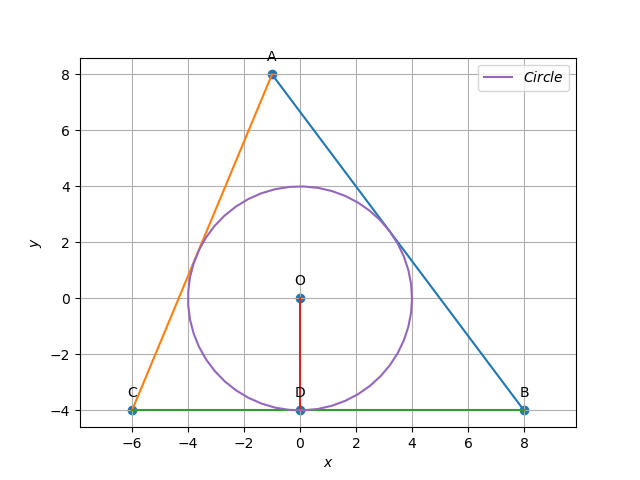
\includegraphics[width=\columnwidth]{chapters/10/10/2/12/figs/circle.png}
		\caption{}
		\label{fig:10/10/2/12}
  	\end{figure}
\iffalse
\begin{figure}[h]
       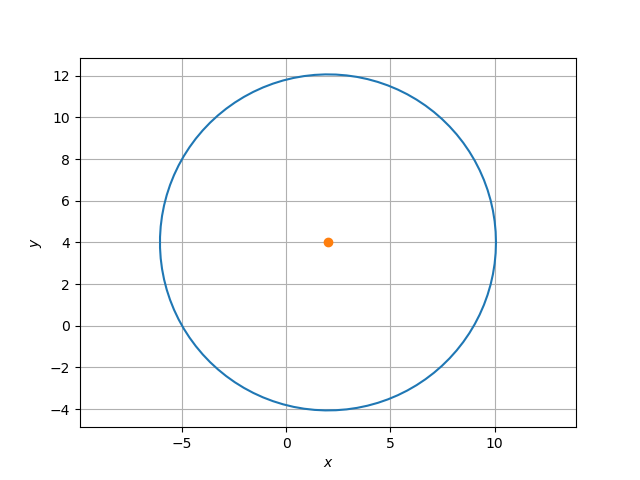
\includegraphics[width=\linewidth]{circle.png}
\end{figure}
\section{Construction:}
\begin{tabularx}
{0.45\textwidth}{
|>
{\raggedright\arraybackslash}X
|>
{\centering\arraybackslash}X
|>
{\raggedleft\arraybackslash}X
|}
\hline
 Variable & Point/Length & Description\\
\hline
  r & 4cm &Radius of the given circle\\
 \hline
  C & $\myvec{0\\0}$ & Origin\\
 \hline
 c & 6cm &Distance from Vertex C to point D\\
 \hline
  D &$\myvec{c\\0}$&Point on side BC\\
 \hline
 O &$\myvec{c\\r}$&Center of the circle\\
 \hline
  CB & $\myvec{c+b\\0}$ & Vertex B\\
 \hline
\end{tabularx}
\section{Solution:}
\subsection{Theory:}
\subsection{Mathematical Calculation:}
\begin{figure}[h]
    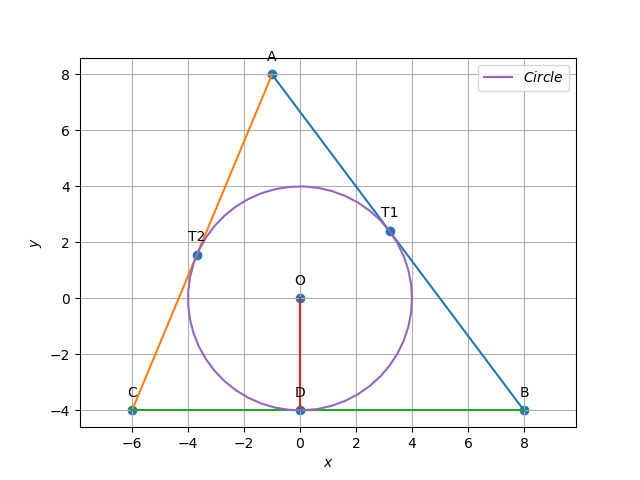
\includegraphics[width=\linewidth]{circle1.png}
\end{figure}
\\
\solution
Let us assume that the center of the circle is origin and point D lies on Y-axis.\\
Therefore, we can get the points B and C.\\
\begin{align*}
	&D = \myvec{0\\-4}\\
	&B = \myvec{8\\-4}\\
	&C = \myvec{-6\\-4}
\end{align*}
Here point C acts as external point from which tangents can be drawn to the circle.The direction vector $\vec{m}$ satisy the equation\\
\begin{align*}
	&\vec{m^T}\vec{\Sigma}\vec{m} = 0
\end{align*}
Assuming the external point as h,$\vec{\Sigma}$ is given as\\
\begin{align*}
	&\vec{\Sigma} = \brak{\vec{Vh}+\vec{u}}\brak{\vec{Vh}+\vec{u}}^T - \brak{\vec{h}^T\vec{V}\vec{h} + 2\vec{u}^T\vec{h} + f}\vec{V}
\end{align*}
$\vec{\Sigma}$ can be orthogonally  diagonalized as\\
\begin{align}
	&\vec{\Sigma} = \vec{\Gamma}^T\vec{D}\vec{\Gamma}\\
	\label{eq:eigenvalV}
	&\vec{D} = \myvec{\lambda_1 & 0\\0 & \lambda_2}\\
	\label{eq:eigenvecP}
	&\vec{\Gamma} = \myvec{\vec{y}_1 & \vec{y}_2}, \quad \vec{\Gamma}^T=\vec{\Gamma}^{-1}
\end{align}
Using \eqref{eq:eigenvalV} and \eqref{eq:eigenvecP} and substituting $\vec{h}$ as $\vec{C}$, the normal vector $\vec{n}$ of the tangent drawn from $\vec{C}$ can be written as\\
\begin{align}
	\label{eq:tangent_normal}
	&\vec{n} = \vec{\Gamma}\myvec{\sqrt{\abs{\lambda_1}} \\\\ \pm\sqrt{\abs{\lambda_2}}}
\end{align}
Using the vectors $\vec{n}$ in \eqref{eq:tangent_normal}, the direction vectors $\vec{m}$ can be found in 2-dimensional space since they are orthogonal. The points of contact of the tangents are given by
\begin{align*}
	&\vec{T}_i = \vec{C} - \frac{\vec{m}^T\brak{\vec{VC}+\vec{u}}}{\vec{m}^T\vec{V}\vec{m}}
\end{align*}
Similarly we can find the contact point from vertex B.\\
Since, we have all the contact points we can get the line equations of $\vec{A-C}$ and $\vec{A-B}$
\begin{align*}
	&\vec{n}^T\vec{X-T_i}= 0
\end{align*}
The intersection of these two lines is vertex A. Since, we know all the vertices of the given triangle the length of AB and AC can be calculated.\\
Therefore, length of AB is $\vec{||A-B||}$\\
and length of AC is $\vec{||A-C||}$
\end{document}
\fi

 \item Prove that opposite sides of a quadrilateral circumscribing a circle 
    subtend supplementary angles at the centre of the circle.
\label{chapters/10/10/2/13}
\\
       \solution 
\iffalse
\documentclass[journal,12pt,twocolumn]{IEEEtran}
\usepackage{setspace}
\usepackage{gensymb}
\usepackage{xcolor}
\usepackage{caption}
\singlespacing
\usepackage{siunitx}
\usepackage[cmex10]{amsmath}
\usepackage{mathtools}
\usepackage{hyperref}
\usepackage{amsthm}
\usepackage{mathrsfs}
\usepackage{txfonts}
\usepackage{stfloats}
\usepackage{cite}
\usepackage{cases}
\usepackage{subfig}
\usepackage{longtable}
\usepackage{multirow}
\usepackage{enumitem}
\usepackage{bm}
\usepackage{mathtools}
\usepackage{listings}
\usepackage{tikz}
\usetikzlibrary{shapes,arrows,positioning}
\usepackage{circuitikz}
\renewcommand{\vec}[1]{\boldsymbol{\mathbf{#1}}}
\DeclareMathOperator*{\Res}{Res}
\renewcommand\thesection{\arabic{section}}
\renewcommand\thesubsection{\thesection.\arabic{subsection}}
\renewcommand\thesubsubsection{\thesubsection.\arabic{subsubsection}}

\renewcommand\thesectiondis{\arabic{section}}
\renewcommand\thesubsectiondis{\thesectiondis.\arabic{subsection}}
\renewcommand\thesubsubsectiondis{\thesubsectiondis.\arabic{subsubsection}}
\hyphenation{op-tical net-works semi-conduc-tor}

\lstset{
language=Python,
frame=single, 
breaklines=true,
columns=fullflexible
}
\begin{document}
\theoremstyle{definition}
\newtheorem{theorem}{Theorem}[section]
\newtheorem{problem}{Problem}
\newtheorem{proposition}{Proposition}[section]
\newtheorem{lemma}{Lemma}
\newtheorem{corollary}[theorem]{Corollary}
\newtheorem{example}{Example}[section]
\newtheorem{definition}{Definition}[section]
\newcommand{\BEQA}{\begin{eqnarray}}
\newcommand{\EEQA}{\end{eqnarray}}
\newcommand{\define}{\stackrel{\triangle}{=}}
\newcommand{\myvec}[1]{\ensuremath{\begin{pmatrix}#1\end{pmatrix}}}
\newcommand{\mydet}[1]{\ensuremath{\begin{vmatrix}#1\end{vmatrix}}}
\bibliographystyle{IEEEtran}
\providecommand{\nCr}[2]{\,^{#1}C_{#2}} % nCr
\providecommand{\nPr}[2]{\,^{#1}P_{#2}} % nPr
\providecommand{\mbf}{\mathbf}
\providecommand{\pr}[1]{\ensuremath{\Pr\left(#1\right)}}
\providecommand{\qfunc}[1]{\ensuremath{Q\left(#1\right)}}
\providecommand{\sbrak}[1]{\ensuremath{{}\left[#1\right]}}
\providecommand{\lsbrak}[1]{\ensuremath{{}\left[#1\right.}}
\providecommand{\rsbrak}[1]{\ensuremath{{}\left.#1\right]}}
\providecommand{\brak}[1]{\ensuremath{\left(#1\right)}}
\providecommand{\lbrak}[1]{\ensuremath{\left(#1\right.}}
\providecommand{\rbrak}[1]{\ensuremath{\left.#1\right)}}
\providecommand{\cbrak}[1]{\ensuremath{\left\{#1\right\}}}
\providecommand{\lcbrak}[1]{\ensuremath{\left\{#1\right.}}
\providecommand{\rcbrak}[1]{\ensuremath{\left.#1\right\}}}
\theoremstyle{remark}
\newtheorem{rem}{Remark}
\newcommand{\sgn}{\mathop{\mathrm{sgn}}}
\newcommand{\rect}{\mathop{\mathrm{rect}}}
\newcommand{\sinc}{\mathop{\mathrm{sinc}}}
\providecommand{\abs}[1]{\left\vert#1\right\vert}
\providecommand{\res}[1]{\Res\displaylimits_{#1}} 
\providecommand{\norm}[1]{\left\Vert#1\right\Vert}
\providecommand{\mtx}[1]{\mathbf{#1}}
\providecommand{\mean}[1]{E\left[ #1 \right]}
\providecommand{\fourier}{\overset{\mathcal{F}}{ \rightleftharpoons}}
\providecommand{\ztrans}{\overset{\mathcal{Z}}{ \rightleftharpoons}}
\providecommand{\system}[1]{\overset{\mathcal{#1}}{ \longleftrightarrow}}
\newcommand{\solution}{\noindent \textbf{Solution: }}
\providecommand{\dec}[2]{\ensuremath{\overset{#1}{\underset{#2}{\gtrless}}}}
\let\StandardTheFigure\thefigure
\def\putbox#1#2#3{\makebox[0in][l]{\makebox[#1][l]{}\raisebox{\baselineskip}[0in][0in]{\raisebox{#2}[0in][0in]{#3}}}}
     \def\rightbox#1{\makebox[0in][r]{#1}}
     \def\centbox#1{\makebox[0in]{#1}}
     \def\topbox#1{\raisebox{-\baselineskip}[0in][0in]{#1}}
     \def\midbox#1{\raisebox{-0.5\baselineskip}[0in][0in]{#1}}

\vspace{3cm}
\title{Circle Assignment}
\author{Gautam Singh}
\maketitle
\bigskip

\begin{abstract}
    This document contains the solution to Question 13 of 
    Exercise 2 in Chapter 10 of the class 10 NCERT textbook.
\end{abstract}

\begin{enumerate}
       \solution 
\fi
		We begin by proving a useful lemma.
    \begin{lemma}
        The line joining the centre of the circle to an external point bisects
        the angle subtended by the tangent chord at the centre.
    \end{lemma}
    \begin{proof}
        Refer to Fig. \ref{fig:chapters/10/10/2/13/tangent}.
 Set $\vec{O}$ to be the origin. Since 
        $OA \perp AP$,
        \begin{align}
            \vec{A}^\top\brak{\vec{A}-\vec{P}} &= 0 \\
            \implies \vec{A}^\top\vec{P} &= \norm{\vec{A}}^2
            \label{eq:chapters/10/10/2/13/a-p}
        \end{align}
        Similarly,
        \begin{align}
            \vec{B}^\top\vec{P} = \norm{\vec{B}}^2
            \label{eq:chapters/10/10/2/13/b-p}
        \end{align}
        Since $\vec{A}$ and $\vec{B}$ lie on the circle, their norms are equal.
        Thus, from \eqref{eq:chapters/10/10/2/13/a-p} and \eqref{eq:chapters/10/10/2/13/b-p},
        \begin{align}
            \vec{A}^\top\vec{P} = \vec{B}^\top\vec{P}
        \end{align}
        and the lemma follows.
        \begin{figure}[!ht]
            \centering
            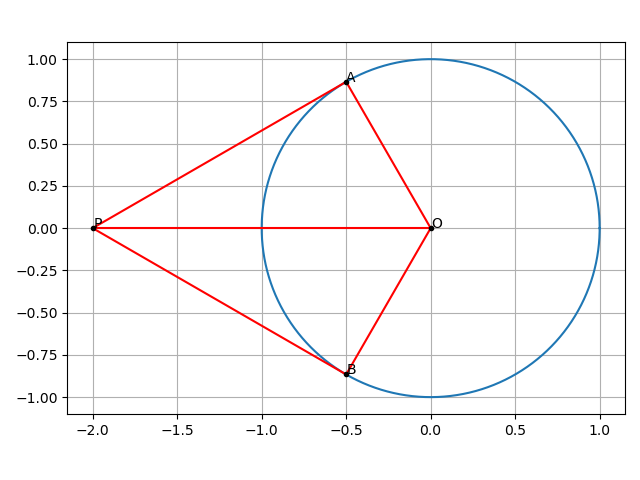
\includegraphics[width=\columnwidth]{chapters/10/10/2/13/figs/tangent.png}
            \caption{$OP$ bisects $\angle AOB$.}
            \label{fig:chapters/10/10/2/13/tangent}
        \end{figure}
    \end{proof}
    Call the quadrilateral $ABCD$, where
    \begin{align}
        \vec{A} = \myvec{-2\\0},\ \vec{C} = \myvec{1\\1}
        \label{eq:chapters/10/10/2/13/a-c-def}
    \end{align}
    Suppose that $ABCD$ circumscribes the unit circle, given by
    \begin{align}
        \vec{x}^\top\vec{x} - 1 = 0
        \label{eq:chapters/10/10/2/13/unit-circ}
    \end{align}
    Comparing \eqref{eq:chapters/10/10/2/13/unit-circ} with the general equation of the circle,
    \begin{align}
        \vec{u} = \vec{0},\ f = -1
        \label{eq:chapters/10/10/2/13/u-f-val}
    \end{align}
    To find the points of contact from $\vec{A}$, we have
    \begin{align}
        \vec{\Sigma_A} &= \brak{\vec{A}+\vec{u}}\brak{\vec{A}+\vec{u}}^\top - \brak{\vec{A}^\top\vec{A}+2\vec{u}^\top\vec{A} + f}\vec{I} \\
                     &= \myvec{1&0\\0&-3}
                     \label{eq:chapters/10/10/2/13/sigma}
    \end{align}
    The eigenvalues of $\vec{\Sigma_A}$ are
    \begin{align}
        \lambda_1 = 1,\ \lambda_2 = -3
        \label{eq:chapters/10/10/2/13/lambda}
    \end{align}
    and since the eigenvector matrix $\vec{P_A} = \vec{I}$,
    \begin{align}
        \vec{n_1} = \myvec{1\\\sqrt{3}},\ \vec{n_2} = \myvec{1\\-\sqrt{3}}
        \label{eq:chapters/10/10/2/13/n-sigma}
    \end{align}
    Thus, the points of contact are given by
    \begin{align}
        \vec{E} = \frac{1}{2}\myvec{-1\\\sqrt{3}},\ \vec{H} = \frac{1}{2}\myvec{-1\\-\sqrt{3}}
        \label{eq:chapters/10/10/2/13/poc-eh}
    \end{align}
    Similarly for $\vec{C}$,
    \begin{align}
        \vec{\Sigma_C} = \myvec{1&1\\1&1} - \vec{I} = \myvec{0&1\\1&0}
    \end{align}
    Notice that
    \begin{align}
        \vec{\Sigma_C}\myvec{1\\1} &= \myvec{1\\1} \\
        \vec{\Sigma_C}\myvec{1\\-1} &= -\myvec{1\\-1} \\
    \end{align}
    Thus, the eigenvalues and the corresponding eigenvector
    matrix is
    \begin{align}
        \mu_1 = 1,\ \mu_2 = -1,\ \vec{P_C} = \myvec{1&1\\1&-1}
    \end{align}
    and thus
    \begin{align}
        \vec{m_1} &= \vec{P_C}\myvec{1\\1} = \myvec{2\\0} \\ 
        \vec{m_2} &= \vec{P_C}\myvec{1\\-1} = \myvec{0\\2}
    \end{align}
    Therefore, the points of contact of $\vec{C}$ are
    \begin{align}
        \vec{F} = \myvec{1\\0},\ \vec{G} = \myvec{0\\1}
        \label{eq:chapters/10/10/2/13/poc-fg}
    \end{align}
    Using the lemma we proved above, the direction vectors of $\vec{B}$ and 
    $\vec{D}$ are
    \begin{align}
        \vec{d_B} &= \vec{E} + \vec{F} = \frac{\sqrt{3}}{2}\myvec{\sqrt{3}\\1} \label{eq:chapters/10/10/2/13/d-B} \\
        \vec{d_D} &= \vec{G} + \vec{H} = \frac{1}{2}\myvec{-1\\2-\sqrt{3}} \label{eq:chapters/10/10/2/13/d-D}
    \end{align}
    Clearly,
    \begin{align}
        \norm{\vec{d_B}} &= \sqrt{3} \\
        \norm{\vec{d_D}} &= \sqrt{2-\sqrt{3}}
        \label{eq:chapters/10/10/2/13/norm-d}
    \end{align}
    and from \eqref{eq:chapters/10/10/2/13/a-c-def}, \eqref{eq:chapters/10/10/2/13/d-B} and \eqref{eq:chapters/10/10/2/13/d-D},
    \begin{align}
        \cos\angle AOD &= \frac{\vec{A}^\top\vec{d_D}}{\norm{A}\norm{\vec{d_D}}} \\
                       &= \frac{-1}{2\sqrt{2\sqrt{3}}} \\
                       &= -\frac{\sqrt{2+\sqrt{3}}}{2} \\
                       &= -\frac{\sqrt{3}+1}{2\sqrt{2}} \label{eq:chapters/10/10/2/13/cos-aod} \\
        \cos\angle BOC &= \frac{\vec{C}^\top\vec{d_B}}{\norm{C}\norm{\vec{d_B}}} \\
                       &= \frac{\sqrt{3}+1}{2\sqrt{2}} \label{eq:chapters/10/10/2/13/cos-boc}
    \end{align}
    Hence, from \eqref{eq:chapters/10/10/2/13/norm-d}, \eqref{eq:chapters/10/10/2/13/cos-aod} and \eqref{eq:chapters/10/10/2/13/cos-boc},
    \begin{align}
        \cos\angle AOD + \cos\angle BOC = 0
    \end{align}
    and hence, $\angle AOD + \angle BOC = \pi$, as required.

    The situation is illustrated in Fig. \ref{fig:chapters/10/10/2/13/quad-circ}. The numerical parameters used 
    in the construction are shown in Table \ref{tab:chapters/10/10/2/13/param}.
    \begin{table}[!ht]
        \centering
        \begin{tabular}{|c|c|}
            \hline
            \textbf{Parameter} & \textbf{Value} \\
            \hline
            $r$ & 1 \\
            \hline
            $\vec{A}$ & $\myvec{-2\\0}$ \\
            \hline
            $\vec{C}$ & $\myvec{1\\1}$ \\
            \hline
        \end{tabular}
        \caption{Parameters used in the construction of Fig. \ref{fig:chapters/10/10/2/13/quad-circ}.}
        \label{tab:chapters/10/10/2/13/param}
    \end{table}
    \begin{figure}[!ht]
        \centering
        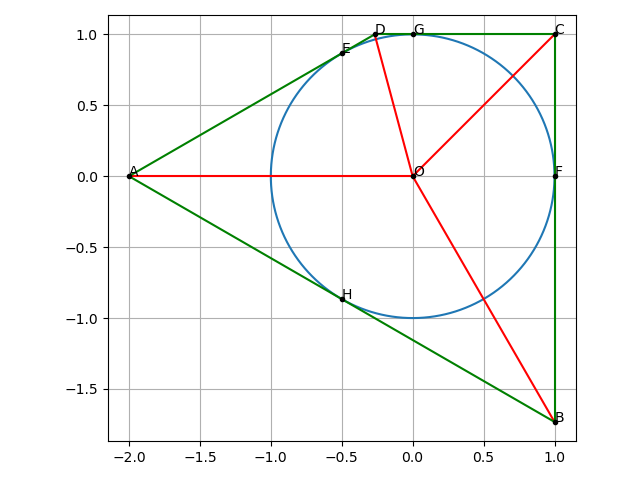
\includegraphics[width=\columnwidth]{chapters/10/10/2/13/figs/quad_circ.png}
        \caption{Angles subtended by the opposite sides of a circumscribing quadrilateral at the center of its incircle are supplementary.}
        \label{fig:chapters/10/10/2/13/quad-circ}
    \end{figure}

\item Find the equation of a circle whose centre is (3,1) and which cuts off a chord of length  6 units on the  line 2x-5y+18=0
\item Find the equation of a circle of redius 5 which is touching another circle $x^2+y^2-2x-4y-20=0$ at (5,5).
Fill in the Blanks
\begin{enumerate}[label=\thesection.\arabic*,ref=\thesection.\theenumi,resume*]
\item The equation of the circle having centre at (3,-4) and touching the line $5x+12y-12=0$ is \makebox[1cm]{\hrulefill}                     
\item The equation of the circle circumscribing the triangle whose sides are the lines $y=x+2, 3y=4x, 2y=3x$ is  \makebox[1cm]{\hrulefill}         

\end{enumerate}
